%		For public use only, fair use laws still apply
%		A tutorial template created by Chad Gibbons




%	I recommend for generic help the following website
%	http://www.emerson.emory.edu/services/latex/latex_toc.html
%	There are many good websites and forums for LaTeX
%
%	If you have a problem, google it. (ex. "How do I start my page numbers at a different number")



%%%%%%%%%%%%%%%%%%%%%%%%%%%%%%%%%%%%%%%%%%%%%%%%%%%%%%
%					 													  %
%					 													  %
%					  ALWAYS BEGIN THE PROGRAM WITH								  %
%					 													  %
%						\documentclass{class_type}								  %
%																		  %
%		Different class types have different commands associated with them, similar to header files			  %
%					 													  %
%					 													  %`
%%%%%%%%%%%%%%%%%%%%%%%%%%%%%%%%%%%%%%%%%%%%%%%%%%%%%%

\documentclass[12pt]{article}

%%%%%%%%%%%%%%%%%%%%%%%%%%%%%%%%%%%%%%%%%%%%%%%%%%%%%%
%					 													  %
%					 													  %
%				It is recommended to only use packages as you need them 						  %
%					 													  %
%	Different types of reports will consistently use specific packages; keep these in their respective templates		  %
%					 													  %
%					 													  %
%%%%%%%%%%%%%%%%%%%%%%%%%%%%%%%%%%%%%%%%%%%%%%%%%%%%%%


%\usepackage[a4paper,total={8.27in,11.69in},left=0.56in,right=0.56in,top=0.75in,bottom=1.69in]{geometry}		% 	Margins IEEE Articles
\usepackage[letterpaper,total={8.5in,11in},left=1.25in,top=1in,bottom=1in,right=1in]{geometry}		% 	Margins PDD
%\usepackage[a4paper,total={6.5in,9.375in}]{geometry}		% 	Margins MLA
%\usepackage{babel}				%	Expands text mode
\usepackage[english]{babel}
\usepackage{csquotes}				%	Permits \enquote{quote}
\usepackage{graphicx}				%	Permits \includegraphics[]{image}
\usepackage{caption}				%	Permits the void caption \caption*{}
\usepackage{titlesec}				%	Modify section titles
\usepackage{wrapfig}				% 	Insert wrappable objects like figures or tables
%\usepackage{a4wide}				% 	Expand width of body lazily
\usepackage{multicol}				% 	Permits multicolumn
\usepackage{multirow}				%	Permites utilization of multiple rows of a table
\usepackage{tocloft}				%	Permits modification of Table of Contents
\usepackage{amssymb}				%	Greek Alphabet Symbols
\usepackage{appendix}

\usepackage{scrextend}				% 	Permits padding margins of document


\graphicspath{ {./images/} }			%	Sets filepath to images folder in location of TeX Document

\usepackage[utf8]{inputenc}			%	biblatex depends on on this package
\usepackage{comment}
%\usepackage[backend=bibtex,style=numeric]{biblatex}	%	LaTeX blibliography	%% Note: ieee stle lower-cases titles past first letter (Which seems wrong)
\usepackage[backend=bibtex,style=numeric,sorting=none]{biblatex}
%\bibliographystyle{ieeetr}			% INVESTIGATE FURTHER FOR AUTO ORDERING OF BIB REFERENCES
\bibliography{FDR_Draft}				%	REMEMBER TO RENAME THIS FILE IF MOVING TO NEW .bib


%\addbibresource{hec2.bib}


			%	Makes Table of Contents Functionally a table of Hyperlinks
\usepackage{hyperref}
\hypersetup{
	colorlinks,
	citecolor= black,
	filecolor = black,
	linkcolor = blue,
	urlcolor = blue
	}

			%	Next Three Lines permit use of .tif images in \includegraphics
\usepackage{epstopdf}
\epstopdfDeclareGraphicsRule{.tif}{png}{.png}{convert #1 \OutputFile}
\AppendGraphicsExtensions{.tif}

\renewcommand{\thesection}{\Roman{section}} 
\renewcommand{\thesubsection}{\thesection.\Alph{subsection}}
\renewcommand{\thesubsubsection}{\thesection.\arabic{subsubsection}}
\setlength\cftsecnumwidth{3em}
\setlength\cftsubsecnumwidth{3em}
\setlength\cftsubsubsecnumwidth{3em}

			%	Define Abstract to be IEEE compliant (10pt, centered, roman numerals, capitalized)
\titleformat{\abstract}{\normalfont\btshape}{\Roman{section}}{1em}{\MakeUppercase}
			%	Define Sections to be IEEE compliant (10pt, centered, roman numerals, capitalized)
\titleformat{\section}{\normalfont\filcenter}{\Roman{section}.}{1em}{\MakeUppercase}
			%	Define Subections to be IEEE compliant (10pt, left, roman numerals, capitalized)
\titleformat{\subsection}{\normalfont\itshape}{\Alph{subsection}.}{1em}{}
			%	Define Subsubections to be IEEE compliant (10pt, left, roman numerals, capitalized, inline text)
\titleformat{\subsubsection}[runin]{\normalfont\itshape}{\indent\arabic{subsubsection}.)}{1em}{}
			%	Define Table of Contents to be IEEE compliant


			%	Next Two Lines Make Document San-Serif
%\renewcommand{\familydefault}{\sfdefault}		
%\usepackage{helvet}


\usepackage{textcomp}				%	For subsection symbol w/ \textsection
\usepackage{pdfpages}				%	For inserting PDF document and pages into LaTeX file
							%% 		Recommended pdfpages format : 									%%
							%%		\includepdf[pages=-,width=0.9\linewidth,pagecommand={}]{./appendices/file.pdf}		%%

\newcommand{\cross}[1][1pt]{\ooalign{ 	%	Creating footnote cross symbol
  \rule[1ex]{1ex}{#1}\cr% Horizontal bar
  \hss\rule{#1}{.7em}\hss\cr}}% Vertical bar

%\usepackage[T1]{fontspec}
\usepackage{inconsolata}				%	converts \ttfamily to consolas font
%\IfFileExists{zi4.sty}{\usepackage{zi4}}					%	renamed version of inconsolata
%{\usepackage{inconsolata}}	
%\newfontfamily{\ttconsolas}{Consolas}

  
%%%%%%%%%%%%%%%%%%%%%%%%%%%%%%%%%%%%%%%%%%%%%%%%%%%%%%%			PREAMBLE


\title{\Large \textbf{The University of Texas at Tyler\\
College of Engineering and Computer Science\\
Tyler, TX 75799\\
\hfill \\
\hfill \\[0.5em]
Final Design Report Draft \#3 \\ [0.25em] For\\[0.25em]
Wireless Charger Project}}		%note left quote command vs " = \textquotedblright
%%  FIX FONT of Sub Sub Title  >> It should fit in with the text below. <<
\author{\large \hfill \\[0.5em] \textbf{A design project to fulfill the requirements of Senior Design}\\ \textbf{ 
in the Department of Electrical Engineering}\\ \textbf{ 
at The University of Texas at Tyler
}\hfill \\ \hfill \\[0.5em]}
\date{\normalsize \flushleft  The  individuals  whose  names  and  signatures  appear  below  certify  that  the  narrative, diagrams,  figures,  tables,  calculations,  and  analyses  contained  within  this  document  are their original work except as otherwise cited.
\hfill \\ \hfill \\[0.5em]
\underline{Flory, David\space\space\space\space\space\space\space\space\space\space\space} \hspace{0.25in}
\underline{\space\space\space\space\space\space\space\space\space\space\space\space\space\space\space\space\space\space\space\space\space\space\space\space\space\space\space\space\space\space\space\space\space\space\space\space\space\space\space\space\space} \hspace{0.25in}
\underline{\today \space\space\space\space\space\space\space} \hspace{0.25in}\\
\hspace{1.8in} Signature \hspace{1.8in} Date \hfill \\ \hfill \\
\underline{Fran\c{c}a, Natasha\space\space\space\space\space\space} \hspace{0.25in}
\underline{\space\space\space\space\space\space\space\space\space\space\space\space\space\space\space\space\space\space\space\space\space\space\space\space\space\space\space\space\space\space\space\space\space\space\space\space\space\space\space\space\space} \hspace{0.25in}
\underline{\today \space\space\space\space\space\space\space} \hspace{0.25in}\\
\hspace{1.8in} Signature \hspace{1.8in} Date \hfill \\ \hfill \\
\underline{Franulovic, Franci \space\space} \hspace{0.25in}
\underline{\space\space\space\space\space\space\space\space\space\space\space\space\space\space\space\space\space\space\space\space\space\space\space\space\space\space\space\space\space\space\space\space\space\space\space\space\space\space\space\space\space} \hspace{0.25in}
\underline{\today \space\space\space\space\space\space\space} \hspace{0.25in}\\
\hspace{1.8in} Signature \hspace{1.8in} Date \hfill \\ \hfill \\
\underline{Gibbons, Chad \space\space\space\space\space\space\space} \hspace{0.25in}
\underline{\space\space\space\space\space\space\space\space\space\space\space\space\space\space\space\space\space\space\space\space\space\space\space\space\space\space\space\space\space\space\space\space\space\space\space\space\space\space\space\space\space} \hspace{0.25in}
\underline{\today \space\space\space\space\space\space\space} \hspace{0.25in}\\
\hspace{1.8in} Signature \hspace{1.8in} Date \hfill \\ \hfill \\
\underline{Sosa, Francisco \space\space\space\space\space\space\space} \hspace{0.25in}
\underline{\space\space\space\space\space\space\space\space\space\space\space\space\space\space\space\space\space\space\space\space\space\space\space\space\space\space\space\space\space\space\space\space\space\space\space\space\space\space\space\space\space} \hspace{0.25in}
\underline{\today \space\space\space\space\space\space\space} \hspace{0.25in}\\
\hspace{1.8in} Signature \hspace{1.8in} Date \hfill \\
}
%\date{12/29/2018}					%	Set permanent date or use date section as additional text real estate on the title page.
%\date{Sic et Non \\ Quid Faciendus Est}



%%%%%%%%%%%%%%%%%%%%%%%%%%%%%%%%%%%%%%%%%%%%%%%%%%%%%%%			DOCUMENT





%%%%%%%%%%%%%%%%%%%%%%%%%%%%%%%%%%%%%%%%%%%%%%%%%%%%%%
%					 													  %
%					 													  %
%					  ALWAYS BEGIN THE DOCUMENT WITH								  %
%					 													  %
%							\begin{document}									  %
%					 													  %
%					 													  %
%%%%%%%%%%%%%%%%%%%%%%%%%%%%%%%%%%%%%%%%%%%%%%%%%%%%%%


\begin{document}
\maketitle

\pagenumbering{gobble}

\pagebreak

\section*{Acknowledgments}
\pagenumbering{roman}
\indent \indent
We as a team wish to thank Indus Instruments and Dr. Sridhar Madala for being the benefactors and sponsors of our Project.  Indus Instruments develops and creates electronic devices and software to meet the needs of various industries; for instance, they provide Baylor College of Medicine critical equipment for medical research.   Dr. Sridhar Madala has been generous with our time and was critical in the initial planning phase of the project.  Dr. Madala's familiarity with FCC and international wireless transmission regulations gave clear constraints and direction to this project.  Thus, we especially thank Dr. Sridhar Madala for agreeing to be HEC-2's technical advisor.

\pagebreak

\section*{Executive Summary}
\indent \indent
The team has designed and is prototyping a managed, 30 watt wireless resonant charger for use with lithium-ion battery packs. It shall be a versatile solution to the problem of powering autonomous mobile devices fitted with moderately sized battery packs of approximately four to six 18650 cells configured for 7.4 to 14.7 volts nominal output. With an estimated cost around \$300, it fills a gap between inexpensive inductive chargers in the 5 watt range and custom 90 watt robotic power systems that have an entry level price of \$2000.\\ \indent

Our charging system is made with two essential components: a transmitter and receiver. The transmitter is supplied by standard line voltage and will be responsible for safely delivering up to 30 watts of resonant power to the receiver when in range and appropriately positioned. It shall communicate status with the receiver over a Bluetooth link and shall enable or disable power transmission when requested.\\ \indent

The receiver shall communicate with the transmitter and to a user GUI over Bluetooth links, and optionally with the user’s own application (i.e. a robot microcontroller) over a serial link. It will be capable of delivering requested power transmission and charging status information and beginning or ending the charging process. It shall cease charging on receipt of an error status from the charging circuit and will notify the user to take corrective action. Under normal conditions it will deliver power to the charging control IC, which shall charge the attached battery pack.\\ \indent

The charger may be configured to charge 7.4 to 14.7 nominal Li-Ion battery cells, which must have internal protection circuitry in accordance with UL1642 and IEC61960. Optimal configurations would include a 7.4V pack rated for 3.2A charging, a 11.1V pack rated for 2.2A charging, or a 14.8V pack rated for 1.7A charging.\\ \indent

To best demonstrate the full potential of our project, the team is pursuing optional deliverables that should be completed if time permits once the core project is completed. These stretch goals include a mobile robot capable of charging itself for continuous wireless operation and integration with a smart Li-ion battery for detailed fuel gauge and battery health status.

\pagebreak

\tableofcontents

\pagebreak

\listoffigures

\pagebreak

\listoftables

\pagebreak



	%%%%%%%%%%%%%%%%%%%%%%%%%%%%%%%%%%%%%%%%%%
	%														 %
	%														 %
	%		\hfill fills in the remaining spaces of the given line with spaces			 %
	%														 %
	%					\\ ends line           							 %
	%														 %
	%	Determine the number of "\hfill \\ " iterations in accord with the number of lines		 %
	%				   within you abstract.							 %
	%														 %
	%														 %
	%%%%%%%%%%%%%%%%%%%%%%%%%%%%%%%%%%%%%%%%%%




	%%%%%%%%%%%%%%%%%%%%%%%%%%%%%%%%%%%%%%%%%%
	%														 %
	%														 %
	%		The primary purpose of an abstract is to give sufficient information		 %
	%					on your report to inform 						 %
	%		researchers, students, grant providers, corporate executives, professors,  	 %
	%				professionals, or the audience of your intention			 %
	%		whether or not either reading or purchasing your report is necessary.		 %
	%														 %
	%														 %
	%%%%%%%%%%%%%%%%%%%%%%%%%%%%%%%%%%%%%%%%%%


\pagenumbering{arabic}

%
%	Start with defining the problem you are trying to solve and why there is still a need to solve it
%
%	+ (Problem) User devices need wireless recharging solutions
%	+ (Why need to solve exists) Shortage of cost effective mid range wireless power transfer products in market.
%
%	Is this the only product in the market? <-- we answered this >:(
%
%	
%

\section{Project Description}
\indent \indent
Our team noted a need for users to charge medium power devices via wireless charging.  After further investigation we also determined that there is a shortage of cost effective medium power wireless chargers on the market.\\ \indent

Our project is a 30 watts nominal resonant wireless charger prototype for use with 4 to 6 cell lithium ion battery packs. It is managed by a microcontroller. It may be monitored and controlled by a user GUI or directly by the target application. Unlike existing customized and proprietary robotic charging systems, our product will charge a standard battery type and be suitable for both stand-alone operations and integration into the user's own design.\\ \indent

The team has been unable to discover any equivalent products to our own for retail. The most comparable product is Wibotic's Standard High Power System\cite{WiboSHPS}, a 90 watt magnetic resonance device that is marketed to businesses designing commercial drones and robotic systems. On the lower end, nearly all unbranded, low-cost wireless chargers that are available from mass online retailers supply no more than 5W via inductive charging. For a single industrial unit, we have received a price quote for approximately \$2000 USD. Individuals and small R\&D teams that search for suitable devices through online retailers will find that these low-end transmitters are not modular and are limited to one specific purpose such as charging cell phones or key-fobs.\\ \indent

Our charging system employs magnetic resonance coupling to charge a lithium ion battery pack, delivering between 15 and 30 watts of power. The power transmitter and receiver communicates as a unified system that can provide battery management, protect against overcharging, and provide both diagnostic and telemetric information to the user and to an optional serial connection with the powered application’s control circuitry. The charging system may be monitored and controlled by the user either through an attached LCD interface or a GUI from either a Bluetooth connected PC or smartphone.\\ \indent

This wireless charging alternative's intended market consists of hobbyists and prototype designers considering a self-docking direct electrical connection solution. This is the charging method used by the Roomba\cite{RoombaEduData}, which engages with a custom dock and charges using metal contacts. While this is a cost-effective solution for a mass-produced product, wireless charging is a superior choice for autonomous mobile devices that might have a wide variety of sizes and shapes. The benefits offered by our product's wireless charging include flexible placement of the charger, a compact charging area, greater tolerance for misalignment between the charger and the target device, and the absence of exposed electrical connections.  Additionally, this product would solve the same need for OEM producers who are interested in a ``turn-key'' wireless charging solution.\\

\pagebreak
\indent
To best demonstrate the full potential of our project, the team has specified optional deliverables that include a mobile robot capable of charging itself for continuous wireless operation, fully integrated with a smart Li-ion battery for detailed fuel gauge and battery health status.\\ \indent %% (May be retracted at a later date)

The team holds that a moderate power, low cost wireless charger with accessible telemetry is useful to a small but important market of robotics hobbyists and developers, who at present, are not being served by either costly, proprietary business-to-business solutions or the low power and poorly documented inductive chargers available on the hobby market.\\ \indent

Below in Figure 1, the general flow of power from the AC to DC Wall Converter to the end user's device and information from the user is shown.
\hfill 
\begin{figure}[h!]
\centering
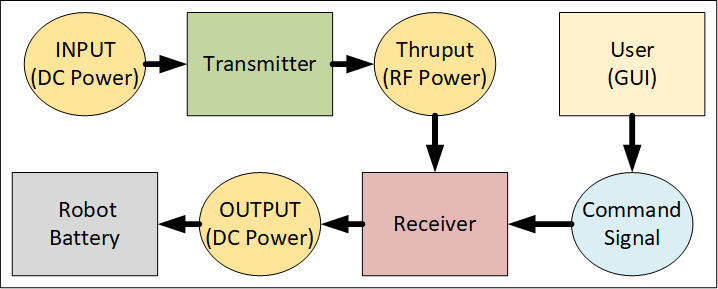
\includegraphics[width=0.84\linewidth]{black_box_power}
\caption{Operation Story Block Diagram}
\end{figure}

\indent
The project is divided between two teams: the hardware team and the software team.

\subsection{Software Team's Focus for Project}

\indent \indent
The software team is focused on two programs: the microcontrollers' firmware and the graphical user interface (GUI) software application.  The firmware operates the transmitter or receiver while the GUI allows for the user to readily monitor and interact throughout the charging process.

\hfill
\pagebreak
\hfill

\subsection{Hardware Team's Focus for Project}

\indent \indent
The hardware team is focused on producing three modular components: the receiver PCB, the transmitter PCB, and the coil module.  The image below displays how these modules operate together.

%%%%%%%%%%%%%%%

\begin{figure}[h!]
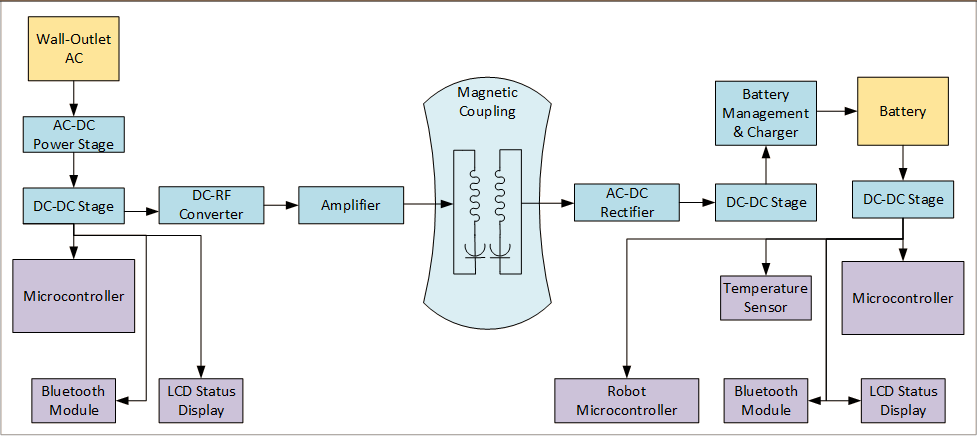
\includegraphics[width=0.92\linewidth]{power_supply_diagram}
\caption{Power Supply of Transmitter and Receiver Subsystems}
\end{figure}
\indent
While the image below explicitly separates out the receiver and transmitter modules.  Note that the completed PCB boards have a power transferring coil module affixed to them individually.
\begin{figure}[h!]
\centering
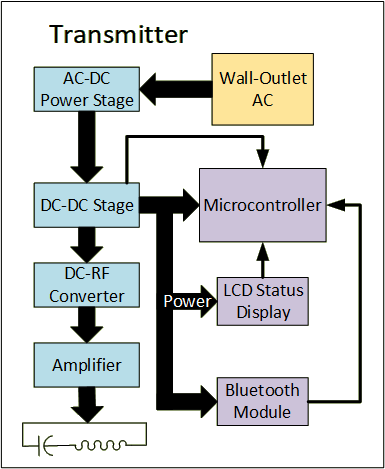
\includegraphics[width=0.41\linewidth]{transmitter_diagram.png}
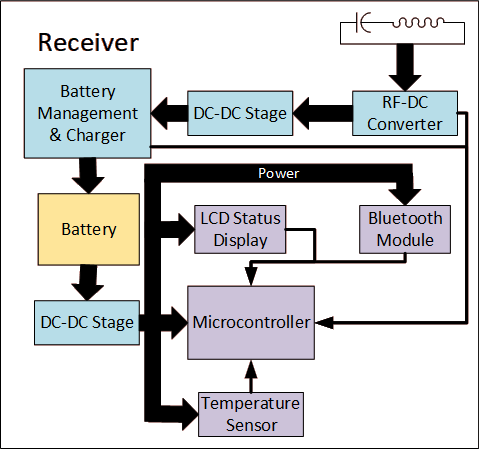
\includegraphics[width=0.532\linewidth]{receiver_diagram.png}
\caption{Transmitter and Receiver Block Diagrams}
\end{figure}
\hfill \\

%%%%%%%%%%%%%%%%%%%%%%%%5

\hfill 
\pagebreak
\hfill

\section{Final Design Specifications}

\indent
Table 1 below shows the specs of the receiver subsystem.
\hfill


	% Wrap Table Example

%\begin{wraptable}[1]{2}[3]{4}
%...
%\end{wraptable}
%Number of lines (optional)
%“r” for right and “l” for left figure placement.
%Overhang (optional)
%Width to be reserved.


%\newcolumntype{C}{>{\centering\arraybackslash} m{6cm} }  %# New column type
%\newcolumntype{R}{>{\raggedleft \arraybackslash} m{6cm} }  %# New column type

\begin{table}[h!]
\centering
\caption{Receiver Specifications}
\begin{tabular} {| r | c | }
\hline
\parbox{0.225\linewidth}{\raggedleft \hfill \\ Charge time \\  (Per 4Ah Battery Packs)\\} & ~ 5 Hours Max\\
\hline
Battery pack voltage & 14.2 V  \\
\hline
\parbox{0.25\linewidth}{\raggedleft \hfill \\  Coupling Efficiency \\ Transmitter to Receiver\\[0.4em]} & 90\%\\
\hline
\parbox{0.25\linewidth}{\raggedleft \hfill \\  AC-DC \\ Conversion Efficiency} & 80\%\\
\hline
\parbox{0.25\linewidth}{\raggedleft \hfill \\  Charging Controller \\  DC-DC converter} & 85\%\\[0.4em]
\hline
\parbox{0.25\linewidth}{\raggedleft \hfill \\  Overall Receiver \\  Conversion Efficiency} & 61.2\%\\[0.4em]
\hline
\parbox{0.25\linewidth}{\raggedleft \hfill \\  Maximum Battery \\ Charging Current} &   \parbox{0.225\linewidth}{\centering 1.25 A (14.7 V \\ battery pack)}\\
\hline
\parbox{0.25\linewidth}{\raggedleft \hfill \\  Charger Subsystem \\  Charge Protocol} &  \parbox{0.225\linewidth}{\centering \hfill \\  Constant Current \\Constant Voltage \\(Li-ION Battery)}\\
\hline
Battery Type &   \parbox{0.25\linewidth}{\centering\hfill \\  Lithium-Ion \\ (4 x18650 in Series or 2P4S Configuration)}\\
\hline
\parbox{0.25\linewidth}{\raggedleft \hfill \\  Power Negotiation} &  \parbox{0.225\linewidth}{\centering\hfill \\ Bluetooth 5 LE\\}\\
\hline
\parbox{0.25\linewidth}{\raggedleft \hfill \\  Transmitter Locator \\ Method \\[0.4em]} &   \parbox{0.225\linewidth}{\centering \hfill \\  RF Localization  [Bluetooth]}\\
\hline
Deliverable Demo &   \parbox{0.25\linewidth}{\centering \hfill \\  Self-Moving Device (Robot)}\\
\hline
Telemetry &   \parbox{0.25\linewidth}{\centering \hfill \\  Report State \\to GUI Device}\\[0.4em]
\hline
LCD display &   \parbox{0.25\linewidth}{\centering \hfill \\  Diagnostic Character \\String Display}\\
\hline
\end{tabular}
\end{table}
 
 \pagebreak
 
\indent 
Table 2 below shows the specs of the transmitter subsystem.  

\hfill
 

\begin{table}[h!]
\centering
\caption{Transmitter Specifications}
\begin{tabular} {| r | c | }
\hline
Operating frequency & 13.56 MHz\\
\hline
RF power output & 30 W\\
\hline
Max operating range & 5 cm\\
\hline
DC Power supply  & 48 V 1.25 A max.  \\
\hline
\parbox{0.275\linewidth}{\raggedleft  Conversion Efficiency\\ DC-AC\\[0.4em]}  & 80\%\\
\hline
Telemetry &\parbox{0.24\linewidth}{\centering Report State \\to GUI Device\\[0.4em]}\\
\hline
\end{tabular}
\end{table}

\indent
Table 3 below shows the communication specifications. 
\hfill

\begin{table}[h!]
\centering
\caption{Communication Link Specifications}
\begin{tabular} {| r | c | }
\hline
\parbox{0.275\linewidth}{\raggedleft Communication Medium \\[0.4em]} &  \parbox{0.24\linewidth}{\centering Bluetooth 5 LE}\\
\hline
\parbox{0.275\linewidth}{\raggedleft Protocol} &  \parbox{0.24\linewidth}{\centering \hfill\\[0.1em] L2CAP \\ (RFCOMM)\\[0.5em]}\\
% L2CAP === Logical Link Control and Adaptation Protocol (Host Stack --> One Controller with multiple devices pairing)
\hline
\end{tabular}
\end{table}

\indent
 Table 4 below shows the GUI software specifications.
 \hfill

\begin{table}[h!]
\centering
\caption{GUI Specifications}
\begin{tabular} {| r | c | }
\hline
\parbox{0.275\linewidth}{\raggedleft GUI OS} & \parbox{0.24\linewidth}{\centering \hfill \\ WinOS, IOS, \\ Linux, \& Android}\\[0.4em]
\hline
\parbox{0.275\linewidth}{\raggedleft License} &    \parbox{0.24\linewidth}{\centering LGPL 3.0} \\
\hline
\parbox{0.275\linewidth}{\raggedleft Software Architecture} &   \parbox{0.24\linewidth}{\centering \hfill \\ Model-Controller-View (MCV) Architecture\\[0.4em]} \\
\hline
\parbox{0.275\linewidth}{\raggedleft Delivery Model} &   \parbox{0.24\linewidth}{\centering \hfill \\ Open Source \\ (Free App Download)} \\[0.4em]
\hline
%\parbox{0.45\linewidth}{\raggedleft Deployment Model} &   \parbox{0.45\linewidth}{\centering Open Source / Free To Download App} \\
%\hline
\end{tabular}
\end{table}

\pagebreak

\subsection{Feasibility Study}

\indent \indent
The design consists of two subsystems: the transmitter and the receiver. This product is expected to be used by hobbyists and prototype designers for different applications that require contactless charging. There is no similar device available in the price range from \$200 to \$400.  The expected cost of the charger system is \$300. There are some commercial chargers available right now and the cost of that system is \$2000. The price of \$300 per system will make wireless charging affordable for hobbyists and freelance hardware developers.\\

\indent
The design tools such as Altium designer and Multisim simulator are available free of charge to all group members using the provided UT Tyler license. Also, parts manufacturers are providing free simulation and evaluation tools for development. In addition to the software evaluation kits may be required for testing certain parts of the system such as the microcontroller, Bluetooth module, and the battery charger controller. Most of those evaluation modules are already purchased and they are available to team members. Evaluation kits are purchased by Indus Instruments.\\

\indent
The system is designed such that it uses standard components that are available at any electronic components store and they can be purchased without restrictions. PCB fabrication will be given to a company located in China that is offering quick turnaround PCB fabrication and fast shipping. Components purchasing and printed circuit board assembly will be done at Indus Instruments. Indus Instruments have all the necessary equipment that can handle surface mount components.\\

\indent
All test equipment required for development and testing will be available. Indus Instruments will provide space and necessary test equipment for the wireless charging system prototype evaluation and testing.\\

\indent
The final product cost is estimated at around \$300 (for small quantities). Most likely for larger quantities, it is possible to decrease the cost even more. 

\pagebreak

\subsection{Microcontroller}

\indent \indent
There are four aspects to analyze: economics, technical, legal, and scheduling. A single MSP430FR5994 part costs about \$3 to \$4, while the MSP-EXP430FR5994 LaunchPad kit costs \$16.99. Considering the team only needs two of these microcontrollers (one for the transmitter and one for the receiver), this is an economic and reasonable cost. \cite{MSP430FR599x}  \cite{testKit}. On the technical side, this microcontroller’s memory, voltage supply limitations, UART and I2Cmode specifications, and overall low power consumption makes it the ideal model for our project needs \cite{MSP430FR599x}. Some of the most important standards TI’s MSP430FR5994 complies with include ANSI, JEDEC, and ESDA \cite{MSP430FR599x}. Lastly, the team already has in hands the LaunchPad kit for the microcontroller. The individual microcontrollers are also ready-to-purchase items with delivery times of less than 7 days. More testing will be done once the team has the first PCB design in hands.


\subsection{Transmitter Coil}

%%%%%%  COME BACK TO ME %%%%%%%%%%%%%%%%%%%%%%%%%%%%%%%%%%%%%%%%%%%%%%%%%%%%%%%%%%%%%%%%%%%%%%%%%%%%%%%%%%%%%%%%%%%%%%%%%%%%%%%%%%%%%%%%%%%%%%%%%%%%%%%%%%%%%%%%%%%%%%%%%%%%%%%%%%%%%%%%%%%%%%%%%%%%%%%%%%%%%%%%%%%%%%%%%%%%%%%%%%%%%%%%%%%%%%%%%%%%%%%%%%%%%%%%%%%%%%%%%%%%%%%%%%%%%%%%%%%%%%%%%%%%%%%%%%%%%%%%%%%%%%%%%%%%%%%%%%%%%%%%%%%%%%%%%%%%%%%%%%%%%%%%%%%%%%%%%%%%%%%%%%%%%%%%%%%%%%%%%%%%%%%%%%%%%%%%%%%%%%%%%%%%%%%%%%%%%%%%%%%%%%%%%%%%%%%%%%%%%%%%%%%%%%%%%%%%%%%%%%%%%%%%%%%%%%%%%%%%%%%%%%%%%%%%%%%%%%%%%%%%%%%%%%%%%%%%%%%%%%%%%%%%%%%%%%%%%%%%%%%%%%%%%%%%%%%%%%%%%%%%%%%%%%%%%%%%%%%%%%%%%%%%%%%%%%%%%%%%%%%%%%%%%%%%%%%%%%%%%%%%%%%%%%%%%%%%%%%%%%%%%%%%%%%%%%%%%%%%%%%%%%%%%%%%%%%%%%%%%%%%%%%%%%%%%%%

\indent \indent
The circular planar coil was the most inexpensive approach, the copper tubing to make the coils has an approximate value of  \$15.99. The design properties also significantly contributed to reducing the complexity of acquiring the main coil parameters. It was important to take this factor into account because of the time constraint of two months. In order to reduce the complexity in our project, the spiral planar design was the best option.\\

\indent
The calculation of the inductance formula in the planar spiral design was easier to acquire than the other two proposed solutions. This was crucial because it significantly gave the project a higher chance of matching the predestined inductance of the circuit requirement of .909 $\mu$H.\\

\indent
The economical and ethical considerations did not affect our decision making as much, due to the fact that there were not many differences. Furthermore, this design was appropriate for our project and the team does have the budget, resources and time to successfully to implement this design. \\

\indent
The planar spiral coil design allows the project to more reduces the complexity of the formulas implemented in the calculations. 

%%%%%%%%%%%%%%%%%%%%%%%%%%%%%%%%%%%%%%%%%%%%%%%%%%%%%%%%%%%%%%%%%%%%%%%%%%%%%%%%%%%%%%%%%%%%%%%%%%%%%%%%%%%%%%%%%%%%%%%%%%%%%%%%%%%%%%%%%%%%%%%%%%%%%%%%%%%%%%%%%%%%%%%%%%%%%%%%%%%%%%%%%%%%%%%%%%%%%%%%%%%%%%%%%%%%%%%%%%%%%%%%%%%%%%%%%%%%%%%%%%%%%%%%%%%%%%%%%%%%%%%%%%%%%%%%%%%%%%%%%%%%%%%%%%%%%%%%%%%%%%%%%%%%%%%%%%%%%%%%%%%%%%%%%%%%%%%%%%%%%%%%%%%%%%%%%%%%%%%%%%%%%%%%%%%%%%%%%%%%%%%%%%%%%%%%%%%%%%%%%%%%%%%%%%%%%%%%%%%%%%%%%%%%%%%%%%%%%%%%%%%%%%%%%%%%%%%%%%%%%%%%%%%%%%%%%%%%%%%%%%%%%%%%%%%%%%%%%%%%%%%%%%%%%%%%%%%%%%%%%%%%%%%%%%%%%%%%%%%%

\subsection{Transmitter}

\indent \indent
The transmitter class-E amplifier circuit was simulated at an efficiency of 98\%. The actual transmitter efficiency would be around 90\%. In the simulation, it was determined that the current required to power the class-E amplifier is 0.9 A at 30 V. The power for the transmitter will be supplied by using an external 48 V AC to DC converter followed by a step-down converter in the transmitter subsystem.\\

\pagebreak

\indent
The main concern in this subsystem is the immunity of the supporting circuits to the RF electromagnetic field generated by the transmitter coil. The transmitter coil placement must be done such that the electromagnetic field has minimal effects on the electronic circuits in the transmitter. The transmitter sensitive electronic parts may require EMI shields.\\

\indent
During the simulation, the high voltage across the coil was observed. The highest voltage observed was 320 Vpp. That voltage poses a serious electric shock hazard. Therefore, the transmitter coil insulation must be capable of withstanding voltages that are in the 500V to 1kV range to provide a safety margin for the design. One way of achieving this is to make a plastic box that would contain the transmitter coil and have insulation that is capable of withstanding voltages in the 500 V to 1000 V range.  \\

\indent
Heat dissipation in the Class E amplifier circuit is expected to be around 3W (based on the efficiency of 90\%). That dissipation will occur in inductors, capacitors (due to ESR), and the amplifier transistor. The transistor will have a proper heatsink to prevent overheating. Since the dissipation in the transistor is very small (on-resistance is 50 mΩ) the proper thermal management will be achieved on the printed circuit board. Coils used in the transmitter will be designed such that the col resistance is minimized which also will decrease the heat dissipation in the transmitter circuit.

\subsection{Receiver}

\indent \indent
There is a possibility that the receiver RF to DC stage performs with higher losses than the losses that were determined in the simulation. According to the simulation data, the RF to DC conversion will be 81\% efficient. In the system specification, the conversion efficiency is set to 80\%. It is important to keep efficiency above 80\% to prevent excessive heat generation. If received power is 25W and efficiency is  80\% then power dissipation is 5 W.   \\

\indent
The excessive heat may have adverse effects on battery life and the speed of charging \cite{TPSM265R1}. A higher temperature environment requires lower charging currents to prevent further temperature rise and damage to the battery cells. Also, excessive heat generation must be minimized to avoid the use of fans and large heat-sinks. Heat-sinks and fans would increase the cost and the size of our product.   If during the prototype test phase efficiency drops below 80\% the circuit must be redesigned to achieve the target specification efficiency. \\

\pagebreak

\indent
One problem that is likely to occur is the interference in the battery charging and communication link circuits caused by a strong electromagnetic field generated by the transmitter coil. Even though all good practices will be followed for the circuit board design the electromagnetic interference still may not be prevented. Charging circuit disruption can cause battery failure due to overcharging or overheating. If this problem occurs the additional EMI shielding will be required. The shielding includes placing metal boxes over sensitive electronic subcircuits and placing additional filters in series with DC power supplies for sensitive parts such as a microcontroller, Bluetooth module, and charger controller.

\subsection{Thermal Considerations for 3.3V and 5V Voltage Regulators}

\indent \indent
According to the simulation data both parts have small power dissipation. The largest power dissipation is 0.18 W (5.0V regulator).\\

\indent
The graph below provides thermal resistance junction to ambient as a function of the printed circuit board. The equation below can be used to find the required thermal resistance junction to ambient ($\Theta_{JA}$). The estimated ambient temperature in the transmitter is 45$^{\circ}$C.

\begin{equation}
\Theta_{JA} = \frac{125^\circ C - T_{A(max)}}{P_{D(max)}} \Bigg[\frac{^\circ C}{W}\Bigg]
\end{equation}

\noindent
$\Theta_{JA}$ = $\frac{125-45}{0.18}$ = 444.44 \Big[$\frac{^\circ C}{W}$\Big]

\noindent
The estimated transmitter PCB area will be around 100cm2. Given the board size and thermal resistance vs. board size, those regulators will have a proper heatsink.

\begin{figure}[h!]
\centering
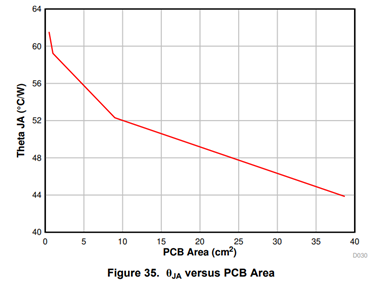
\includegraphics[width=0.82\linewidth]{pcb_JA_theta}
\caption{Thermal Resistance vs. PCB Area \cite{TPSM265R1}}
\end{figure}

\pagebreak

\noindent
Thermal considerations(for class E amplifier voltage regulator (30V, 1.0A buck converter) 

\begin{equation}
T_{A(max)} = T_{J(max)} - R_{TH} \cdot P_{TOT}
\end{equation}
\noindent
$\cdot $ P$_{TOT}$ is the total device power dissipation in [W]
\\
\noindent
$\cdot $ T$_A$ is the ambient temperature in [$^\circ$C]
\\
\noindent
$\cdot $ T$_J$ is the junction temperature in [$^\circ$C]
\\
\noindent
$\cdot $ R$_{TH}$ is the thermal resistance of the package \Big[$\frac{^\circ C}{W}$\Big]
\\
\noindent
$\cdot $ T$_{A(max)}$ is the maximum ambient temperature in [$^\circ$C]
\\
\noindent
$\cdot $ T$_{J(max)}$ is the maximum junction temperature in [$^\circ$C]
\\

\noindent
The expected ambient temperature is 40$^\circ$C (that is temperature inside the transmitter enclosure).\\
Thermal resistance for a standard board ($\Theta_{JA}$) is 62.5\Big[$\frac{^\circ C}{W}$\Big] \cite{TPS54160}.\\
From the simulation the total power dissipation is 1 W.\\
From the recommended operating conditions the maximum junction temperature is 150$^\circ$C \cite{TPS54160}.\\
Based on the data from the simulation and the datasheet the maximum ambient temperature can be determined\\
T$_{A(MAX)}$ = T$_{J(MAX)}$ - R$_{TH}$*P$_{TOT}$ \\
T$_{A(MAX)}$ = 150 – 62.5*1 = 87.5$^\circ$C

\hfill
\pagebreak
\hfill

\indent
The expected ambient temperature is lower than the maximum temperature calculated based on simulation data. Therefore, this part will operate within specified recommended conditions in the datasheet.

\subsection{Charging Subsystem}

\indent \indent
The LTC4162-L is designed to manage a power path between an external input power source Vin, an output power V$_{out}$, and an installed battery pack. When external input power greater than the battery voltage is available at V$_{in}$, the LTC4162 will route V$_{in}$ to V$_{out}$ and charge the connected battery. If external power is interrupted or falls below V$_{bat}$, battery power will be automatically routed to V$_{out}$. As long as the battery has charge or a power source exists at V$_{in}$, V$_{out}$ will be supplied with power, but the voltage will range from V$_{bat}$ to V$_{in}$. In order to provide consistent voltage to the target device output power should be drawn directly from the battery. Leaving V$_{out}$ unused allows the maximum power point tracking feature to operate with optimal efficiency.\\

\indent
The LTC4162 draws power directly from Vout and has its own internal LDO linear regulators. All other components of the wireless receiver PCB must be powered by an appropriate DC-DC stage at V$_{out}$ that can convert any potential input voltage (i.e. 7.4-35 V) to the required operating voltages of 5 V and 3.3 V. In the event that the battery is severely depleted and cannot power the microprocessor and Bluetooth interface, it will be necessary for the transmitter to be capable of initiating charging independently.\\

\indent
Since the LTC4162 has only an internal buck voltage regulator, the wireless power receiver subsystem must provide power to Vin that is higher than the voltage of the battery but below the maximum input voltage of 35V.\\

\indent
The LTC4162 approaches 95\% efficiency at recommended switching frequency when the input voltage is no more than approximately 5V above battery charging voltage, and surpasses 90\% in less ideal configurations. Heat losses will be in the range of three watts or less. It has a $\Theta_{JC}$ of 3.4 \Big[$\frac{^\circ C}{W}$\Big] and will be soldered to a four-layer PCB. The team does not anticipate any thermal management issues with this circuit.

\subsection{Battery Considerations}
\indent
Li-Ion batteries offer superb performance and high energy density, but require special attention to safety. Under normal circumstances the LTC4162-L will monitor battery voltage and avoid overcharging. A NTC thermistor will allow the LTC4162 to monitor local charging temperatures and limit current in accordance with JEIDA recommendations.\\

\pagebreak

\indent
For safety reasons, the team requires stricter battery specifications than originally planned. While our charger’s thermistor can limit charging current in response to ambient temperature extremes, it cannot monitor individual cells--particularly if the battery pack is intended to be modular. While it can recognize and respond to abnormal battery voltages or short conditions, it cannot automatically determine maximum safe charging current. Any battery pack used must have a maximum charge current greater than the maximum current delivery of the charger. Battery packs must also meet UL1642 and IEC61960 standards and contain internal protection circuitry to limit charge and discharge currents and protect against thermal runaway.\\

\indent
The LTC4162 can deliver a maximum of 3.2 amps and has an efficiency of up to 95\%. Assuming optimal efficiency and 26 W output from the wireless receiver, the charging voltage must be at least $\frac{25 W}{3.2 A}$ = 7.8 V in order to fully utilize the available power. Since the voltage of a typical Li-Ion cell is 3.7 V and the charging voltage is 4.2 V, the target battery pack should consist of two or more cells in series. The LTC4162 supports 1 to 8 cell series arrangements provided the input voltage is adequate. Optimal arrangements would include a 7.4V pack rated for 3.2 A charging, a 11.1 V pack rated for 2.2 A charging, or a 14.8 V pack rated for 1.7 A charging. The number of cells is set by selection pins and may be configured by a DIP switch or jumpers. It is not necessary to specify a specific number of cells for suitable battery packs, provided that they meet UL1642 and IEC61960 standards. The optimal balance of safe charging rates and performance will likely be found with packs utilizing six to eight 18650 cells or the equivalent. The power delivery estimates above are optimistic and actual power delivery from the charger may not reach these levels. As prototyping progresses, it will be possible to refine battery recommendations and expected charging times.\\

\indent
Ideally, up to 25 W will be delivered to the battery pack, making the battery the largest potential source of heat in our system. Since the battery pack is intended to be a modular, removable component with flexible specifications, it will not necessary for it to be enclosed with the wireless receiver PCB and receiving coil. It will be connected by an appropriate low-loss cable and connector, and exact placement will be determined by the user application. For this reason, the team has specified that only battery packs with internal temperature monitoring and protection circuitry should be used with this charger.\\

\indent
Our original specifications suggested that the charging subsystem would be capable of detailed monitoring of battery health and charge state. The team has learned that this type of information must be obtained at the individual cell level by a specialized controller which is usually integrated into the battery pack itself. Our charge subsystem can only recognize an approaching low-battery condition by a drop in voltage, and cannot estimate battery capacity except by calculation using charging voltage, charge times and currents, and such data would be of limited use considering battery aging and user-replaceability. It will be possible to notify the user and target device of a drop in battery voltage, but more detailed fuel gauge and battery health information will require an SMBus enabled smart battery. An I2C line on the MSP430FR5994 will be reserved for communication with an optional SMBus capable smart battery pack. If feasible, optional battery pack telemetry may be polled by firmware and reported to the user along with the data already available from the LTC4162.\\

\indent
All the parts and design resources needed to complete the charging and power subsystem are readily available. Constructing this subsystem within the projected time-frame is feasible.

\begin{table}[h!]
\centering
\caption{Final Design's Charging Subsystem  Specifications}
\begin{tabular} {| r | c | }
\hline
\parbox{0.3\linewidth}{\raggedleft DC-DC stage from wireless receiver to V$_{in}$} &   \parbox{0.65\linewidth}{\hfill \\
May not be necessary, pending further determination of wireless receiver output voltage}\\
\hline
\parbox{0.3\linewidth}{\raggedleft DC-DC stage from V$_{out}$} &   \parbox{0.65\linewidth}{\hfill \\
5V at 100mA; 3.3V at 100 mA}\\
\hline
\parbox{0.3\linewidth}{\raggedleft Battery Requirements} &   \parbox{0.65\linewidth}{\hfill \\
UL1642 and IEC61960 compliant Li-Ion packs with 7.4-15 V$_{DC}$ nominal output voltage}\\
\hline
\parbox{0.3\linewidth}{\raggedleft \vspace{0.4em} Maximum Charging Current} &   \parbox{0.65\linewidth}{\hfill \\
3.2A (7.4V); 2.2A (11.1V); 1.7A (14.8V)}\\
\hline
\parbox{0.3\linewidth}{\raggedleft \vspace{0.4em} Provision for optional smart battery health and fuel gauge monitoring} &   \parbox{0.65\linewidth}{\hfill \\
Reserved I2C line from MSP430FR5994 with buffering}\\
\hline
\end{tabular}
\end{table}
\hfill \\

\subsection{Microcontroller Considerations}

\indent \indent
The MSP430FR5994 has a body size that ranges from 6mm by 6mm to 12mm by 12mm depending on the package the group purchases, 8KB RAM, 68 GPIO pins, 4 I$^2$C, 4 UART, up to four serial communication ports, and 20 ADC channels. The MSP430 series include limitations that range from safety to performance \cite{MSP430FR599x}.\\

\noindent
Relevant limitations to the project include:\\

\noindent
1. ESD (Electrostatic discharge) ratings. For a human-body model, safe discharge ratings are around 500 V to 1000 V, while for a charged-device model, safe discharge ratings are around 250 V. These regulations are taken from JEDEC JS-001 and JESD22-C101 respectively \cite{MSP430FR599x}.\\

\noindent
2. Absolute maximum ratings: voltage applied to any pin must be within -0.3 V to 4.1 V, voltage difference between DVCC and AVCC pins must stay within -0.3 V to 0.3 V (if not, writing errors could occur to RAM and FRAM), and current at any device pin must have a maximum of  -2 to 2 mA \cite{MSP430FR599x}.\\

\noindent
3. Supply voltage applied should be within 1.8 V to 3.6 V, maximum ACLK frequency should be 50 kHz, and maximum SMCLK frequency should be 16 MHz \cite{MSP430FR599x}.\\

\noindent
4. For the eUSCI I$^2$C, eUSCI (enhanced universal serial communication interface) input clock frequency should not exceed 16 MHz, SCL clock frequency should not exceed 400 kHz \cite{MSP430FR599x}.


\subsection{Firmware Requirements: Transmitter}

\indent \indent
The Wireless Power Transmission Stage (Transmitter) will be controlled by an MSP430FR5994 running custom firmware. The firmware must meet the following requirements:\\

\noindent
1.) Activate or deactivate wireless transmitter.\\

\noindent
2.) Respond to commands received from a Bluetooth link with the Wireless Power Receiver Stage (Receiver), which may include requests for power delivery measurements or instructions to initiate or cease charging.\\

\noindent
3.) Continuously monitor wireless power transmitter current and voltage and calculate delivered power.\\

\noindent
4.) Automatically cease power transmission when the Receiver requests a shutdown or if severe interference is detected.\\

\noindent
5.) Communicate operating status to the Receiver via Bluetooth, and directly to the user via fault LED’s or an installed LCD.


\subsection{Firmware Requirements: Receiver}

\indent \indent
The Wireless Power Receiver Stage (Receiver) will be controlled by an MSP430FR5994 running custom firmware. The firmware must meet the following requirements:\\

\noindent
1.) Link to the Transmitter over Bluetooth.\\

\noindent
2.) Link to user GUI device over Bluetooth.\\

\noindent
3.) Link to an optional UART connection with the target device.\\

\noindent
4.) Respond to queries or instructions from the Bluetooth connection to the user GUI or from the optional UART connection.\\

\noindent
5.) Monitor charging state and battery status though I2C connection with LTC4162 and optional SMBus link with smart battery.\\

\noindent
6.) Recognize low voltage state or optional low capacity battery warning and notify the user and target device.\\

\noindent
7.) Signal the Transmitter via Bluetooth to initiate charging when instructed by the user or target device.\\

\noindent
8.) Continuously monitor wireless power receiver current and voltage and calculate delivered power.\\

\noindent
9.) Monitor reported power transmission from the Transmitter, compare it with received power, and recognize excessive power losses that could indicate unsafe interference conditions\\

\noindent
10.) In the event of excessive transmission losses, instruct the Transmitter to cease power transmission. Notify the user and target device of the error condition.\\

\indent
The Transmitter and Receiver firmware will be developed with Texas Instruments Code Composer Studio. The team has suitable Launchpad development boards and access to all necessary documentation and libraries are available. The team is composed of multiple experienced programmers in our group. The firmware requirements are limited and well-defined and completing it within our scheduled time-frame is feasible.


\subsection{Software Requirements: GUI}

The GUI will be operated on multiple platforms and rely upon QT5 to operate.  The software must fulfill the following requirements:\\

\noindent
1.) Provide connection to transmitter and receiver for the product's user that grants sufficient control over the product's hardware\\

\noindent
2.) Serve as a platform for custom messages to and from the user's device connected to the receiver.\\

\noindent
3.) Provide alert system via push notifications and continuous monitoring of the transmitter and receiver.\\

\pagebreak

\subsection{Coil Considerations}

\begin{table}[h!]
\centering
\caption{Final Design's Coil Tubing Specifications}
\begin{tabular} {| r | c | }
\hline
\parbox{0.3\linewidth}{\raggedleft
Material
} &   \parbox{0.45\linewidth}{\hfill \\
122 Copper
}\\
\hline
\parbox{0.3\linewidth}{\raggedleft
Tube Size
} &   \parbox{0.45\linewidth}{\hfill \\
1/8 [in]
}\\
\hline
\parbox{0.3\linewidth}{\raggedleft
Outter Diameter (OD)
} &   \parbox{0.45\linewidth}{\hfill \\
1/4 [in]
}\\
\hline
\parbox{0.3\linewidth}{\raggedleft
Wall Thickness
} &   \parbox{0.45\linewidth}{\hfill \\
0.049 [in]
}\\
\hline
\parbox{0.3\linewidth}{\raggedleft
Inner Diameter (ID)
} &   \parbox{0.45\linewidth}{\hfill \\
0.152 [in]
}\\
\hline
\parbox{0.3\linewidth}{\raggedleft
Fabrication
} &   \parbox{0.45\linewidth}{\hfill \\
Seamless
}\\
\hline
\parbox{0.3\linewidth}{\raggedleft
Bending Method
} &   \parbox{0.45\linewidth}{\hfill \\
By hand
}\\
\hline
\parbox{0.3\linewidth}{\raggedleft
Temper Rating
} &   \parbox{0.45\linewidth}{\hfill \\
Soft
}\\
\hline
\parbox{0.3\linewidth}{\raggedleft
Compatible Tube Fittings
} &   \parbox{0.45\linewidth}{\hfill \\
Compression, Solder Connect
}\\
\hline
\parbox{0.3\linewidth}{\raggedleft
Specifications met
} &   \parbox{0.45\linewidth}{\hfill \\
ASTM B75\\
RoHS 3(2015/863/EU) Compliant
}\\
\hline
\parbox{0.3\linewidth}{\raggedleft
Resistivity 
} &   \parbox{0.45\linewidth}{\hfill \\
1.68 x 10$^{-8}$ [$\Omega$/m]
}\\
\hline
\parbox{0.3\linewidth}{\raggedleft
Conductivity 
} &   \parbox{0.45\linewidth}{\hfill \\
5.96 x 10$^7$ [S/m]
}\\
%\hline
%\parbox{0.3\linewidth}{\raggedleft
%
%} &   \parbox{0.45\linewidth}{\hfill \\
%
%}\\
\hline
\end{tabular}
\end{table}
\hfill \\

\indent
This tubing has good corrosion resistance and excellent heat transfer qualities. All tubing meets international standards for copper tubing. Important to note: Tube size is an accepted industry designation, not an actual size  \cite{rfCond}.

\begin{table}[h!]
\centering
\caption{Final Design's Receiver Coil Specifications}
\begin{tabular} {| r | c | }
\hline
\parbox{0.3\linewidth}{\raggedleft
Outside Diameter of Coils (Do) 
} &   \parbox{0.45\linewidth}{\hfill \\
90 mm
}\\
\hline
\parbox{0.3\linewidth}{\raggedleft
 Number of Turns 
} &   \parbox{0.45\linewidth}{\hfill \\
4
}\\
\hline
\parbox{0.3\linewidth}{\raggedleft
Length
} &   \parbox{0.45\linewidth}{\hfill \\
729.6 mm
}\\
\hline
\parbox{0.3\linewidth}{\raggedleft
Spacing
} &   \parbox{0.45\linewidth}{\hfill \\
4.81 mm
}\\
\hline
\parbox{0.3\linewidth}{\raggedleft
Width of Tubing
} &   \parbox{0.45\linewidth}{\hfill \\
3.175 mm
}\\
\hline
\parbox{0.3\linewidth}{\raggedleft
Inner Diameter (Di) 
} &   \parbox{0.45\linewidth}{\hfill \\
26.12 mm
}\\
\hline
\parbox{0.3\linewidth}{\raggedleft
Winding Radius 
} &   \parbox{0.45\linewidth}{\hfill \\
29.03 mm
}\\
\hline
\parbox{0.3\linewidth}{\raggedleft
Radial Depth 
} &   \parbox{0.45\linewidth}{\hfill \\
31.94 mm
}\\
\hline
\parbox{0.3\linewidth}{\raggedleft
Inductance
} &   \parbox{0.45\linewidth}{\hfill \\
909.66 nH.
}\\
\hline
\parbox{0.3\linewidth}{\raggedleft
Capacitance
} &   \parbox{0.45\linewidth}{\hfill \\
150.55 pF
}\\
\hline
\parbox{0.3\linewidth}{\raggedleft
Frequency
} &   \parbox{0.45\linewidth}{\hfill \\
13.6 MHz
}\\
\hline
\parbox{0.3\linewidth}{\raggedleft
Resistance (Dc) 
} &   \parbox{0.45\linewidth}{\hfill \\
1.5462 m$\Omega$
}\\
\hline
\parbox{0.3\linewidth}{\raggedleft
Total Resistance 
} &   \parbox{0.45\linewidth}{\hfill \\
69.46 m$\Omega$
}\\
\hline
\parbox{0.3\linewidth}{\raggedleft
Quality Factor 
} &   \parbox{0.45\linewidth}{\hfill \\
1119.09
}\\
\hline
%\parbox{0.3\linewidth}{\raggedleft
%
%} &   \parbox{0.45\linewidth}{\hfill \\
%
%}\\
%\hline
\end{tabular}
\end{table}
\hfill \\


\subsection{Specification Summary}

\begin{table}[h!]
\centering
\caption{Final Design's Receiver Specifications}
\begin{tabular} {| r | c | }
\hline
\parbox{0.3\linewidth}{\raggedleft
Charge time(4Ah Battery Pack)
} &   \parbox{0.65\linewidth}{\hfill \\
5 Hours Max
}\\
\hline
\parbox{0.3\linewidth}{\raggedleft
Battery pack voltage
} &   \parbox{0.65\linewidth}{\hfill \\
User Selectable: 7.4V-14.2 V
}\\
\hline
\parbox{0.3\linewidth}{\raggedleft
Coupling Efficiency Transmitter to Receiver %\vspace{0.2em}		%%% 			<---- 		THIS WORKS				%%%
} &   \parbox{0.65\linewidth}{\hfill \\
90\%
}\\
\hline
\parbox{0.3\linewidth}{\raggedleft
AC-DC Conversion Efficiency
} &   \parbox{0.65\linewidth}{\hfill \\
80\% 
}\\
\hline
\parbox{0.3\linewidth}{\raggedleft
Charging Controller DC-DC Converter
} &   \parbox{0.65\linewidth}{\hfill \\
85\%
}\\
\hline
\parbox{0.3\linewidth}{\raggedleft
Overall Receiver Conversion Efficiency
} &   \parbox{0.65\linewidth}{\hfill \\
61.2\%
}\\
\hline
\parbox{0.3\linewidth}{\raggedleft
Battery Requirements:
} &   \parbox{0.65\linewidth}{\hfill \\
UL1642 and IEC61960 compliant Li-ion packs.
}\\
\hline
\parbox{0.3\linewidth}{\raggedleft
Maximum Battery Charging Current
} &   \parbox{0.65\linewidth}{\hfill \\
3.2A (7.4V); 2.2A (11.1V); 1.7A (14.8V)
}\\
\hline
\parbox{0.3\linewidth}{\raggedleft
Charger Subsystem Charge Protocol
} &   \parbox{0.65\linewidth}{\hfill \\
Constant Current Constant Voltage (Li-Ion Battery)
}\\
\hline
\parbox{0.3\linewidth}{\raggedleft
Battery Type 
} &   \parbox{0.65\linewidth}{\hfill \\
UL1642 and IEC61960 compliant Li-Ion packs; 7.4-15 VDC nominal output voltage.
}\\
\hline
\parbox{0.3\linewidth}{\raggedleft
Power Negotiation
} &   \parbox{0.65\linewidth}{\hfill \\
Using Bluetooth 5 LE
}\\
\hline
\parbox{0.3\linewidth}{\raggedleft
Deliverables
} &   \parbox{0.65\linewidth}{\hfill \\
Wireless resonant charger with approximately 30W power transmission capability.\\
Stretch Goal: a mobile device to demonstrate autonomous charging.
}\\
\hline
\parbox{0.3\linewidth}{\raggedleft
Telemetry
} &   \parbox{0.65\linewidth}{\hfill \\
Report State to GUI Device
}\\
\hline
\parbox{0.3\linewidth}{\raggedleft
LCD display
} &   \parbox{0.65\linewidth}{\hfill \\
Diagnostic Data\\
Character String Display
}\\
\hline
%\parbox{0.3\linewidth}{\raggedleft
%
%} &   \parbox{0.65\linewidth}{\hfill \\
%
%}\\
%\hline
\end{tabular}
\end{table}
\hfill \\


\begin{table}[h!]
\centering
\caption{Final Design's Transmitter Specifications}
\begin{tabular} {| r | c | }
\hline
\parbox{0.3\linewidth}{\raggedleft
Operating Frequency
} &   \parbox{0.65\linewidth}{\hfill \\
13.56 MHz
}\\
\hline
\parbox{0.3\linewidth}{\raggedleft
RF Power Output
} &   \parbox{0.65\linewidth}{\hfill \\
30 W
}\\
\hline
\parbox{0.3\linewidth}{\raggedleft
Max. Charging Distance
} &   \parbox{0.65\linewidth}{\hfill \\
30 cm
}\\
\hline
\parbox{0.3\linewidth}{\raggedleft
DC Power supply
} &   \parbox{0.65\linewidth}{\hfill \\
48V 1.25A min.
}\\
\hline
\parbox{0.3\linewidth}{\raggedleft
Conversion Efficiency DC-AC
} &   \parbox{0.65\linewidth}{\hfill \\
80\%
}\\
\hline
\parbox{0.3\linewidth}{\raggedleft
Telemetry
} &   \parbox{0.65\linewidth}{\hfill \\
Report State to Receiver
}\\
\hline
%\parbox{0.3\linewidth}{\raggedleft
%
%} &   \parbox{0.45\linewidth}{\hfill \\
%
%}\\
%\hline
\end{tabular}
\end{table}
\hfill \\


\begin{table}[h!]
\centering
\caption{Final Design's Communication Link Specifications}
\begin{tabular} {| r | c | }
\hline
\parbox{0.3\linewidth}{\raggedleft
 Communication Medium
} &   \parbox{0.65\linewidth}{\hfill \\
Bluetooth 5 LE
}\\
\hline
\parbox{0.3\linewidth}{\raggedleft
Protocols
} &   \parbox{0.65\linewidth}{\hfill \\
GUI: Host Controller Interface (HCI)\\
Receiver-\>transmitter: Synchronous Connection-Oriented (SCO) link
}\\
\hline
%\parbox{0.3\linewidth}{\raggedleft
%
%} &   \parbox{0.45\linewidth}{\hfill \\
%
%}\\
%\hline
\end{tabular}
\end{table}
\hfill \\


\begin{table}[h!]
\centering
\caption{Final Design's GUI Specifications}
\begin{tabular} {| r | c | }
\hline
\parbox{0.3\linewidth}{\raggedleft
OS
} &   \parbox{0.65\linewidth}{\hfill \\
WinOS, IOS, Linux, \& Android
}\\
\hline
\parbox{0.3\linewidth}{\raggedleft
License
} &   \parbox{0.65\linewidth}{\hfill \\
 LGPL 3.0
}\\
\hline
\parbox{0.3\linewidth}{\raggedleft
Software Architecture
} &   \parbox{0.65\linewidth}{\hfill \\
Model-Controller-View (MCV) Architecture
}\\
\hline
\hline
\parbox{0.3\linewidth}{\raggedleft
Delivery Model 
} &   \parbox{0.65\linewidth}{\hfill \\
Open Source\\
Free App Download
}\\
\hline
%\parbox{0.3\linewidth}{\raggedleft
%
%} &   \parbox{0.45\linewidth}{\hfill \\
%
%}\\
%\hline
\end{tabular}
\end{table}
\hfill \\

\subsection{Ethical and Professional Considerations}

\subsubsection{Public Health:}
Life preserving medical equipment requires concern in the transmission of powerful RF charging signals that may interfere with the medical equipment. We will adhere to FCC standards for intentional radiators and ensure that the charger transmitter does not exceed FDA guidelines for RF emission. Our design will be informed by the guidelines of the National Council on Radiation Protection and Measurements (NCRP) and the Institute of Electrical and Electronics Engineers (IEEE).
%This device provides a means of attention to the expulsion of battery acid or other wastes from the battery chamber.  It seeks to minimize harmful by-products in the use of batteries by properly maintaining stable temperatures and observing relationships within the battery chamber itself via a thermal sensor.\\ \indent
 
\subsubsection{Safety and Welfare:}
Our design may contribute to public safety and welfare by easing the development of robotic systems intended to handle hazardous materials, work in narrow spaces, high temperature environments, or in vacuum. We will follow industry best practices for safe charging, such as current limiting and temperature monitoring, to minimize the risk of battery failure.

\pagebreak

\subsubsection{Global Factors:}
The pressures of governing bodies are to be taken into consideration in any choice this project takes; however, we are primarily concerned with the US governing bodies and then the EU bodies in order to streamline our development process to hit the largest market base possible.  Additionally, Canadian and Mexican regulations would be considered as immediate market options.\\
In an alternate vein, there are sourcing questions that must be investigated before production in order to conform with internation laws and prevent being banned from specific global markets whether at home or abroad.

\subsubsection{Societal factors}
The source code will be educational as well as providing value to the device itself.  The design's modular intention will permit versatile implementations at work or at home.  The product should serve influenceable groups such as teenagers, helping them enter STEM related fields.\\
The product as a whole should be considered in a way that would encourage further education in the classroom in physics.  Likewise, the production of the product should foster a community between the product's programmers and engineers.

\subsubsection{Environmental factors:}
This concern requires continual attention for any anomalies concerning the battery cells.  The device cannot account for all of these concerns, but should maintain labeling that makes the customer aware of such concerns that may be caused by their device.  The project must provide a means of emergency shut off by some interrupt port that is always active.  The operating robot, the user via a GUI, and the receiver itself must have this ability to turn off the charging feature of the receiver.

\subsubsection{Economic factors:}
The device could fulfill legal requirements for a client, and, in that case, a custom suite would be developed in the software at a premium to satisfy a client's needs.  Additionally, creating a lightweight, low-cost production process is critical in maximizing profits.  The open-source market also provides extensive free advertising momentum when capitalized successfully.  Additionally, the product would assist in producing other products, especially in research and development. \\

\hfill

\begin{table}[h!]
\centering
\caption{Ethical and Professional Considerations}
\begin{tabular} {| r | c | }
\hline
\parbox{0.3\linewidth}{\raggedleft Public Health} &   \parbox{0.65\linewidth}{\hfill \\
$\cdot$ Medical Equipment RF Exposure \\ $\cdot$ Electrical Shock \\ $\cdot$ Chemical Exposure}\\
\hline
\parbox{0.3\linewidth}{\raggedleft Safety and Wellness} &   \parbox{0.65\linewidth}{\hfill \\
$\cdot$ RF Bandwidth Jamming \\ $\cdot$ Electrical Shock \\ $\cdot$ Chemical Exposure}\\
\hline
\parbox{0.3\linewidth}{\raggedleft Global Factors} &   \parbox{0.65\linewidth}{\hfill \\
$\cdot$ International Governing Bodies \\ $\cdot$ Sourcing Restrictions \\ $\cdot$ Inter-Market Penetrability}\\
\hline
\parbox{0.3\linewidth}{\raggedleft Societal Factors} &   \parbox{0.65\linewidth}{\hfill \\
$\cdot$ Open-Source Capitalization\\ $\cdot$ STEM Educational Resources \\ $\cdot$ Professional Organizations \\ $\cdot$ Customer Privacy \& Security}\\
\hline
\parbox{0.3\linewidth}{\raggedleft Environmental Factors} &   \parbox{0.65\linewidth}{\hfill \\
$\cdot$ Chemical Pollution\\ $\cdot$ User Environmental Awareness\\ $\cdot$ Emergency Shut Off Cases}\\
\hline
\parbox{0.3\linewidth}{\raggedleft Economic Factors} &   \parbox{0.65\linewidth}{\hfill \\
$\cdot$ Open-Source Capitalization\\ $\cdot$ Specialty Clientele\\ $\cdot$ Rapid Agile-Deployment\\ $\cdot$ Light-Weight Production}\\
\hline
\end{tabular}
\end{table}
\hfill \\

\pagebreak


\section{Design Solution}

\subsection{Product Architecture}

\indent \indent
The wireless charger system consists of two main subsystems, the receiver and the transmitter.  The transmitter is powered by an external AC/DC 48 V power supply. The transmitter subsystem converts DC power into RF power to drive the transmitter coil. The transmitter has a microcontroller that communicates with the receiver and controls its wireless power transfer.  The receiver has a receiving coil and capacitor that completes a 13.56 MHz parallel LC resonant circuit. The magnetic field generated by the transmitter induces an electric current in the receiving coil. The received power is rectified and transferred to the battery charger circuit. Also, the receiver has a microcontroller that communicates with the transmitter and indirectly controls transmitter circuits such as the wireless power transfer circuit. The receiver also communicates with remote devices such as tablets,tw phones, or computers to provide telemetry data. \\ 

\hfill
\pagebreak


\begin{figure}[h!]
\centering
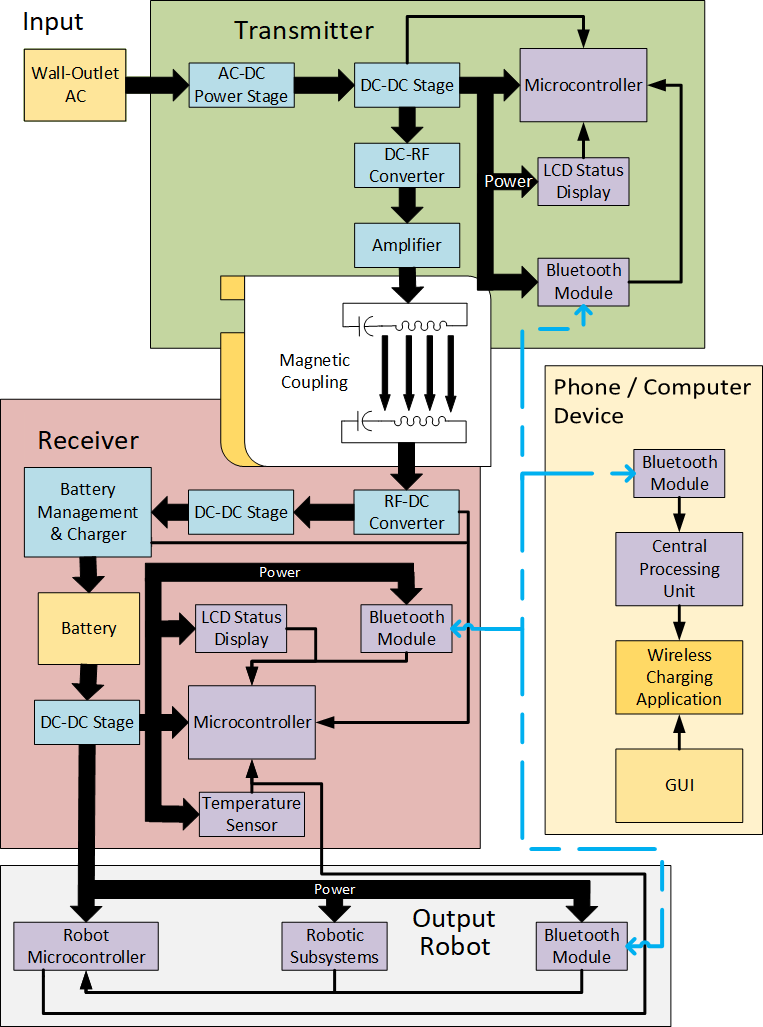
\includegraphics[width=0.88\linewidth]{total_diagram}
\caption{System Level Block Diagram}
\end{figure}

\hfill
\pagebreak

The graphical user interface (GUI) displays information with lists, data feeds, and visual aids that keep track of the battery’s charge and any information passed along by the receiver to the user’s remote device.   The GUI’s information on each device’s connection and charging information allows real-time troubleshooting of each device.\\

\indent
The GUI Wireframe image below provides an example of how the GUI is structured.  The selection widget shall be used to select between receiver devices to connect to.  The top panel is reserved for battery monitoring.  The Info panel utilizes wifi symbols to indicate connection status between devices while the lightning bolts reflect their on-going charging status.  The bottom text panel is reserved for general warnings and information.\\

\hfill

\begin{figure}[h!]
\centering
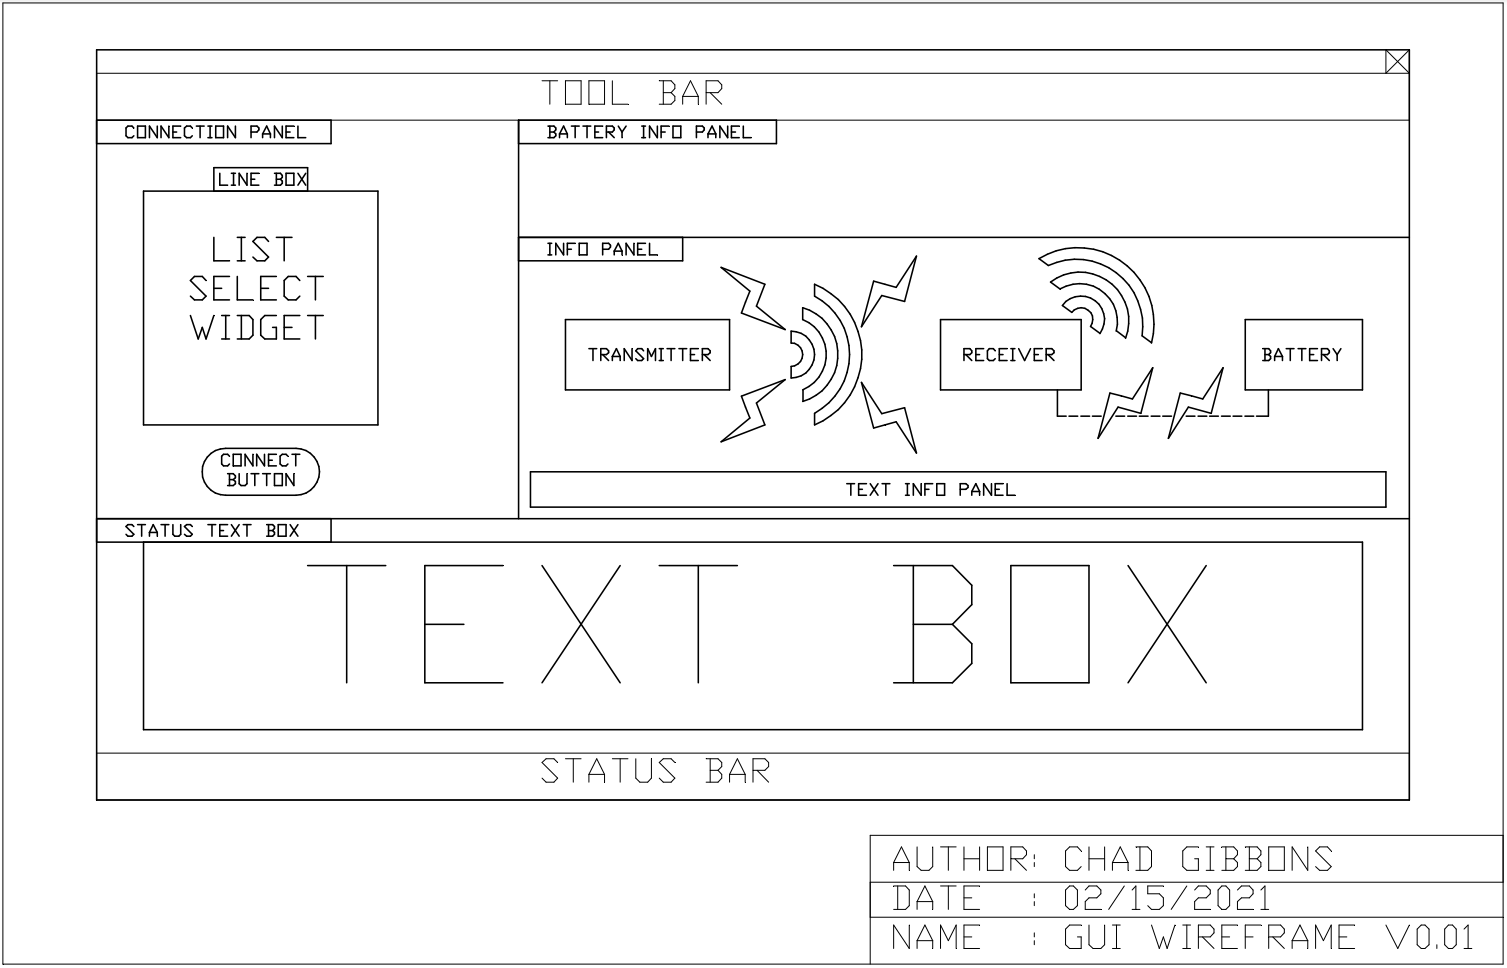
\includegraphics[width=0.88\linewidth]{gui_wireframe}
\caption{GUI Wireframe Diagram}
\end{figure}

\hfill

\pagebreak

\subsection{Hardware Subsystems}

\subsubsection{Transmitter Subsystem} The transmitter circuit requires a 48 V power supply that will be down-regulated to 30V, 5V, and 3.3V.  30V is used by a coil driver (class E amplifier).  5 V supply will be used for the LCD and class E amplifier buffer.  3.3V is used by digital circuits such as microcontroller and Bluetooth.\\

\indent
The block diagram below shows internal voltage regulator connections.

\hfill

\begin{figure}[h!]
\centering
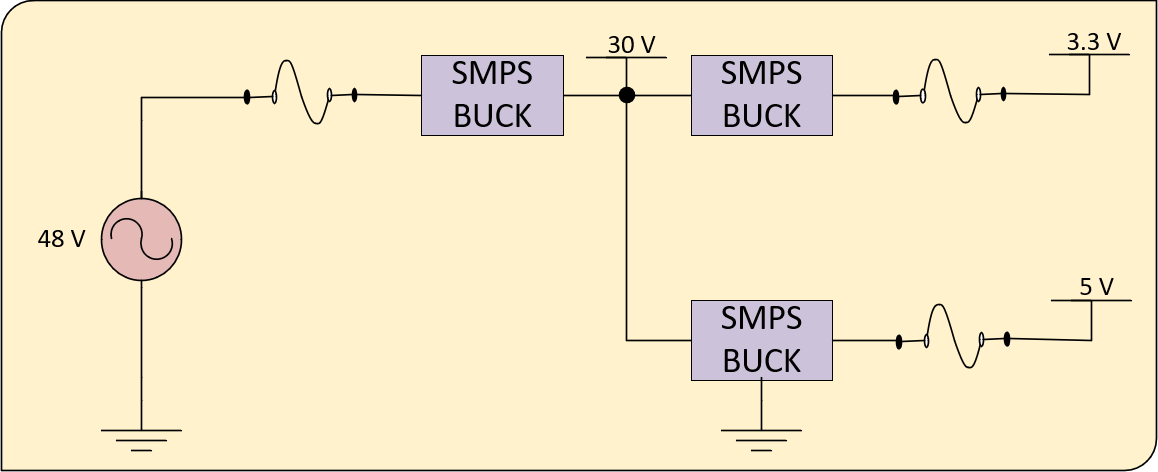
\includegraphics[width=0.88\linewidth]{trans_sub_volt_reg.png}
\caption{Transmitter Subsystem Voltage Regulator}
\end{figure}

\pagebreak

\indent
The transmitter subsystem block diagram below illustrates how transmitter subcircuits interact with each other.  The microcontroller is used to control most of the circuits in the transmitter subsystem.  The Bluetooth module is connected to the microcontroller using the UART interface with flow control (RTS and CTS lines). The Bluetooth module is connected to the circuit that controls display contrast. The display parallel I/O interface is connected to the microcontroller through a level shifter. Also, the transmitter has four multipurpose user buttons that can be used to set the different modes of operations. 

\hfill

\begin{figure}[h!]
\centering
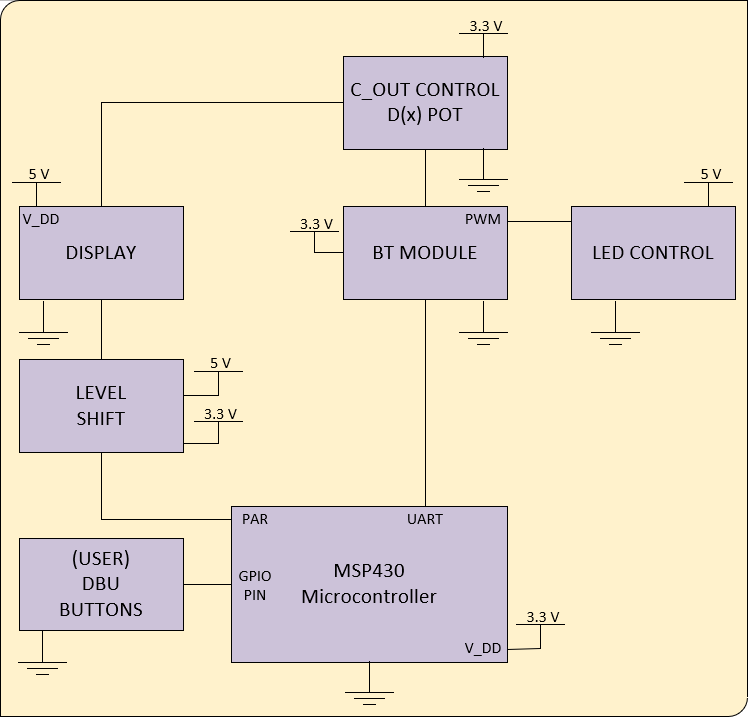
\includegraphics[width=0.88\linewidth]{controller_block}
\caption{Transmitter Subsystem Block Diagram}
\end{figure}

\hfill

\pagebreak

\indent
The block diagram below illustrates the power transmission or DC to RF converter subcircuit.  The subcircuit has an oscillator, buffer, and a coil driver.  The 13.56 MHz signal is generated by a temperature-compensated crystal oscillator. The output of the oscillator is buffered using the GaN FET driver. A tuned switching power amplifier, also known as a Class E amplifier, is used to drive the transmitter coil where a GaN FET is used as a single-pole switching element. The transmitter coil and capacitors in series create the resonant LC circuit.\\

\hfill

\begin{figure}[h!]
\centering
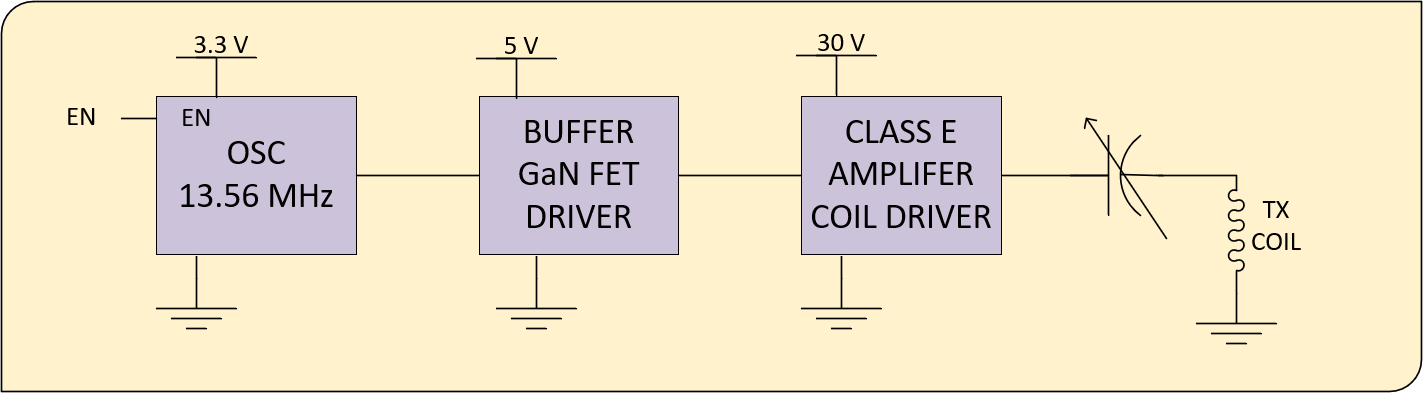
\includegraphics[width=0.88\linewidth]{trans_coil}
\caption{Coil Driver Subcircuit}
\end{figure}

\hfill

\indent
The schematic diagram for the microcontroller (U2: MSP430FR5994), Bluetooth module (MD1 RN4870) display connector P3, the display illumination control (U5: MCP6001T-I/OT, U6: NUD3112LT1G), and LCD contrast control (U7: MCP4531-103E/MS) can be found in appendix NN.\\

\indent
The input power is supplied by an external AC/DC SMPS (Switched Mode Power Supply) converter. The power output of the buck SMPS is protected by a PPTC resettable fuse as short circuit protection. The fuse rating is 2.5A. A 48V power is converted to 30V which is used by the class E amplifier’s 5V buck converter and 3.3V buck converter. Each SMPS module output has overcurrent protection using resettable PPTC fuses. Both fuses are 0.5A rated.
Both low voltage regulators (5V and 3.3V) have additional filtering at their outputs using ferrite beads and 0.1 $\mu$F capacitors.

\pagebreak

\indent
Voltage regulators are shown below

\hfill

\begin{figure}[h!]
\centering
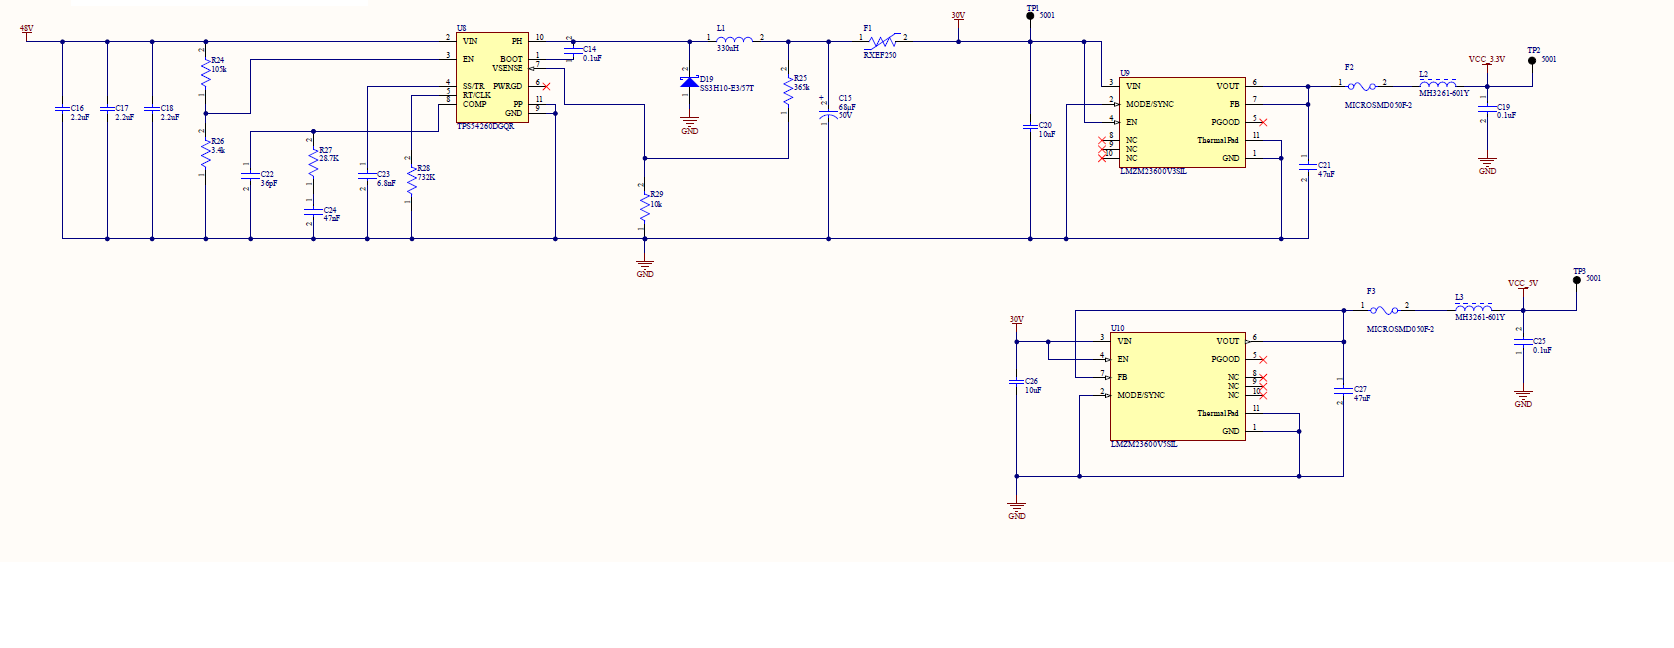
\includegraphics[width=0.925\linewidth]{tx_smps}
\caption{SMPS Subcircuit}
\end{figure}

\indent
The output of the temperature-compensated crystal oscillator (Y2) is connected to the GaN FET driver (U11: LM5112) which is connected to a GaN FET ( Q1: EPC2019). the output of the class E amplifier is connected to the transmitter coil. The amplifier circuit has a peak detector (R30, R35, D20, C36 and R36) to detect the peak voltages of its output. The voltage on the peak detector will be sampled using the microcontroller’s ADC in order to validate the receiver’s presence via loading effects on the coil.\\

\indent
The coil driver circuit is shown below 
\hfill

\begin{figure}[h!]
\centering
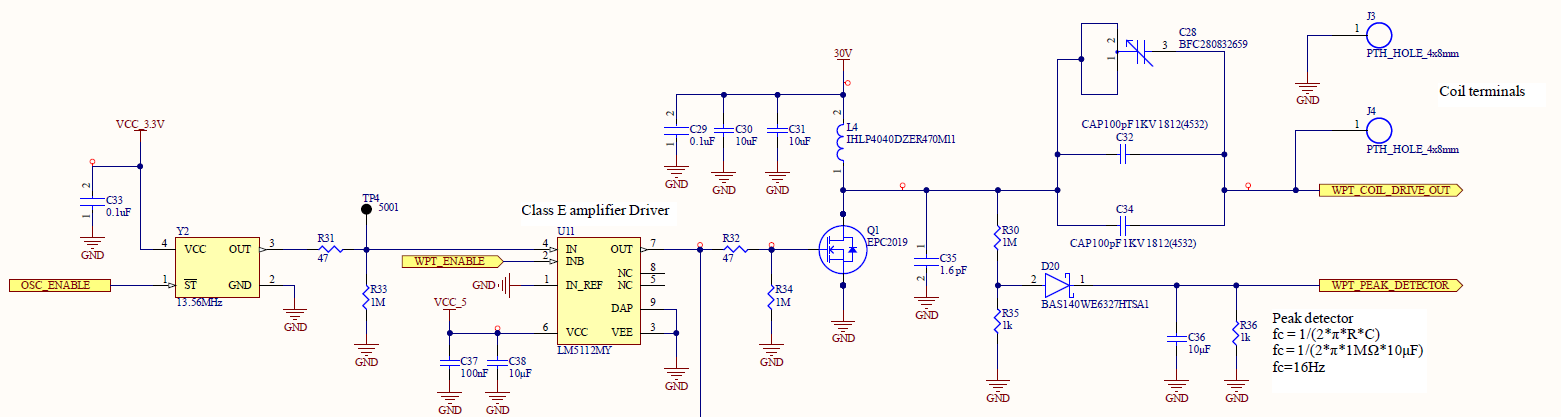
\includegraphics[width=0.925\linewidth]{tx_dc_rf_driver}
\caption{Transmitter Subcircuit}
\end{figure}

\indent
The transmitter subsystem function control and communication circuits schematic diagram shows the microcontroller (U2: MSP430FR5994), Bluetooth module (MD1 RN4870) display connector P5, the display illumination control (U5: MCP6001T-I/OT, U6: NUD3112LT1G), and LCD contrast control (U7: MCP4531-103E/MS). The schematic diagram can be found in appendix NN.

\pagebreak

\subsubsection{Receiver Subsystem} The main components in the receiver microcontroller subcircuit are identical to the transmitter microcontroller subcircuit.\\

\indent
The diagram below shows connections between receiver subcircuits. 
\hfill

\begin{figure}[h!]
\centering
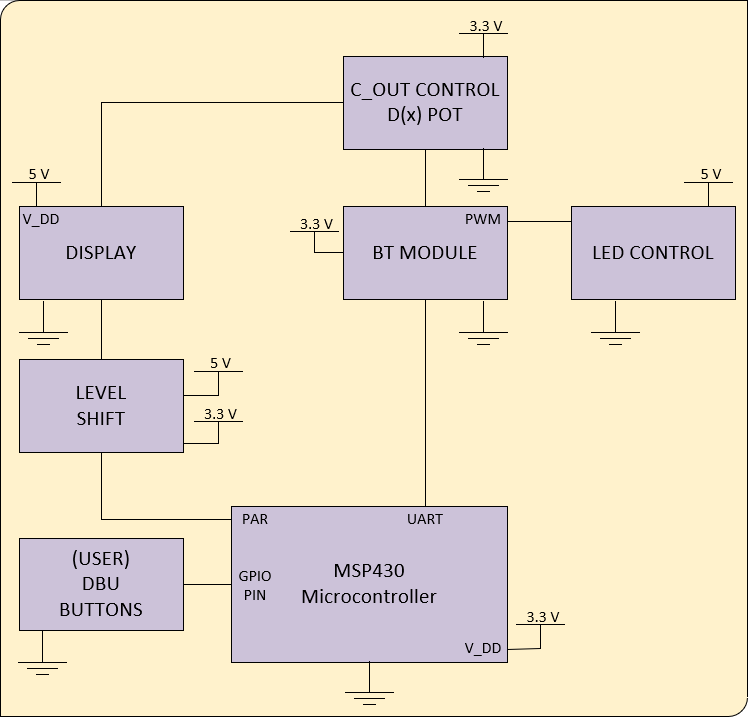
\includegraphics[width=0.88\linewidth]{controller_block.png}
\caption{Receiver Subsystem Block Diagram}
\end{figure}

\hfill

\pagebreak
\indent
The receiver coil and parallel capacitor are acting as resonant tank circuit at a frequency of 13.56 MHz. The received power is rectified using a full wave rectifier bridge and then supplies to the battery charger circuit. The rectifier output voltage and current are constantly sampled by the microcontroller to determine instantaneous received power. The battery pack is connected to the charger for charging and the battery pack SMbus interface is connected to the microcontroller. \\

\indent
The diagram below shows the receiver’s charging subcircuits.
\hfill

\begin{figure}[h!]
\centering
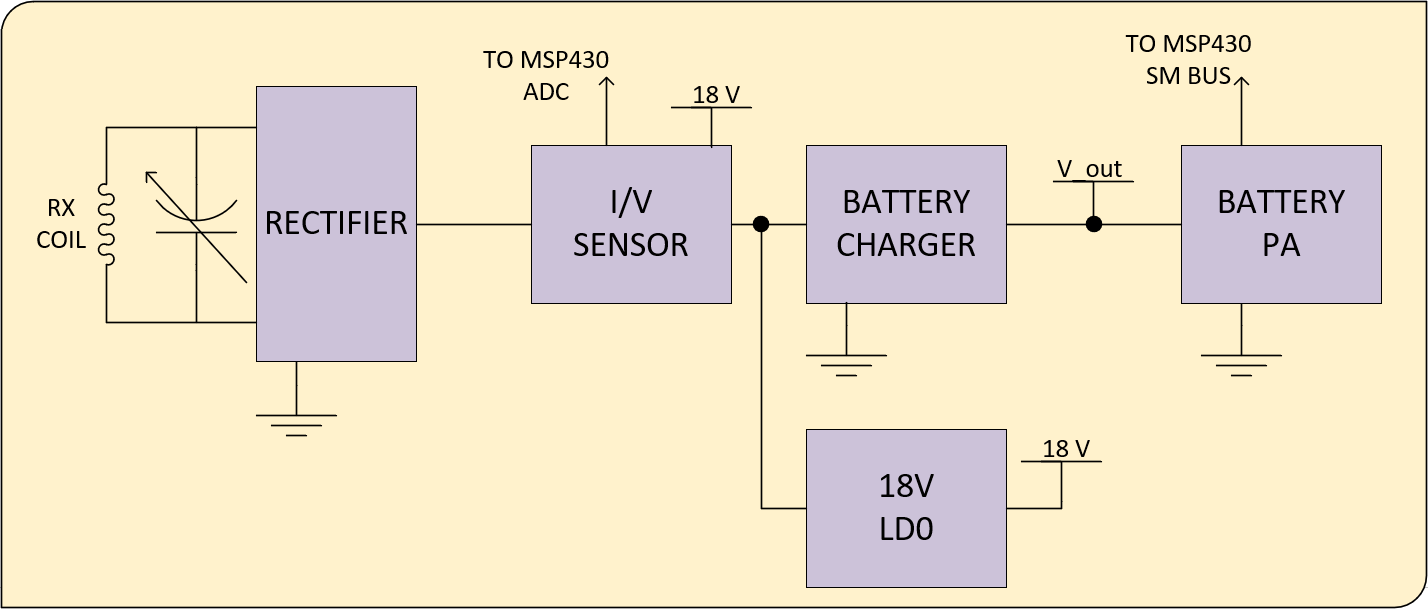
\includegraphics[width=0.88\linewidth]{recv_coil}
\caption{Receiver Coil Subsystem Block Diagram}
\end{figure}

\indent
The diagram below shows the voltage regulators utilized in powering the receiver’s digital circuits and draws power from the battery pack directly.
\hfill

\begin{figure}[h!]
\centering
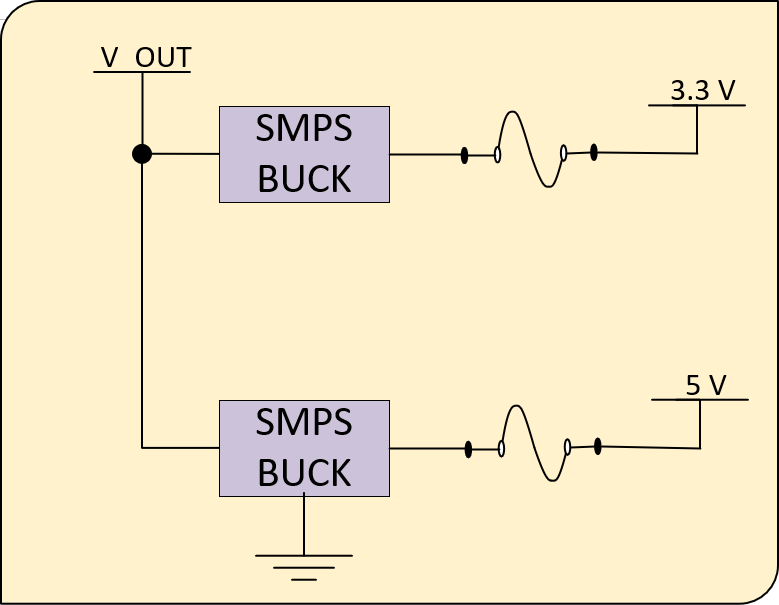
\includegraphics[width=0.45\linewidth]{recv_sub_volt_reg}
\caption{Receiver Voltage Regulator}
\end{figure}

\hfill
\pagebreak

\indent
On the receiver, battery management and power delivery functions are performed by the LTC4162-L monolithic charging controller. It handles many important battery testing and safety procedures automatically. Batteries are tested before charging, and should abnormal charging currents or voltages be detected the LTC4162-L will cease charging without firmware intervention. If conditions fall outside the preset limits a microcontroller interrupt may be triggered via the SMBALERT line for further error handling. The microcontroller firmware may read and change the LTC4162 status over an SMBus interface at any time.\\

\indent
A RRC smart battery will handle cell monitoring, balancing, and charging capacity measurement. It will automatically limit charge and discharge current to ensure safe functioning. Any one of a family of smart batteries may be connected to a keyed cable connector that ensures correct polarity and an SMBus connection. The SMBus interface will communicate with the microcontroller firmware to provide battery charge capacity and health information to the user.\\

\indent
Charger subcircuit is realized using LTC4162EUFD-SAD integrated circuit and may be found in Appendix A.2.\\

\indent
The power receiver subcircuit consists of the receiver coil, rectifier bridge, voltage sensor, and current sensor on the DC side of the circuit and feeds into the battery charging subcircuit. The rectifier bridge is designed using silicon carbide Schottky diodes.\\

\indent
DC Voltage detector and current sensor will be used to determine received power levels which can be used as an indication of transmitter-receiver inductive coupling. DC Voltage levels and current are sampled using the MSP430FR5994 AD converter.\\

\indent
The RF receiver rectifier and power sensor are shown below and can be found in larger print in Appendix A.3.%while the subcircuits can be found in their unified state in Appendix A.3.

\hfill

\begin{figure}[h!]
\centering
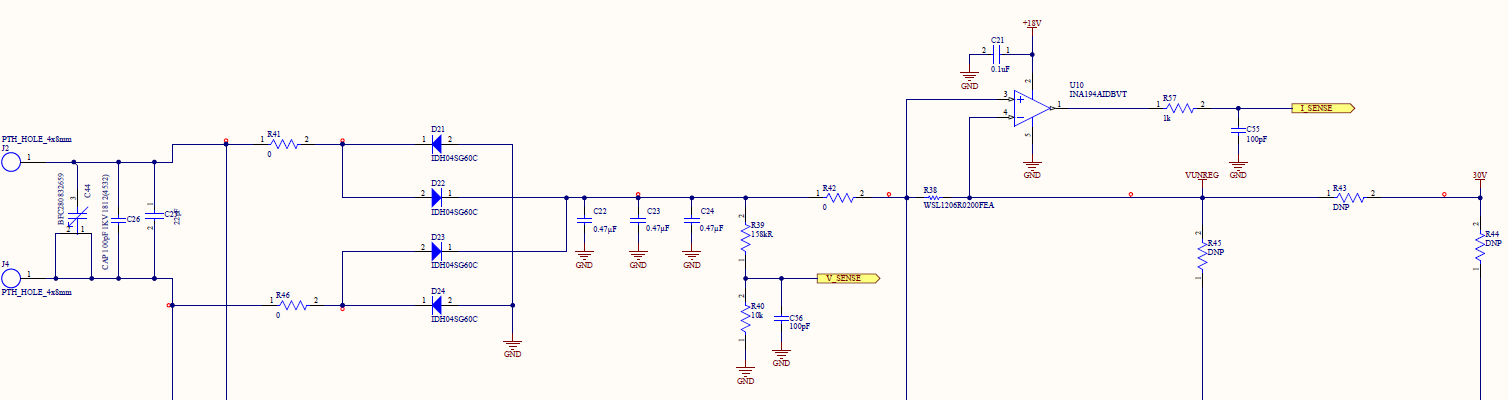
\includegraphics[width=0.88\linewidth]{rx_dc_rf_conv}
\caption{Rectifier and Power Sensor Subcircuit}
\end{figure}

\hfill

\pagebreak

\subsubsection{Planar Coil Inductor} The transmitter and receiver utilize identical planar coils in the wireless power transfer process with an inductance of 0.909 $\mu$H. The coils utilize copper tubing to reduce weight and costs. \\

\indent
The dimensions of the coil are shown below.
\hfill

\begin{figure}[h!]
\centering
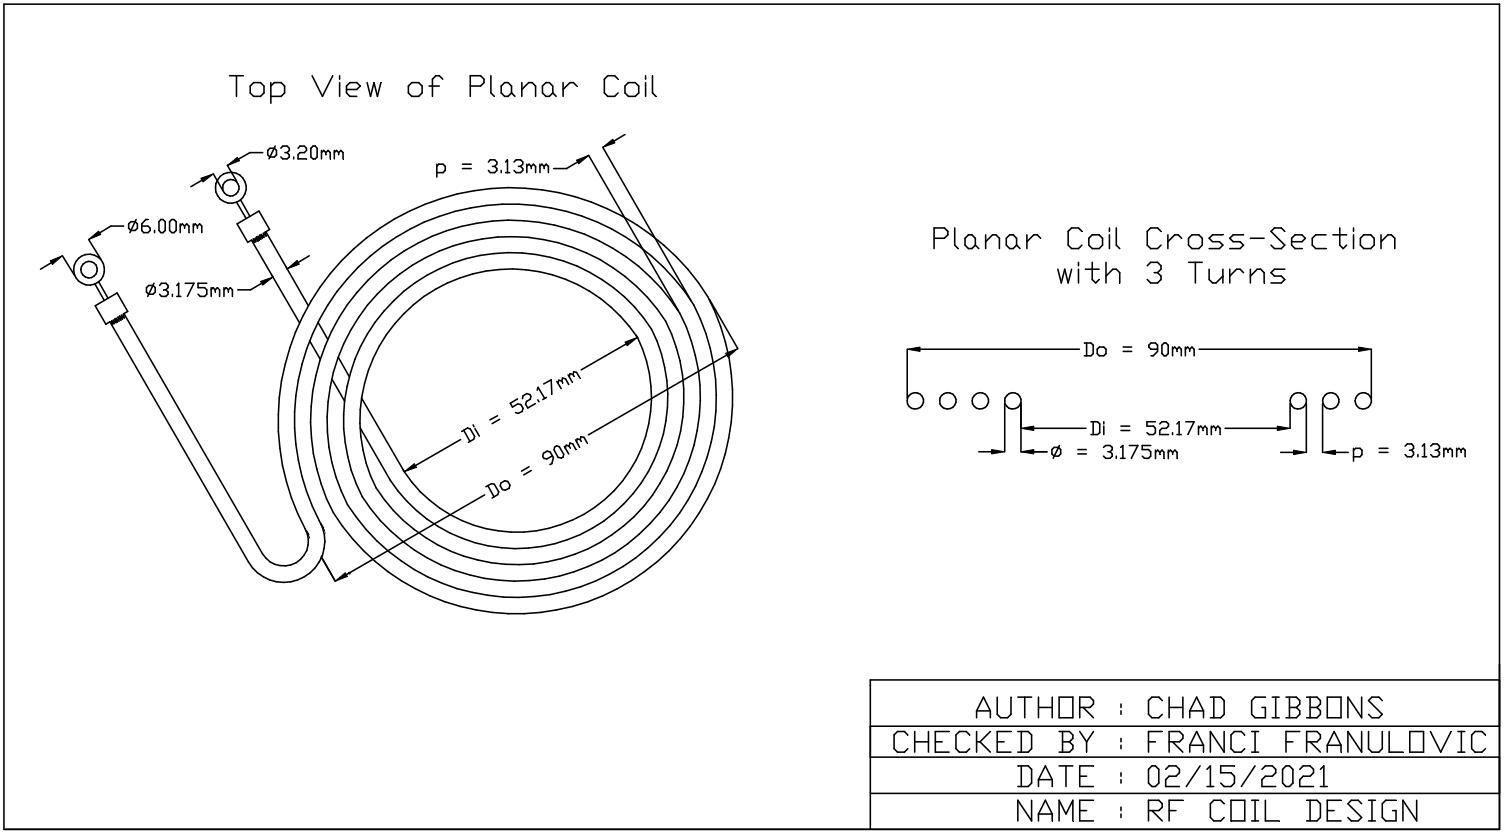
\includegraphics[width=0.95\linewidth]{Coil_CAD}
\caption{Planar Coil CAD Drawing}
\end{figure}

\hfill

\pagebreak

\subsection{Software Architecture}
\subsubsection{Firmware Architecture} The microcontrollers’ firmware architecture is split into two general categories: core functionality that is required for the microcontroller to operate and utilities that handle specific tasks that the microcontrollers need to complete.  The core functions primarily stem from interrupt calls and setup sequences.  The util functions will communicate through the bluetooth, display information, and handle or monitor power transmission.\\

\indent
Below is an example of the firmware architecture.
\hfill

\begin{figure}[h!]
\centering
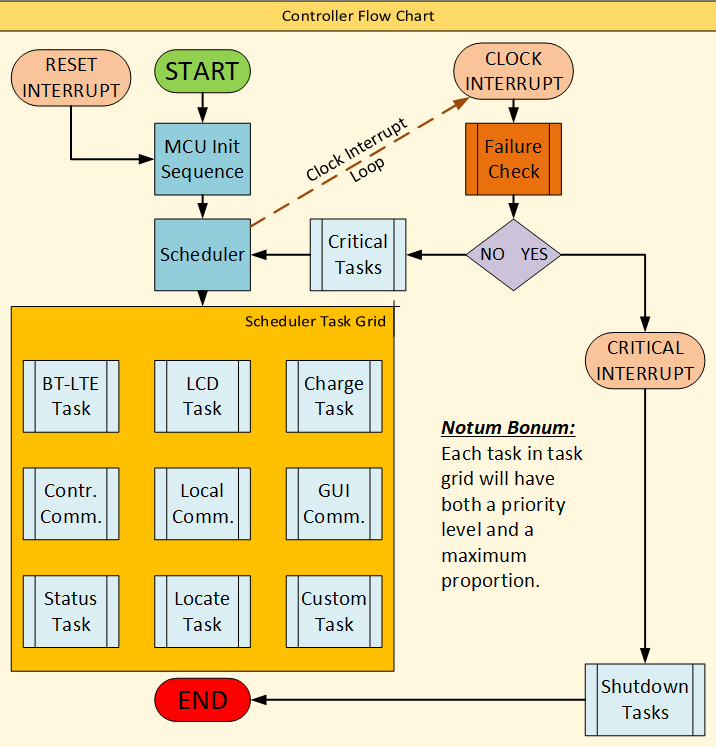
\includegraphics[width=0.88\linewidth]{mcu_workflow}
\caption{Controller Flow Chart}
\end{figure}

\hfill

\subsubsection{GUI Software Architecture} The GUI Software architecture is split into three general categories: Model, Controller, and View (MCV) components.  Each general category is then subdivided into layers of functionality to maintain modularity.  The Model is critical for handling data classes and storing data into files.  The Controller is responsible for operating the visual components and model objects.  The view category is utilized strictly for showing the graphical displays and are passive elements in the design’s architecture.\\

\indent
The figure below shows the GUI 's Model-Controller-View (MCV) Architecture
\hfill

\begin{figure}[h!]
\centering
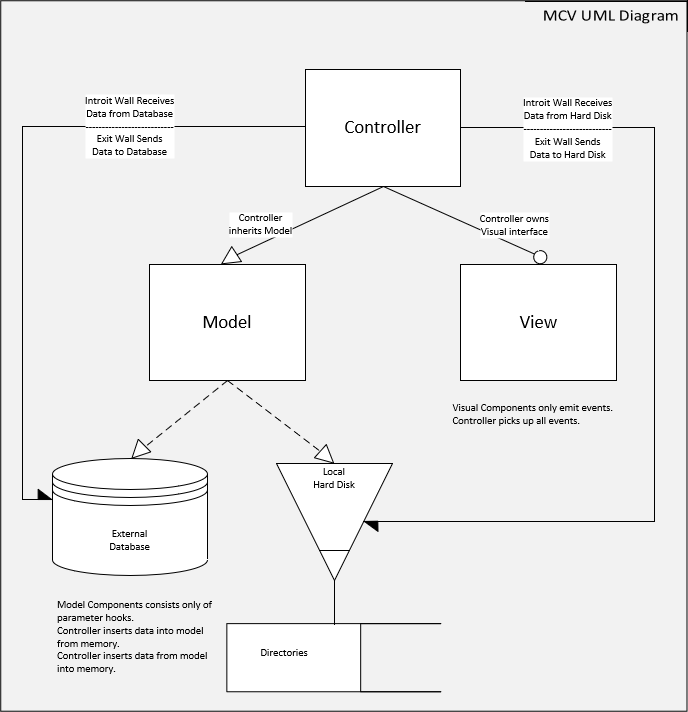
\includegraphics[width=0.88\linewidth]{mcv_arch}
\caption{High Level GUI Software Architecture Example}
\end{figure}

\hfill
\pagebreak

\subsection{Software Modules}

\subsubsection{Firmware Modules} \textit{Programmed on TI's Code Composer software and tested on TI's MSP430FR5994 Launchpad Kit}\\

\indent
* = confer to both header and C files.\\
%$\backslash$

\noindent
\textbf{
Microcontroller Setup \\
Location: 
}
\space Firmware$\backslash$MSP430FR5994\_MCU$\backslash$core$\backslash$mcu\_setup.*\\
\textbf{
Function: }
Activates port settings and instantiates utility functions that operate the program.\\

\noindent
\textbf{
Microcontroller Reset\\
Location: 
}
Firmware$\backslash$MSP430FR5994\_MCU$\backslash$core$\backslash$mcu\_reset.*\\
\textbf{
Function: }
Resets microcontroller to initial setup configuration.\\
 
 \noindent
\textbf{
Task Queue Scheduler\\
Location: 
}
Firmware$\backslash$MSP430FR5994\_MCU$\backslash$util$\backslash$Scheduler$\backslash$scheduler.*\\
\textbf{
Function: }
Creates and operates the scheduler method class that selects the next task to be run in the main loop based on task priorities. \\
 
 \noindent
\textbf{
Clock Interrupt\\
Location: 
}
Firmware$\backslash$MSP430FR5994\_MCU$\backslash$core$\backslash$Interrupts$\backslash$clock\_interrupt.*\\
\textbf{
Function: }
The code uses Timer A and SMCLK (1 MHz) to test clock interrupt. Once the program starts running, the timer counts up to 4 ticks to emit the clock interrupt signal every 250 ms period.  Additionally, it instantiates utility functions considered critical to repeat frequently.\\
 
 \noindent
\textbf{
Button Interrupt\\
Location: 
}
Firmware$\backslash$MSP430FR5994\_MCU$\backslash$core$\backslash$Interrupts$\backslash$button\_interrupt.*\\
\textbf{
Function: }
Four buttons are set up within a port. The code sets up an interrupt service routine to run when a button is pushed, so that their respective function is called. \\
 
 \noindent
\textbf{
Pin Input Voltage Reader \\
Location: 
}
Firmware$\backslash$MSP430FR5994\_MCU$\backslash$core$\backslash$Interrupts$\backslash$pins.*\\
\textbf{
Function: }
The function reads the analog 12 bit ADC input voltage at a port’s pin.\\
 
 \noindent
\textbf{
Communication Transmission\\
Location: 
}
Firmware$\backslash$MSP430FR5994\_MCU$\backslash$util$\backslash$Bluetooth$\backslash$bluetooth\_trans.*\\
\textbf{
Function: }
The code permits the transmitter to communicate directly with the receiver.  Alternatively, it permits the receiver to communicate with both the transmitter and a mobile device.\\
 
 \hfill
\pagebreak
\hfill

 \noindent
\textbf{
Communication Received \\
Location: 
}
\space Firmware$\backslash$MSP430FR5994\_MCU$\backslash$util$\backslash$Bluetooth$\backslash$bluetooth\_recv.*\\
\textbf{
Function: }
The code facilitates the reception and reaction to bluetooth messages received.  

\subsubsection{GUI Software Modules} \hfill \\
%\cross[0.4pt]\cross[0.4pt]\cross[0.4pt]

\noindent
\space \cross[0.4pt]\cross[0.4pt]\cross[0.4pt] = architecture layer ( Abstract - Base - Panel - Page - Window - App )\\
\space * = confer to both header and C++ files\\
 
 \noindent
\textbf{
Controllers\\
Location: }
Software$\backslash$controller$\backslash$\cross[0.4pt]\cross[0.4pt]\cross[0.4pt]\_controller.*\\
\textbf{
Function: }
The doer or agent component of the program.  Controllers allocate functions to particular events in the UI or manipulations to data models.\\
 
 \noindent
\textbf{
Widget Constructor\\
Location: }
Software$\backslash$controller$\backslash$widget\_setter.*\\
\textbf{
Function: }
The factory class that is dedicated to building widgets in a panel with the proper hierarchy of inheritance in order to give the controller mediate control of all widgets.\\
 
 \noindent
\textbf{
Bluetooth Low Energy\\
Location: }
Software$\backslash$core$\backslash$Bluetooth$\backslash$Protocols$\backslash$bt\_le.*\\
\textbf{
Function: }
The concrete method class handling Qt5 Bluetooth classes.\\
 
 \noindent
\textbf{
App Initialization\\
Location: }
Software$\backslash$core$\backslash$app\_init.*\\
\textbf{
Function: }
Configure all initial settings and ensure that the program is properly installed.\\
 
 \noindent
\textbf{
Models\\
Location: }
Software$\backslash$model$\backslash$\cross[0.4pt]\cross[0.4pt]\cross[0.4pt]\_model.*\\
\textbf{
Function: }
Data classes that can be pickled into compressed and encrypted binary data files.  These models provide the stable memory of the application.\\
 
 \noindent
\textbf{
Canvas\\
Location: }
Software$\backslash$ui$\backslash$CanvasTools$\backslash$\cross[0.4pt]\cross[0.4pt]\cross[0.4pt]\_canvas.*\\
\textbf{
Function: }
Concrete instances of Qt5’s QCanvas class for graphical displays of information.\\
 
 \noindent
\textbf{
Canvas Shapes\\
Location: }
Software$\backslash$ui$\backslash$CanvasTools$\backslash$\cross[0.4pt]\cross[0.4pt]\cross[0.4pt]\_canvas\_shape.*\\
\textbf{
Function: }
Individual images used as graphical displays of information and placed on their respective canvases.
\hfill
\pagebreak
\hfill
 
 \noindent
\textbf{
Panels\\
Location: }
Software$\backslash$ui$\backslash$Panels$\backslash$\cross[0.4pt]\cross[0.4pt]\cross[0.4pt]\_panel.*\\
\textbf{
Function: }
Concrete instances of movable panels used to hold widgets or canvases in GUI.\\
 
 \noindent
\textbf{
Toolbar Tools\\
Location: }
Software$\backslash$ui$\backslash$ToolbarTools$\backslash$win\_bar\_tools.*\\
\textbf{
Function: }
Flushes out available toolbar icons and functions.  Can also expand or limit drop down menu options at top of window.\\
 
 \noindent
\textbf{
Widgets\\
Location: }
Software$\backslash$ui$\backslash$Widgets\\
\textbf{
Function: }
Too many individual modules to account for in this document.  See GitHub repository \url{https://github.com/gibbs212521/HEC\_2_senior_design} for further detail.  These modules are Abstract-Concrete constructor classes that build their respective widgets with additional custom methods or attributes.\\
 
 \noindent
\textbf{
Windows\\
Location: }
Software$\backslash$ui$\backslash$Windows$\backslash$\cross[0.4pt]\cross[0.4pt]\cross[0.4pt]\_window.*\\
\textbf{
Function: }
Abstract-Concrete constructor classes that permit the appearance of various types of windows in the application (restricted in tablet/cellphone device compilation).\\
 
 \noindent
\textbf{
Power Monitor\\
Location: }
Software$\backslash$util$\backslash$power\_monitor.*\\
\textbf{
Function: }
Method class that ascertains whether the transmitter is sending power currently or not. Collects additional ancillary charging data.\\
 
 \noindent
\textbf{
Ticker Class\\
Location: }
Software$\backslash$ui$\backslash$Ticker$\backslash$\cross[0.4pt]\cross[0.4pt]\cross[0.4pt]\_ticker.*\\
\textbf{
Function: }
Collects or alters LCD ticker read out on the microcontroller.\\
 
 \noindent
\textbf{
App Configurations\\
Location: }
Software$\backslash$config.h\\
\textbf{
Function: }
Global variable module.  Ideally this file remains blank.\\
 
 \noindent
\textbf{
Application’s Hidden Settings\\
Location: }
Software$\backslash$.settings\\
\textbf{
Function: }
This file shall operate as a flat file to write or read current or most recent states in the application.\\
 
 \noindent
\textbf{
Main Program\\
Location: }
Software$\backslash$app.cpp\\
\textbf{
Function: }
The proverbial main.cpp that handles all dependencies of the application’s program.

\pagebreak

\subsection{Hardware Off The Shelf Items}

\indent \indent
The table below provides links and information on hardware incorporated in the post-production of the PCB.  Further information can be found in the BOM Appendices in Appendix C, D, and E.
%%%%% NOTE NEED TO INCLUDE LINE ABOVE IN WORD DOC
\hfill

\begin{table}[h!]
\centering
\caption{Off The Shelf Items Utilized in Prototype}
\begin{tabular}{ | l | l | l | }
\hline
Description [Name] & Part Number & Link\\
\hline
\parbox{0.3\linewidth}{\raggedleft Line Power Adapter: 65W 48V DC} & DT62PW480D  & 
\parbox{0.3\linewidth}{\raggedright  \url{https://product.tdk.com/en/search/power/switching-power/ac-dc-converter/info?part_no=DT62PW480D}}\\
\hline
74.52 Wh Li-Ion Battery & RRC RRC2040-2 & \parbox{0.3\linewidth}{\raggedright  \url{https://www.rrc-ps.com/en/battery-packs/standard-battery-packs/products/rrc2040-2/}}\\
\hline
LCD Display & NHD-0420DZ-FSW-FBW & \parbox{0.3\linewidth}{\raggedright  \url{https://www.newhavendisplay.com/specs/NHD-0420DZ-FSW-FBW.pdf}}\\
\hline
\end{tabular}
\end{table}

\hfill
\pagebreak
\hfill

\subsection{Software Off The Shelf Items}

\indent \indent
The table below includes all software used to develop hardware and the software for the wireless charger project.

\begin{table}[h!]
\centering
\caption{Off The Shelf Software Items}
\begin{tabular}{ | l | l | l | l | }
\hline
Name and Version & License Type & Restrictions & Link\\
\hline
\parbox{0.2\linewidth}{\raggedright  National Instruments Multisim 14.1} & Commercial & None & \parbox{0.3\linewidth}{\raggedright  \url{https://www.ni.com/en-us/shop/software/products/multisim.html}} \\
\hline
Altium 21.0.9 & Commercial & None & \parbox{0.3\linewidth}{\raggedright \url{https://www.altium.com/}}\\
\hline
Altium 365 & Commercial & None & \parbox{0.3\linewidth}{\raggedright \url{https://www.altium.com/altium-365}} \\
\hline
Gerbv 2.6A & GPL 2.0 & None & \parbox{0.3\linewidth}{\raggedright \url{http://gerbv.geda-project.org/}} \\
\hline
\parbox{0.2\linewidth}{\raggedright  Saturn PCB Design Inc. – PCB Toolkit ver.7.13} & \parbox{0.2\linewidth}{\raggedright  Commercial \\Freeware} & None & \parbox{0.3\linewidth}{\raggedright \url{ https://saturnpcb.com/pcb\_toolkit/}} \\
\hline
TI Code Composer & \parbox{0.2\linewidth}{\raggedright  Commercial \\Freeware} & None & \parbox{0.3\linewidth}{\raggedright \url{https://www.ti.com/tool/CCSTUDIO}} \\
\hline
Qt5 & LGPL 3 & \parbox{0.2\linewidth}{\raggedright Code must be Open Source and Free to Download}  & \parbox{0.3\linewidth}{\raggedright \url{https://doc.qt.io/qt-5/licensing.html}}\\
\hline
MS Visio & Personal License & No Corporate Use & \parbox{0.3\linewidth}{\raggedright  \url{https://www.microsoft.com/en-us/microsoft-365/visio/flowchart-software}} \\
\hline
NanoCAD & Personal License & No Corporate Use & \parbox{0.3\linewidth}{\raggedright \url{https://nanocad.com/products/nanoCAD/}} \\
\hline
GCC  & GPL 2.0 & None & \parbox{0.3\linewidth}{\raggedright \url{https://nanocad.com/products/nanoCAD/}} \\
\hline
\end{tabular}
\end{table}

\hfill
\pagebreak
\hfill

\subsection{Schematics / Wiring Diagrams / Technical Drawings}

\noindent
The schematics utilized can be found in appendices A and B with respect to the receiver, transmitter, and battery charger.\\

\noindent
The coil design and GUI wireframe can be found in appendices F and G.

\subsection{Custom Software}

\indent
All code is written modularly, to inspect functions or objects individually see repository of \url{https://github.com/ttgibbs212521/HEC\_2\_senior\_design}. \\

\subsubsection{Firmware Main Program} msp430\_proj.c\\

{\fontfamily{ptm}\ttfamily
\noindent
\#ifndef \_\_MC\_MSP430\_H\\
\#define \_\_MC\_MSP430\_H\\
\#include <msp430fr5994.h>\\
\#endif\\
\#include "util/Scheduler/scheduler.h"\\
\#include "core/mcu\_setup.h"\\
short main()\{\\
\indent mc\_setup();				// Setup Interrupts and Core Functions\\
\indent struct MCScheduler mc\_scheduler;	// Instantiate Scheduler Class Object\\
\indent buildScheduler(\&mc\_scheduler);	// Build Out Scheduler\\
\indent mc\_scheduler.run(\&mc\_scheduler);	// Begin Utility Function Loop\\
\indent return 1;		// Returns 1 since this point should never be reached\\
\}\\
}
\pagebreak

\subsubsection{GUI Software Main Program} app.cpp\\

{\fontfamily{ptm}\ttfamily
\noindent
\#include "Core$\backslash$app\_init.h"\\
\hfill \\
int main()\{\\
\indent AppController MotherController;\\
\indent MainWindow MainWin;\\
\indent AppModel PrimaryModel;\\
\indent MainWin.owner = \&MotherController; // use only for signaling\\
\indent PrimaryModel.owner = \&MotherController; // use only for signaling\\
\hfill \\
\indent AppController.getSettings(); // collect stable memory in .settings file\\
\indent AppController.setModel(\&PrimaryModel);  // giving control over model\\
\indent AppController.setUI(\&MainWin);  // giving control over window ui\\
\indent // AppController.setChildrenControllers()  // Currently only one page\\
\indent AppController.runApp();\\
\indent return 0;   // emits 0 on successful closure of application\\
\}
}


\hfill
\pagebreak
\hfill

\section{Prototype Design and Fabrication}
\subsection{Transmitter Subsystem Prototype Production}
\subsubsection{PCB Manufacturing} The transmitter boards are manufactured at JLC PCB  factory in China. The PCB specification shown below makes this board producible by many manufacturers because it does not require special manufacturing processes.\\

\noindent
For the fabrication process, Altium PCB CAD software is used to generate bord manufacturing files (Gerber X2).\\
 
\noindent
Gerber files include the following files:\\
Transmitter\_RevA\_Copper\_Signal\_Top.gbr          	\indent\space	TOP SIGNAL\\
Transmitter\_RevA\_Copper\_Plane\_1.gbr               	\indent\indent\space	GROUND PLANE\\
Transmitter\_RevA\_Copper\_Signal\_1.gbr  	        	\indent\indent	MID1 SIGNAL\\
Transmitter\_RevA\_Copper\_Signal\_Bot.gbr           	\indent\space	BOTTOM SIGNAL\\
Transmitter\_RevA\_Soldermask\_Top.gbr  	        	\indent\indent	TOP MASK\\
Transmitter\_RevA\_Soldermask\_Bot.gbr   	        	\indent\indent	BOTTOM MASK\\
Transmitter\_RevA\_Legend\_Top.gbr          	        	\indent\indent\indent\space	TOP SILK\\
Transmitter\_RevA\_Legend\_Bot.gbr           	        	\indent\indent\indent\space	BOTTOM SILK\\
Transmitter\_RevA\_Paste\_Top.gbr             	        	\indent\indent\indent\space\space\space	TOP PASTE\\
Transmitter\_RevA\_Paste\_Bot.gbr             	        	\indent\indent\indent\space\space\space	BOTTOM PASTE\\
 
\noindent
Reference Drill files\\
Transmitter\_RevA\_PTH\_Drill.gbr              	        	\indent\indent\indent\space\space	Plated through holes\\
Transmitter\_RevA\_NPTH\_Drill.gbr            	        	\indent\indent\indent	Non-plated through holes\\
 
 \noindent
NC DRILL\\
Transmitter\_RevA-RoundHoles.TXT         	        	\indent\indent\indent	N/C DRILL ROUND HOLES\\
Transmitter\_RevA-SlotHoles.TXT              	        	\indent\indent\indent\space\space\space	N/C DRILL SLOT HOLES\\
 
 \noindent
The transmitter boards are manufactured using the following specification:\\
 
 \noindent
Material: FR4 (135degC Tg) RoHS COMPLIANT\\
Board Thickness: 0.063"\\
Surface finish: Immersion Gold (Electroless Nickel Gold - ENIG)\\
Solder Mask Color: Green\\
Silkscreen Color: White\\
Min. Drill: 8 mils\\
Min. Line Width: 8 mils\\
Min. Spacing: 4 mils

 \hfill
 \pagebreak
 \hfill
 
 \noindent
The layers are stacked up as follows:\\
1. TOP SIGNAL\\
2. GROUND PLANE\\
3. MID1 SIGNAL\\
4. BOTTOM SIGNAL\\
 
 \noindent
The transmitter board size is  5.702 inches (144.821 mm) X 4.203 inches (106.76 mm).\\

\subsubsection{Transmitter Prototype Board Assembly} The group plans to assemble two transmitter boards. Parts for two boards are ordered using part numbers and quantities specified in the bill of materials. Quantities for small parts such as resistors, capacitors, some diodes, and some transistors are rounded to the nearest hundred because of the price break.\\

\indent
The assembly is performed manually using solder paste stencil and manual surface mount component placement. The solder paste stencil is custom made and is manufactured in the same facility as the PCB. Soldering is performed using a reflow oven. Through-hole parts are added after reflow oven soldering and soldered using standard solder pencil. All materials used in the assembly process are RoHS compliant.\\

\indent
For manual PCB assembly the group must provide detailed drawings of the PCB with visible reference designators, the bill of materials (BOM)  that includes components reference designators, component description, and part numbers.\\
 
\noindent
Required assembly documentation for the transmitter subsystem includes the following documents:\\
1. PCB Top silk layer and top copper layer drawings (c.f. Appendix B)\\
2. Bill of materials (c.f. Appendix D)\\

\hfill
\pagebreak
\hfill
 
 \indent
The figure below shows the PCB Top silk layer.

\begin{figure}[h!]
\centering
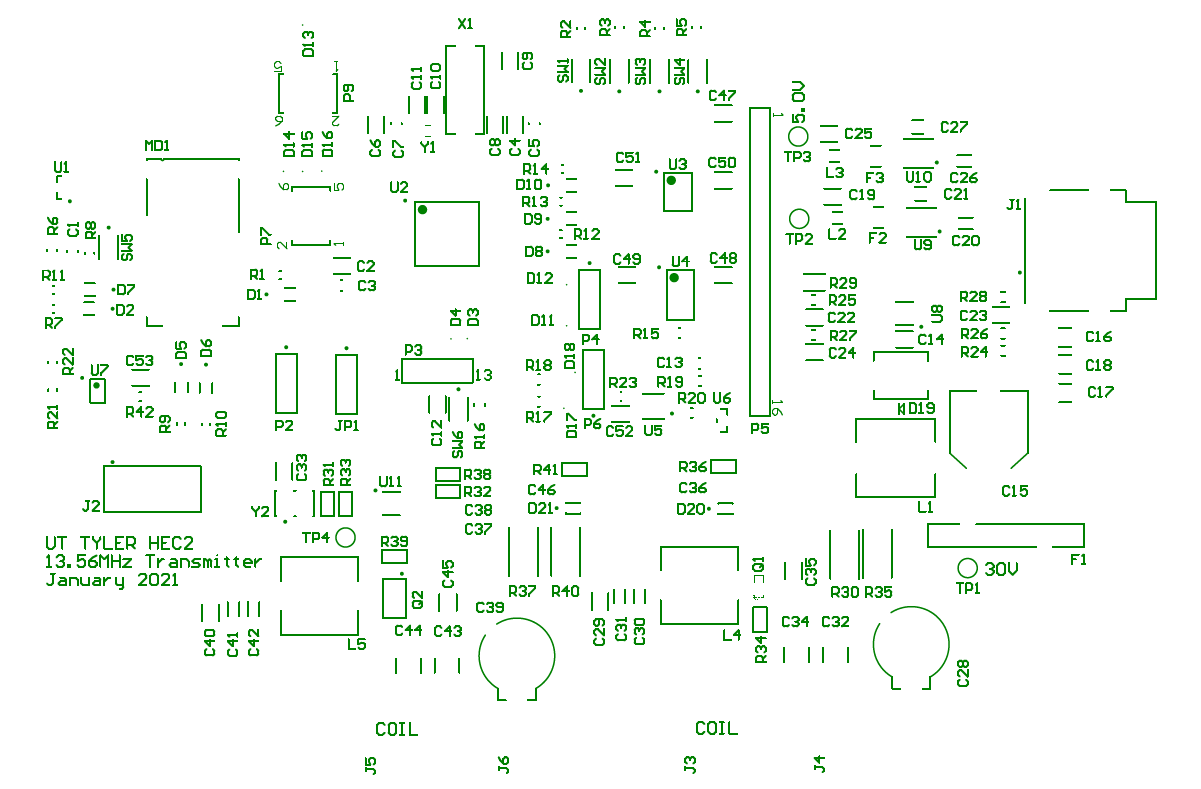
\includegraphics[width=0.75\linewidth]{tx_pcb_tslk}
\caption{Transmitter Top Silk Layer}
\end{figure}

The figure below shows the PCB Top copper layer.
\hfill

\begin{figure}[h!]
\centering
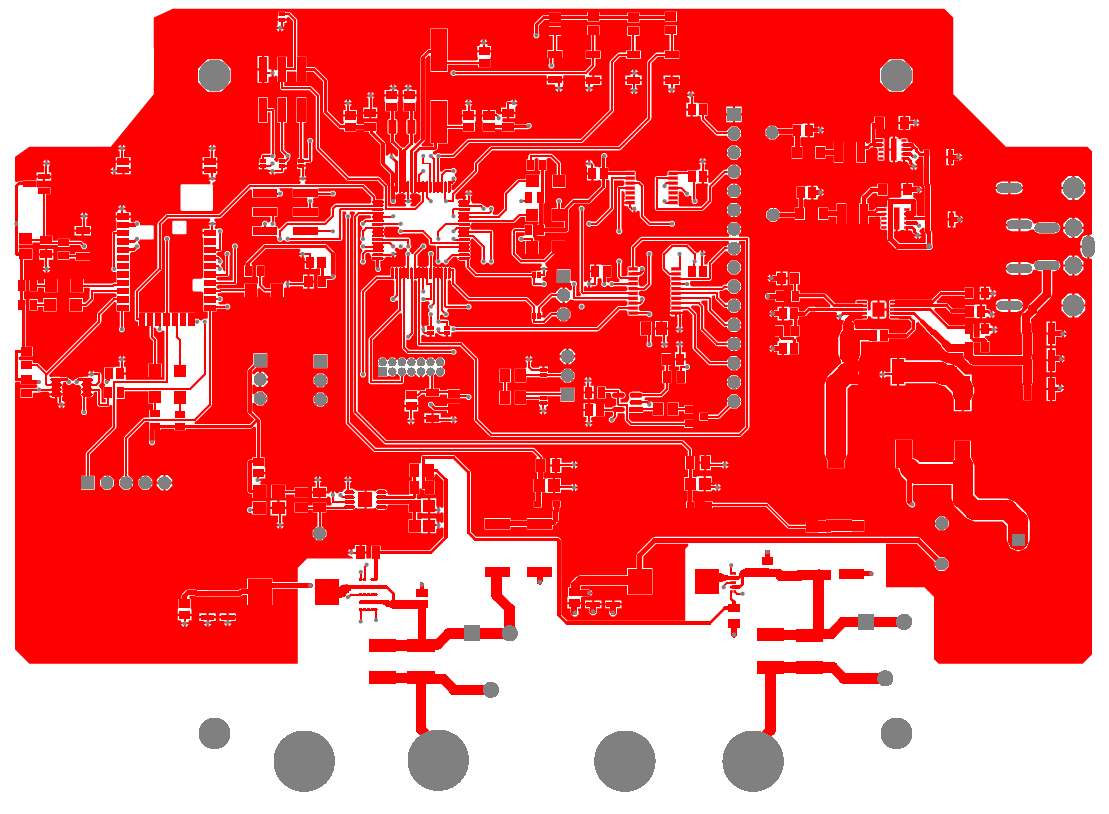
\includegraphics[width=0.75\linewidth]{tx_pcb_top_metal}
\caption{Transmitter Top Copper Layer}
\end{figure}

\hfill
\pagebreak
\hfill

\noindent
The assembly is performed by a professional worker. The assembly process consists of the following steps:\\
1.    Solder paste printing on the PCB\\
2.    Manual placement of surface mount components\\
3.    Soldering using a reflow oven.\\
4.    Through-hole soldering by hand using a solder iron pencil\\
 
 \noindent
All materials used in the assembly process are  RoHS compliant. Also, all tools used in this process are standard tools used for the PCB assembly process.

\subsubsection{Post Assembly Inspection}
After the boards are assembled they must be inspected for solder quality and possible assembly errors. Components values such as resistance, capacitance, and part numbers must be compared against the BOM and the board drawing. Also, the inspection step includes component polarity and solder quality inspection. After this step, the transmitter boards are ready for electrical verification and tests.\\

\indent
 The transmitter prototype design is intended to match the final hardware design. The enclosure selection may change depending on the thermal behavior of the transmitter subsystem. Also, the differences that may exist between the transmitter prototype and the final design solution are not known at this stage because the transmitter electronics performance and efficiency need to be validated. Depending on the test results the group may apply changes in the transmitter circuits.

\subsection{Receiver Subsystem Prototype Production}
\subsubsection{PCB Manufacturing} The receiver boards are manufactured at JLC PCB  factory in China. The PCB specification shown below makes this board producible by many manufacturers because it does not require special manufacturing processes.\\

\noindent
For the fabrication process, Altium PCB CAD software is used to generate bord manufacturing files (Gerber X2).\\
 
\noindent
Gerber files include the following files:\\
HEC2\_Receiver\_RevA\_Copper\_Signal\_Top.gbr          	\indent\space	TOP SIGNAL\\
HEC2\_Receiver\_RevA\_Copper\_Plane\_1.gbr               	\indent\indent\space	GROUND PLANE\\
HEC2\_Receiver\_RevA\_Copper\_Signal\_1.gbr  	        	\indent\indent	MID1 SIGNAL\\
HEC2\_Receiver\_RevA\_Copper\_Signal\_Bot.gbr           	\indent\space	BOTTOM SIGNAL\\
HEC2\_Receiver\_RevA\_Soldermask\_Top.gbr  	        	\indent\indent	TOP MASK\\
HEC2\_Receiver\_RevA\_Soldermask\_Bot.gbr   	        	\indent\indent	BOTTOM MASK\\
HEC2\_Receiver\_RevA\_Legend\_Top.gbr          	        	\indent\indent\indent\space	TOP SILK\\
HEC2\_Receiver\_RevA\_Legend\_Bot.gbr           	        	\indent\indent\indent\space	BOTTOM SILK\\
HEC2\_Receiver\_RevA\_Paste\_Top.gbr             	        	\indent\indent\indent\space\space\space	TOP PASTE\\
HEC2\_Receiver\_RevA\_Paste\_Bot.gbr             	        	\indent\indent\indent\space\space\space	BOTTOM PASTE

\hfill
\pagebreak
\hfill 

\noindent
Reference Drill files\\
HEC2\_Receiver\_RevA\_PTH\_Drill.gbr              	        	\indent\indent\indent\space\space	Plated through holes\\
HEC2\_Receiver\_RevA\_NPTH\_Drill.gbr            	        	\indent\indent\indent	Non-plated through holes\\
 
 \noindent
NC DRILL\\
HEC2\_Receiver.TXT         	        	\indent\indent\indent	N/C DRILL ROUND HOLES\\
 
 \noindent
The receiver board is manufactured using the following specification:\\
 
 \noindent
Material: FR4 (135degC Tg) RoHS COMPLIANT\\
Board Thickness: 0.063"\\
Surface finish: Immersion Gold (Electroless Nickel Gold - ENIG)\\
Solder Mask Color: Green\\
Silkscreen Color: White\\
Min. Drill: 8 mils\\
Min. Line Width: 8 mils\\
Min. Spacing: 4 mils\\
 
 \noindent
The layers are stacked up as follows:\\
1. TOP SIGNAL\\
2. GROUND PLANE\\
3. MID1 SIGNAL\\
4. BOTTOM SIGNAL\\

\noindent
The receiver board size is matching the enclosure recommended board dimensions.\\

\indent
The receiver prototype design is intended to match the final hardware design. The enclosure selection may change depending on the thermal behavior of the receiver subsystem. Also, the differences that may exist between the transmitter prototype and the final design solution are not known at this stage because the transmitter electronics performance and efficiency need to be validated and compared to the product specification. Depending on the test results the group may apply changes in the receiver circuits.
The receiver board size is  5.702 inches (144.821 mm) X 4.203 inches (106.76 mm).

\subsubsection{Receiver Prototype Board Assembly}

\indent
The group plans to assemble two receiver boards. Parts for two boards are ordered using part numbers and quantities specified in the bill of materials. Quantities for small parts such as resistors, capacitors, some diodes, and some transistors are rounded to the nearest hundred because of the price break. The assembly is performed manually using solder paste stencil and manual surface mount component placement. The solder paste stencil is custom made and is manufactured in the same facility as the PCB. Soldering is performed using a reflow oven. Through-hole parts are added and soldered after reflow oven soldering using standard solder pencil. All components and materials used in the assembly process are RoHS compliant.

\hfill
\pagebreak
\hfill

\indent
For manual PCB assembly the group must provide detailed drawings of the PCB with visible reference designators, the bill of materials (BOM)  that includes components reference designators, component description, and part numbers.\\
 
 \noindent
Required assembly documentation for the transmitter subsystem includes the following documents:\\
1. PCB Top silk layer and top copper layer drawings (ic.f. Appendix A)\\
2. Bill of materials (c.f. Appendix C)\\
 
 \indent
The figure below shows the PCB Top silk layer.

\begin{figure}[h!]
\centering
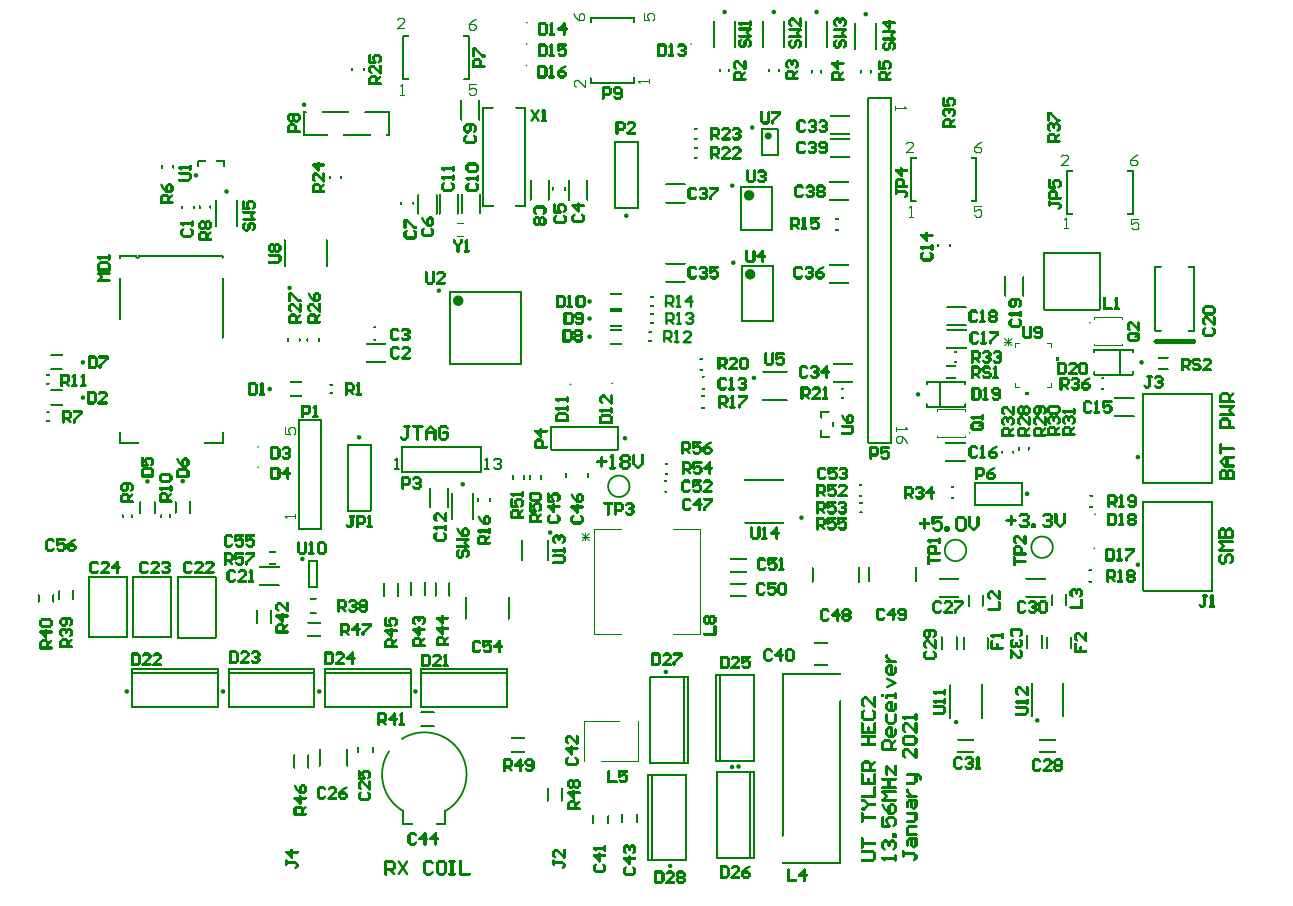
\includegraphics[width=0.88\linewidth]{rx_pcb_tslk}
\caption{Receiver Top Silk Layer}
\end{figure}

\hfill
\pagebreak
\hfill

\indent
The figure below shows the PCB Top copper layer.
\hfill

\begin{figure}[h!]
\centering
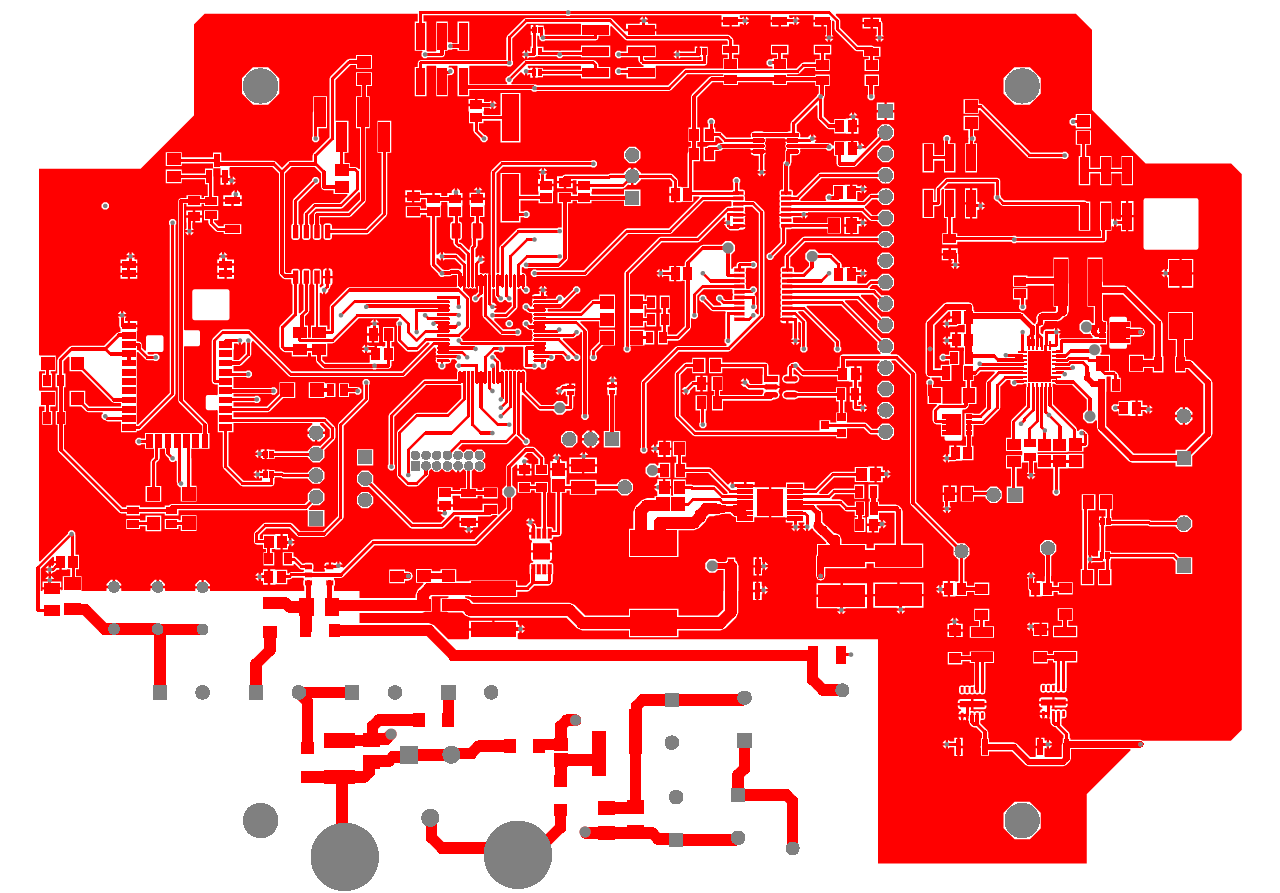
\includegraphics[width=0.75\linewidth]{rx_pcb_top_metal}
\caption{Receiver Top Copper Layer}
\end{figure}

\noindent
The assembly will be performed by a professional worker. The assembly process consists of the following steps:\\
 
 \noindent
1.    Solder paste printing on the PCB\\
2.    Manual placement of surface mount components\\
3.    Soldering using a reflow oven.\\
4.    Through-hole soldering by hand using a solder iron pencil\\
 
 \noindent
All materials used in the assembly process are  RoHS compliant. Also, all tools used in this process are standard tools used for the PCB assembly process.
 
 \subsubsection{Post Assembly Inspection}

\indent
After the boards are assembled they must be inspected for solder quality and possible assembly errors. Components values such as resistance, capacitance, and part numbers must be compared against the BOM and the board drawing. Also, the inspection step includes component polarity and solder quality inspection. After this step, the receiver boards are ready for electrical verification and tests.\\
 
 \indent
The receiver prototype design is intended to match the final hardware design. The enclosure selection may change depending on the thermal behavior of the receiver subsystem. Also, the differences that may exist between the receiver prototype and the final design solution are not known at this stage because the receiver electronics performance and efficiency need to be validated. Depending on the test results the group may apply changes in the receiver circuits.
\hfill
\pagebreak

\subsection{Coil Production}

\indent \indent
The coil development process involves printing a 3-dimensional hollow plastic fixture. The interior of the fixture contains a spiral bas-relief that shall fix the coil in the specified spiral form. The coil shall be connected to the PCB board using stranded copper wire. For ideal performance conditions, the coil must withstand 600V rms as well as possess a resistance of 69.906 m$\Omega$. The coil is encased in a plastic enclosure to prevent electric shock. The plastic enclosure specification will have a size of 130mm x 110mm x 20mm. MFG alpha rated wire will be soldered to the coil and the other end of wire will be terminated with the ring terminal.  

\subsection{Expenditure Report}

\indent \indent
The list below shows development tools and assembly tools cost that are used as an aid to design and produce the wireless charger system. This list does not include the cost of components that are part of the system.\\

\noindent
\textbf{Evaluation Kits for Firmware}\\

\noindent
Bluetooth Development Tools (802.15.1) RN4870 Sensor Board \\
Manufacturer part number: RN-4870-SNSR\\
Mouser part number: 579-RN-4870-SNSR\\
Cost: \$91.80\\
Ordered: 1 unit\\
Total cost: \$91.80\\

\noindent 
Bluetooth Development Tools (802.15.1) RN4870 click\\
Manufacturer part number: MIKROE-2543\\
Mouser part number: 932-MIKROE-2543\\
Cost: \$33.00\\
Ordered: 3 units\\
Total cost \$99.00\\

\noindent
Development Boards \& Kits - MSP430 MSP430FR5994 LaunchPad Dev Kit\\
Manufacturer part number: MSP-EXP430FR5994\\
Mouser part number: 595-MSP-EXP430FR5994\\
Cost: \$20.39\\
Ordered: 5 units\\
Total cost \$101.95

\hfill
\pagebreak
\hfill

\noindent
\textbf{Hardware Evaluation Kits}\\

\noindent
Power Management IC Development Tools LTC4162 DC2038= Li-ion,adjustable, MPP\\
Manufacturer part number: DC2038A-J\\
Mouser part number: 584-DC2038A-J\\
Cost: \$150.00\\
Ordered: 1 unit\\

\noindent
Battery packs for charger controller testing\\
Battery Packs 11.1V, 6.4Ah, 72Wh battery (3s2p)\\
Manufacturer part number: RRC2040-2\\
Mouser part number: 328-RRC20402\\
Ordered: 1 unit\\
Cost: \$105.00\\

\noindent
\textbf{Solder Stencil Production}\\

\noindent
Solder paste stencils are ordered for each subsystem.\\
Manufacturer: JLC PCB\\
Manufacturer part number: Custom order\\
Solder paste stencil \$7.05\\
Total cost \$14.10

\hfill

\begin{table}[h!]
\centering
\caption{Summary of Expenditures}
\begin{tabular}{ | c | l | l | r | }
\hline
 & Expenditure Description &  Subsystem & Cost\\
\hline
1 & Hardware development kits & Receiver & \$255.00\\
\hline
2 & Firmware evaluation kits & Transmitter/ Receiver & \$226.75\\
\hline
3 & Solder paste stencils (board assembly) & Transmitter/Receiver & \$14.10\\
\hline 
 & TOTAL COST &  & \$495.85\\
\hline
\end{tabular}
\end{table}

\hfill
\pagebreak
\hfill

\indent
The tables below account for man-hours expended in development and prototyping.
\hfill

\begin{table}[h!]
\centering
\caption{Man-Hours Expenditure Report in Development and Prototyping}
\begin{tabular}{ | r | c | }
\hline
\hline
Task Description & Man-Hours \\
\hline
\hline
\hline
\textbf{Coil Production} & \\
\hline
Francsico Sosa worked on coil & 8 \\
\hline
Franci Franulovic worked on coil & 8 \\
\textbf{Subtotal} & \textbf{16 hours}\\
\hline
\hline
\textbf{Schematic design and capture} & \\ 
\hline
 David Flory & 90  \\
 \hline
 Franci Franulovic  & 12 \\
 \hline
\textbf{Subtotal} & \textbf{102 hours}\\
\hline
\hline
\textbf{PCB Layout Design} & \\
 \hline
Franci Franulovic & 10\\
 \hline
David Flory & 9 \\
 \hline
\textbf{Subtotal} & \textbf{19 hours}\\
\hline
\hline
\textbf{PCB Assembly} & \\
 \hline
Estimated time required to assemble four prototypes & 16 \\
 \hline
\textbf{Subtotal} & \textbf{16 hours}\\
\hline
\hline
\textbf{Post Assembly Inspection } & \\
 \hline
Assembly verification & 1 \\
 \hline
Solder quality inspection & 1 \\
 \hline
\textbf{Subtotal} & \textbf{2 hours}\\
\hline
\hline
\textbf{GUI Software Development} & \\
 \hline
Chad Gibbons on GUI Software Architecture & 5\\
 \hline
Chad Gibbons & 2 \\
 \hline
\textbf{ Subtotal} & \textbf{7 hours}\\
\hline
\hline
\textbf{Firmware development } & \\
 \hline
Natasha Franca & 25\\
 \hline
 Francisco Sosa & 8\\
 \hline
 Chad Gibbons & 32\\
 \hline
Chad Gibbons worked on test suite & 10\\
 \hline
\textbf{Subtotal} & \textbf{75 hours}\\
\hline
\end{tabular}
\end{table}

\hfill
\pagebreak
\hfill

\begin{table}[h!]
\centering
\caption*{Man-Hours Report Continued}
\begin{tabular}{ | r | c | }
\hline
\hline
\textbf{Task Description} & \textbf{Man-Hours}\\
\hline
\hline
\hline
\textbf{Learning Curves and Used Skilled Resources} & \\
 \hline 
David Flory on Altium &  7 \\
 \hline
Firmware Team studied C/C++ & 15 \\
 \hline
Franci Franulovic developed PCB Schematic Drawing & 11 \\
 \hline
Natasha Franca learned Object Oriented Programming in C & 2 \\
 \hline
\textbf{Subtotal} & \textbf{35 hours}\\
\hline
\hline
\textbf{Subsystem Prototyping} & \\
 \hline 
Receiver PCB assembly & 8 \\
 \hline
Parts procurement & 2 \\
 \hline
Coil assembly  & 8\\
 \hline
Coil Test & 5 \\
 \hline
Hardware test & 17 \\
 \hline
Firmware test & 6\\
 \hline
Quality control inspection & 8 \\
\hline
\textbf{Subtotal} & \textbf{54 hours} \\
\hline
\end{tabular}
\end{table}

\hfill 

\begin{table}[h!]
\centering
\caption{Development and Prototyping Summary of Man-Hours}
\begin{tabular} { | r | c | }
\hline
\textbf{Task Description} & \textbf{Man-Hours} \\
\hline
Time Learning & 35\\
\hline
Software Development & 82 \\
 \hline
Hardware Development & 137 \\
 \hline
Assembly & 36\\
 \hline
Quality Assurance & 36\\
 \hline
\textbf{Total} & \textbf{326 hours}\\
\hline
\end{tabular}
\end{table}

\hfill
\pagebreak
\hfill

\subsection{Budget}

\indent \indent
This budget lists the expenses for development hardware, prototyping materials, and skilled labor necessary to realize and test the prototype.

\hfill
\begin{table}[h!]
\centering
\caption{Development and Prototyping Budget}
\begin{tabular}{ | l | l | c | r | }
\hline
\textbf{Item Description} & \textbf{Price} & \textbf{Qty.}  & \textbf{Totals}\\
\hline
Microchip Bluetooth RN4870 Sensor Board & \$91.80 & 1 & \$91.80\\
\hline
Mikroe Bluetooth RN4870 click & \$33.00 & 3 & \$99.00\\
\hline
TI MSP430FR5994 LaunchPad Dev Kit & \$20.39 & 5 & \$101.95\\
\hline
Analog Devices LTC4162-L Evaluation Board & \$150.00 & 1 & \$150.00\\
\hline
RRC Battery Packs 11.1V, 6.4Ah, 72Wh battery (3s2p) & \$105.00 & 1 & \$105.00\\
\hline
16x2 Parallel LCD Display (for evaluation) & \$20.63 & 3 & \$61.89\\
\hline
Receiver BOM & \$77.30 & 2 & \$154.59\\
\hline
Transmitter BOM & \$128.78 & 2 & \$257.55\\
\hline
System BOM & \$136.92 & 1 & \$136.92\\
\hline
 &  &  & \\
\hline
\textbf{Total Hardware} &  &  & \textbf{\$1,158.70}\\
\hline
\end{tabular}
\end{table}

\hfill
\pagebreak
\hfill

\subsection{Current Manufacturing Abilities}

\indent \indent
The process starts with the purchase of the necessary components. Having the PCBs’ Altium CAD Software drawings, the transmitter and receiver board files are sent for manufacturing at JLC PCB factory in China. Shipping time for the boards are around seven days. Small parts for the boards are also generated in the Altium software as a bill of materials, and those include but are not limited to resistors, capacitors, transistors, and diodes. Those can be ordered anywhere online and take up to seven days for delivery. Small parts can be purchased at local electronics stores. Hardware off-the-shelf items include power adapter, Li-Ion battery, and LCD display, and those can also be readily purchased at any local electronics store. Assembling is done by soldering the components according to the board layout, and each board takes approximately four to five hours to assemble by hand. The last setup step is to load the firmware onto the boards which requires less than one hour. In that same hour, testing the prototype can be completed if there are no issues hindering the charging process. The board would need to be troubleshooted for firmware, software, or hardware issues; the troubleshooting can take minutes or hours to fix.  

\begin{table}[h!]
\centering
\caption{Prototype Production Timetable}
\begin{tabular}{ | l | l | }
\hline
\textbf{Description} & \textbf{Time Required}\\
\hline
Shipping Time for PCBs and other components & 7 days\\
\hline
Manual receiver PCB assembly & 5 hours\\
\hline
Manual transmitter PCB assembly & 5 hours\\
\hline
Parts procurement process for each subsystem & 2 hours\\
\hline
Coil assembly for each subsystem & 1 hour\\
\hline
Coil Test & 1 hour\\
\hline
Hardware test & 1 hour\\
\hline
Firmware load and test & 1 hour\\
\hline
Quality control inspection & 8 hours\\
\hline
\textbf{Total} & \textbf{8 days} \\
\hline
\end{tabular}
\end{table}

\hfill
\pagebreak
\hfill

\section{Testing and Validation}
\indent
Validation of a product prototype is an important step to determine the performance, reliability, and durability of the designed product. Without proper testing, the product life cycle can be severely limited due to component failure or subcircuit malfunction.  All basic functionality for each subsystem is verified by following standard test practices. The transmitter and receiver subsystems were subjected to validation tests described below to observe their actual performance. 

\pagebreak

\section*{Transmitter Tests} %%%%%%%%%%%%%%%%%%%%%%%%%%%%%%%%%%%%%%%%%%%%%%%%%
\subsection{Transmitter Power Supply Tests}
\indent
The transmitter prototype board testing starts by applying DC voltage on pins 3, and 4 positive terminals and pins 1-7 negative terminals. DC voltage is supplied using a bench power supply with the current limit set to 0.3A. The power supply voltage is gradually increased from 0V to the nominal voltage of 48V while the bench power supply current was constantly monitored.
The 30V regulator will start regulating if the input voltage is higher than 38.3V. The expected output voltage on TP 1 is 30V +/-2\% due to reference voltage tolerance and resistors used for setting the output voltage.\\

\noindent
After the 30V regulator test, the voltage output is verified the following low voltage regulators are verified:\\
\hfill \\
\indent \indent $\cdot$ 3.3V regulator (U11) test point TP2 nominal voltage 3.3V  tolerance +/- 1.5\% \\
\indent \indent $\cdot$ 5V regulator (U11) test point TP3 nominal voltage 5V  tolerance +/- 1.5\%\\

\noindent
Below is the part of the schematic diagram showing test points TP1, TP2, and TP3.
\hfill
\begin{figure}[h!]
\centering
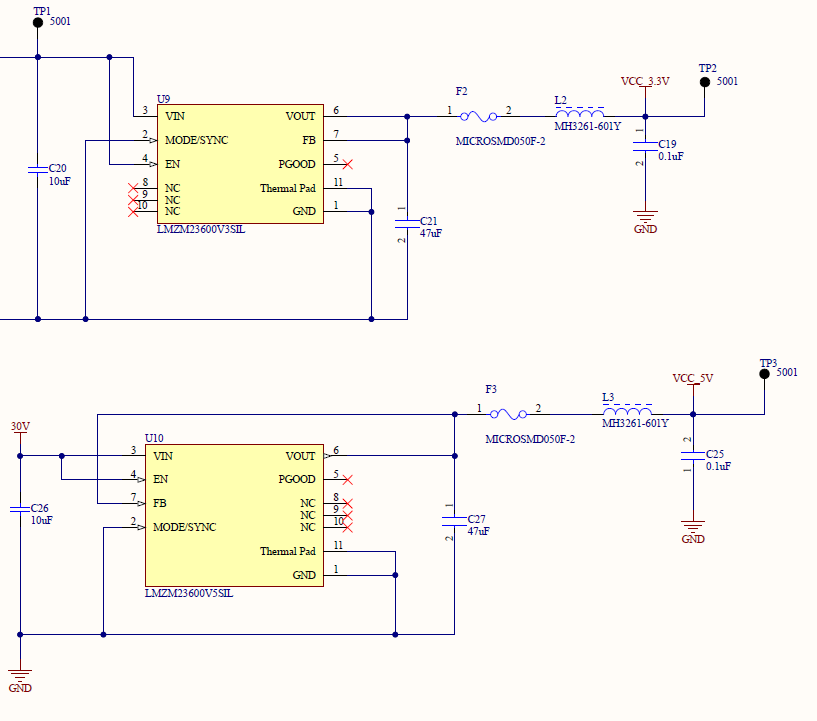
\includegraphics[width=0.82\linewidth]{Transmitter_power_supply_sch_diag}
\caption{Transmitter Voltage Regulator Circuits}
\end{figure}

\hfill \\
\indent
After power modules are verified the test firmware can be loaded using a JTAG connection on the board.  The firmware sets all parameters in the default state for testing. The coil driver is disabled and all peripherals are turned off.

\subsection{Transmitter Coil Driver Tests}
\indent
After the firmware is loaded the board is turned off and the transmitter coil is connected to the terminals J3 and J4. The coil driver circuit is tested using a variable voltage supply. To perform this test PPTC fuse, F1 is removed and the bench power supply is connected to the TP1 (positive terminal) and the negative terminal is connected to the ground.  The oscilloscope probe is attached to the drain of  Q1 (GaN FET transistor).  The second probe is connected to the output of the 13.56MHz temperature compensated oscillator (TP4).\\

\indent
After the test equipment is attached the power supply is turned on and the output voltage is gradually increased. When the power supply is higher than 5V voltage regulators (3.3V and 5V) are enabled and they provide power to the transmitter subcircuits.  The temperature compensated oscillator (TXCO) enable line is controlled by push buttons. When the oscillator enable line is set to a high level a 13.56MHz signal is enabled and 13.56MHz is fed into the Class E amplifier driver (U11). The expected voltage from the TXCO on TP4 is 3.3Vpp.  After the oscillator subcircuit is verified the oscilloscope probe is placed on one of the terminals of jumper R32 to verify the functionality of U11. The expected amplitude on the output of the Class E amplifier driver is 5Vpp.\\

\noindent
The figure below presents the subcircuit wherein the transmission signal is generated and tested.
\hfill
\begin{figure}[h!]
\centering
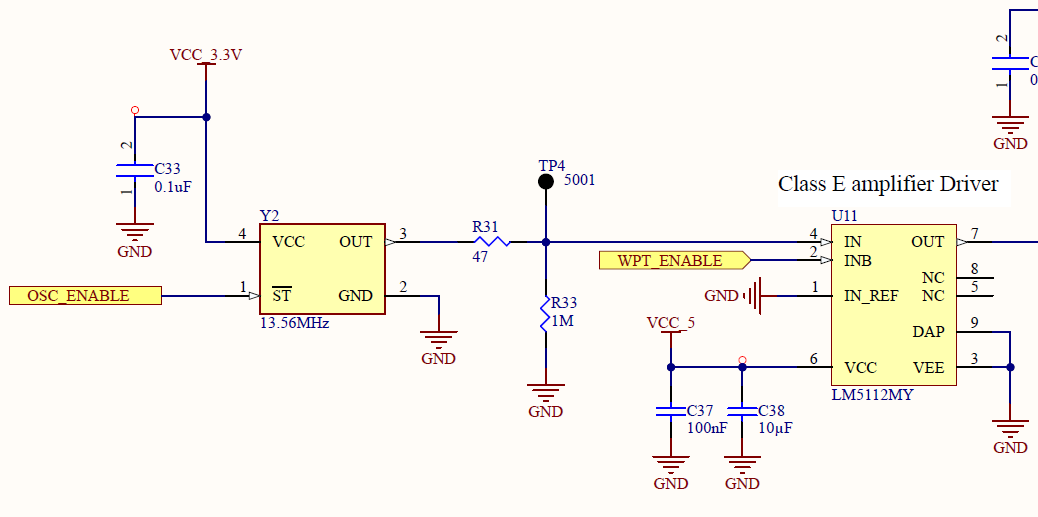
\includegraphics[width=0.9\linewidth]{TX_oscillator_and_buffer}
\caption{Oscillator and Buffer Subcircuit}
\end{figure}
\hfill \\
\pagebreak

\indent
The GaN FET switching is verified by observing the GaN FET drain voltage waveform that will have a voltage swing from 0V to 117V if the power supply voltage is set to 30 V. For lower supply voltages the swing will be lower but it always should swing from 0V to some positive voltage.  After the GaN FET switching is verified the transmitter coil resonance will be adjusted. \\

\indent
To set transmitter coil resonance a variable capacitor (C28) must be adjusted while the voltage across the coil is monitored using a 100X oscilloscope probe attached to J4  (transmitter board coil terminal). The trimmer capacitor must be adjusted until the voltage across the transmitter coil reaches the maximum value. After the resonance is achieved the power supply voltage is gradually increased to 30V while the supply current is constantly monitored.  The expected voltage on the drain of the GaN FET is 117Vpp. The measured voltage is recorded.  The 30V power supply current should be 120mA if there is no load present (no receiver coil in the front of the transmitter coil).\\

\noindent
The figure below presents the subcircuit wherein the transmission signal is amplified and observed by a Class E amplifier.
\hfill
\begin{figure}[h!]
\centering
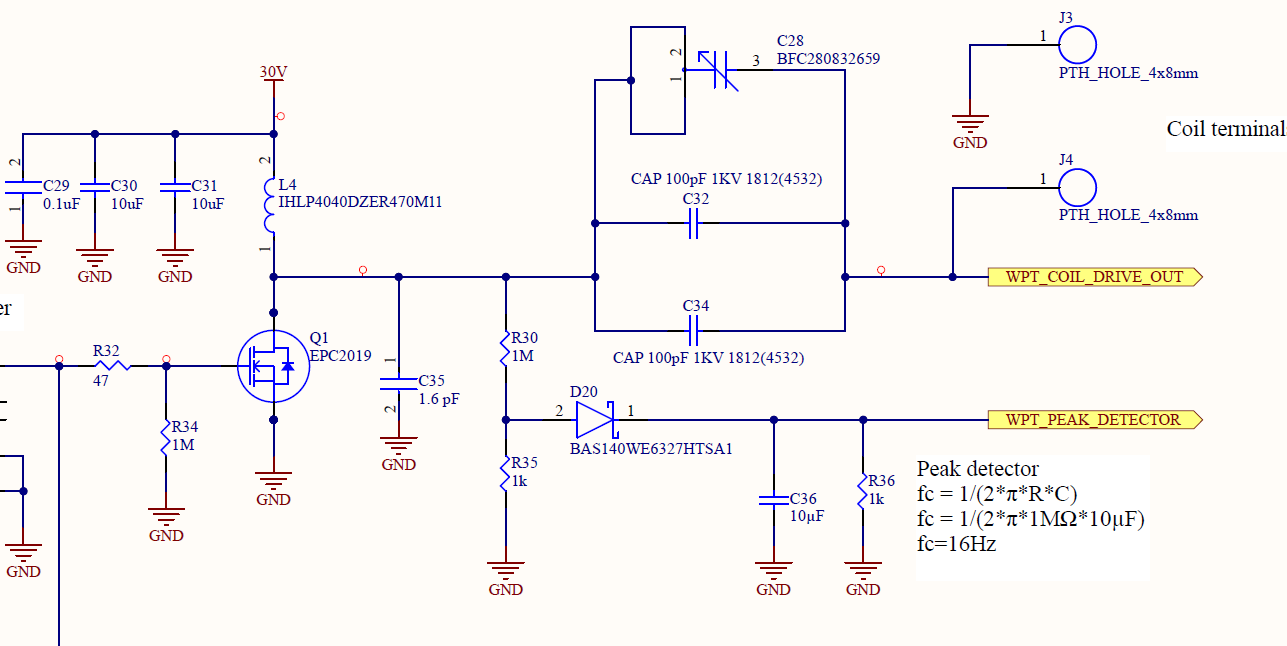
\includegraphics[width=0.9\linewidth]{Class_E_amplifier}
\caption{Transmission Signal Class E Amplifier Subcircuit}
\end{figure}
\hfill \\
\pagebreak
\hfill \\
\indent
Transmitter power output is measured when the class E amplifier is verified and the amplifier power supply voltage is 30V.  The specified transmitter power output is 30W. The power output is measured by placing receiving LC circuit loaded with a 50Ω high power resistor in the front of the transmitter coil at a distance of 5 cm. The peak to peak voltage across the load is measured using the oscilloscope and recorded in the table. This process is repeated for distances of 4 cm, 3 cm, 2 cm, and 1 cm.
\hfill
\begin{figure}[h!]
\centering
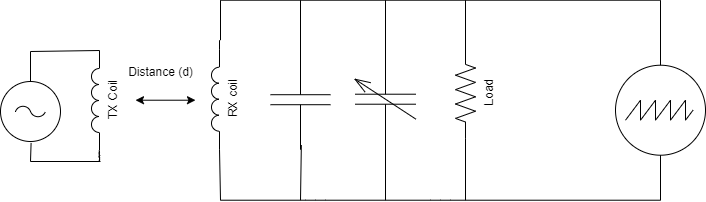
\includegraphics[width=0.75\linewidth]{Variable_RX-TX_Distance}
\caption{Received Power vs. Distance Test Setup}
\end{figure}

\subsection{Transmitter Firmware Tests}

\noindent
The figure below is a reference for the transmitter part numbers and pin numbers.  The part numbers can be found adjacent to the part outline with a prefix of P, J, U, Q, F, D, R, C, or L.  Pin numbers are found without a prefix adjacent to the first and last pin with their respective number in any part denoted by the prefix P where space provides.
\hfill
\begin{figure}[h!]
\centering
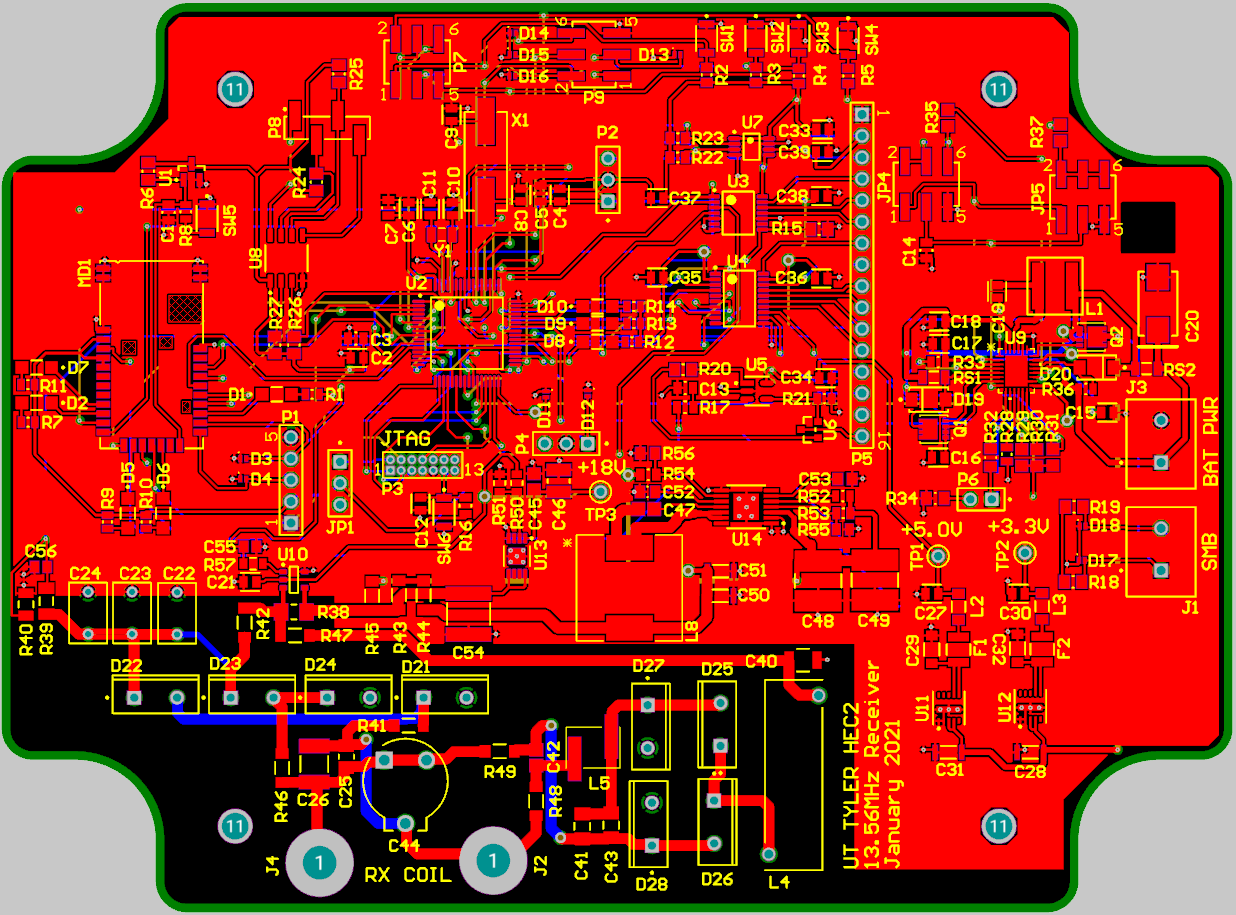
\includegraphics[width=0.8\linewidth]{receiver_pcb_layout}
\caption{Reference Layout for Part and Pin Numbers}
\end{figure}

\hfill
\pagebreak
\hfill 
\subsection{Transmitter Firmware Tests}

\indent
The first recommendation in any trouble rise of troubleshooting of quality assurance is to check the mcu\_setup.c and mcu\_setup.h files.  Additionally, it is good to note that a unit test is a type of software test that only requires building a small portion of the codebase in order to test a set of specific modules.  Unit testing reduces the total amount of time dedicated into the development of any software.

%%% Currently at once every two seconds
\subsubsection*{The MCU Clock On LED} (MCU\_Clock\_on or D8 by the microcontroller) should be blinking at a rate of approximately twice every second \textbf{(This rate is subject to change)}.  If this is not occurring, the clock interrupt routine is not operating properly.  Investigate for over-polling at the UART RX Pins (P2.0 and P2.5) is occurring.  Alternatively, the TX Pins could be written out of turn (P2.1 and P2.6) which would thus initiate the UART Interrupts EUSCI\_A0\_VECTOR (located at P2.0 and P2.1) or EUSCI\_A1\_VECTOR (located at P2.5 and P2.6).  If this is not the case, the next step would be to troubleshoot the ADC (Analog to Digital Converter) Pins (P3.0, P3.1, P3.2, and P3.3).  If this issue where the ADC12\_B\_VECTOR interrupt contravenes the clock interrupt is detected, the error is likely caused by a breakdown in the hierarchy of interrupts.  In such a case, the code must be provided additional logic on how to handle specific interrupts in the scheduler’s run method.

\subsubsection*{The LCD Ticker Panel} should display some coherent statement or acronym.  If it does not, running of a “Hello World” unit test to the LCD is required for appropriate troubleshooting.  The unit test should utilize the identical function used in the production code.  If the unit test passes without errors, the error would reside in the accumulation of text that is meant to be passed into the LCD Ticker Panel.

\subsubsection*{The UART (RX/TX) CON} tests require unit tests. There are four unit tests to be done to test the non-Bluetooth UART ports (P2.5 and P2.6).  The first involves transmitting a ‘A’ character to the same PCB’s RX\_CON Pin (P2.5).  The next unit test would involve transmitting a string and acknowledgement TCP handshake.  These same unit tests are repeated with a secondary PCB.

\subsubsection*{The Bluetooth} validation tests will involve a unit test from the personal computer that connects to the receiver and sweeps through a set of pre-programmed unit tests that provide specific responses and sample data points.

\subsubsection*{The Wireless Power Transmission (WPT) Signal Generation} test should be conducted prior to connecting the transmitter's WPT coil.  Press Button 0 at SW1 to turn on the signal generator and measure the voltage at the transmitter WPT Coil Junction points (J3 with J4 as well as J5 with J6).  Once the voltage is observed, press Button 1 at SW2 to turn off the signal generator, and a drop off of voltage should be observed. \textbf{(NOTE: The button closest to the microcontroller is Button 0 while the button furthest from the microcontroller and closest to the pins of Part P5 is Button 4. The buttons are arranged in sequential order.)}
%%%%%%%%%%%%%%%  NEED WPT_PEAK_DETECTOR Algorithm
\hfill
\pagebreak
\section*{Receiver Tests}  %%%%%%%%%%%%%%%%%%%%%%%%%%%%%%%%%%%%%%%%%%%%

\subsection{Receiver Power Supply Tests}
\indent
The receiver prototype board testing starts by applying DC voltage across coil terminals for power supply verification at the Receiver Coil Junction Points (J2 and J4).  The Coil terminal subcircuit is shown in the figure below.
\hfill
\begin{figure}[h!]
\centering
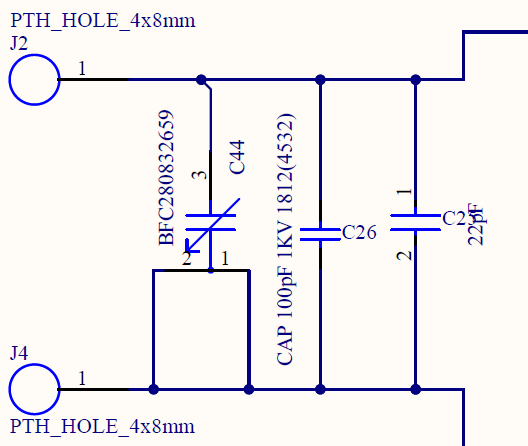
\includegraphics[width=0.75\linewidth]{RX_COIL_TERMINALS}
\caption{Receiver Coil Terminal Subcircuit}
\end{figure}
\hfill \\
\indent
This test is necessary for determining whether the voltage regulators output voltages are matching the design specification.\\

\noindent
The following voltage regulators are verified in this test:
\indent \indent $\cdot$3.3V regulator (U12) test point TP2 nominal voltage 3.3V  tolerance +/- 1.5\%\\
\indent \indent $\cdot$5V regulator (U11) test point TP1 nominal voltage 5V  tolerance +/- 1.5\%\\
\indent \indent $\cdot$18V regulator (U13A) test point TP3 nominal voltage 18V tolerance +/- 2\%\\

\noindent
After power module verification the test firmware can be loaded using a JTAG connection on the board.  The firmware sets all parameters in the default state for testing.

\hfill \\
\pagebreak

\subsection{Receiver Wireless Power Rectifier Tests}

\noindent
Specification  for AC-DC (RF-DC) conversion efficiency is 80\%\\
 
\noindent
Conversion efficiency is tested using resistive load and without any other circuit attached to the DC side of the converter (R43 is removed). The load voltage and current are continuously  measured.  The specified receiver coil distance from the charger coil is 5 cm max.
\subsubsection*{Efficiency Test Protocol}\hfill \\
\noindent
This test is determines the efficiency of the power transfer at various distances:\\
\indent \indent $\cdot$The transmitter RF output is set to output 30W.\\
\indent \indent $\cdot$The receiver coil is placed at a 5 cm distance from the transmitter\\
\indent \indent $\cdot$Current and load voltage are recorded\\

\noindent
Previous steps are performed for distances 4 cm, 3 cm 2 cm, and 1 cm.  Using collected information load power is calculated.  Efficiency is calculated using the following equation:

\begin{equation}
\eta = \frac{P_{receiver}}{P_{transmitter}} \cdot 100\%
\end{equation}
\hfill
\begin{figure}[h!]
\centering
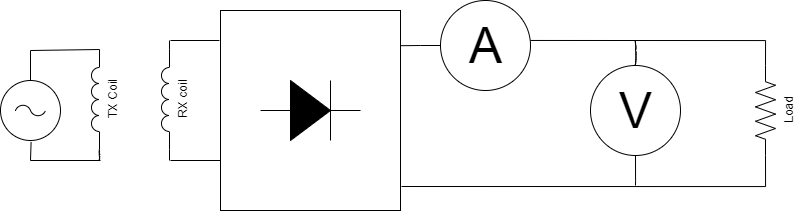
\includegraphics[width=0.8\linewidth]{RX_EFF_TEST}
\caption{Receiver RF-DC Converter Efficiency Test Setup}
\end{figure}

\subsection{Receiver Battery Charger Tests}

\indent
The bench power supply current should initially be llimited to 1A and the initial voltage should be set to 20V.  There are two diode voltage drops (1.4V) in the full wave rectifier bridge circuit.  18.6V on charger input is high enough for the proper operating voltage for the LTC4162-L battery charger.  The charger is functional without the battery pack and according to the datasheet, the voltage on the charger output will rise to the programmed constant-voltage value. By measuring this voltage it is possible to determine whether the charger regulates the proper voltage for a given programmed value.
\hfill 
\pagebreak
\hfill \\

\indent
A 18650 battery with two cells in series discharged to 3.2-3.8V per cell may be used for constant current and constant voltage charge testing.  The bench power supply should be connected followed by the battery and no change in MCU behavior should be noted. Constant current charging should begin.  The current limit of the bench power supply may be increased and the charging current should increase up to a maximum of 3.2A. The maximum charging current, charging voltage, cell count, and power supply current and voltage should be recorded and efficiency calculated.\\

\indent Then the power supply should be disconnected and reconnected and there should be no effect on the MCU power state. Charging should automatically resume when the power supply is reconnected. The battery should be allowed to charge until it enters constant voltage mode, which may be recognized by a slowly decreasing charge current that is much lower than the maximum current observed during constant current charging.  A 2 ohm load should be connected to the battery under charge for at least 30 seconds and removed without any effect on MCU operation.

\subsection{Receiver Firmware Tests}

\indent
The first recommendation in any trouble rise of troubleshooting of quality assurance is to check the mcu\_setup.c and mcu\_setup.h files.  Additionally, it is good to note that a unit test is a type of software test that only requires building a small portion of the codebase in order to test a set of specific modules.  Unit testing reduces the total amount of time dedicated into the development of any software.

%%% Currently at once every two seconds
\subsubsection*{The MCU Clock On LED} (MCU\_Clock\_on or D8 by the microcontroller) should be blinking at a rate of approximately twice every second \textbf{(This rate is subject to change)}.  If this is not occurring, the clock interrupt routine is not operating properly.  Investigate for over-polling at the UART RX Pins (P2.0 and P2.5) is occurring.  Alternatively, the TX Pins could be written out of turn (P2.1 and P2.6) which would thus initiate the UART Interrupts EUSCI\_A0\_VECTOR (located at P2.0 and P2.1) or EUSCI\_A1\_VECTOR (located at P2.5 and P2.6).  If this is not the case, the next step would be to troubleshoot the ADC (Analog to Digital Converter) Pins (P3.0, P3.1, P3.2, and P3.3).  If this issue where the ADC12\_B\_VECTOR interrupt contravenes the clock interrupt is detected, the error is likely caused by a breakdown in the hierarchy of interrupts.  In such a case, the code must be provided additional logic on how to handle specific interrupts in the scheduler’s run method.

\subsubsection*{The LCD Ticker Panel} should display some coherent statement or acronym.  If it does not, running of a “Hello World” unit test to the LCD is required for appropriate troubleshooting.  The unit test should utilize the identical function used in the production code.  If the unit test passes without errors, the error would reside in the accumulation of text that is meant to be passed into the LCD Ticker Panel.

\subsubsection*{The UART (RX/TX) CON} tests require unit tests. There are four unit tests to be done to test the non-Bluetooth UART ports (P2.5 and P2.6).  The first involves transmitting a ‘A’ character to the same PCB’s RX\_CON Pin (P2.5).  The next unit test would involve transmitting a string and acknowledgement TCP handshake.  These same unit tests are repeated with a secondary PCB.

\subsubsection*{The Bluetooth} validation tests will involve a unit test from the personal computer that connects to the receiver and sweeps through a set of pre-programmed unit tests that provide specific responses and sample data points.  The Bluetooth tests for the receiver should also include data requests pertaining to the voltage from the battery, the battery's current charge, and any data utilized in the battery charger.
\hfill \\
\pagebreak
\hfill
\section*{System Tests}
\subsection{Coil Test}
Coil impedance is measured using Vector Network Analyzer (VNA). The impedance measurement is obtained by setting the instrument to measure S-parameters (S11) at 13.56 MHz.  Before measurements, the instrument must be calibrated using calibration standards (short circuit, open circuit, and 50$\omega$ load).  The measured impedance is in complex form R+jX form.\\

\noindent
Specified inductance: 909.66nH\\

\noindent
The coil's inductance is determined using the formula below:
\begin{equation}
L = \frac{X_L}{\omega}
\end{equation}
\noindent
Where $\omega$ = 2$\pi$f\\

\noindent
The figure below shows the the equivalent circuit of how the transmitter / receiver coils were evaluated using a Vector Network Analyzer.
\hfill
\begin{figure}[h!]
\centering
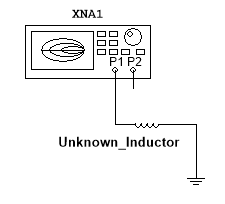
\includegraphics[width=0.5\linewidth]{RX_SUBSYSTEM_COIL_TERMINALS.PNG}
\caption{VNA Test Setup}
\end{figure}

\pagebreak

\noindent
Although VNA is not very precise for quality factor measurements it still can be used for estimation. The quality factor is determined by obtaining S21 parameter (forward voltage gain).\\

\noindent
Specified Q factor: 1119\\
 
 \noindent
The quality factor also can be determined by dividing reactance by the resistance the formula is shown below:
\begin{equation}
Q = \frac{X_L}{R}
\end{equation}

\subsection{System Level Firmware Tests}

\subsubsection*{The Bluetooth Localization Test} utilizes the “M” command on the RN4870 BLE chip with 3 prior locations to triangulate which direction is moving towards the transmitter.  This test begins with a computer provided unit test that accepts four distances, the first three that are used to triangulate the receiver in reference to the transmitter and a fourth that must be closer than all three triangulating distances to be considered passing.
\hfill 
\pagebreak

\subsection{Test Results Summary}

\subsubsection{Transmitter Evaluations} \hfill
\subsubsection*{DC Power Test} \hfill \\
\noindent
30V regulator no-load condition measured output voltage 30.04 V\\
5V regulator measured output voltage TP3 5.03V\\
3.3V regulator measured output voltage TP2 3.33V\\
 
\subsubsection*{Coil Driver Test} \hfill \\
Oscillator output voltage TP4 3.69V$_{pp}$\\
 
\noindent
Oscillator output Frequency (13.56 MHz) measured: 13.56MHz\\
Class E amplifier driver voltage jumper R32 (nominal 5Vpp) measured 5.80Vpp
\hfill
\begin{figure}[h!]
\centering
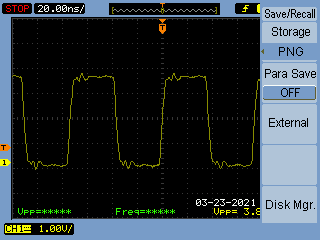
\includegraphics[width=0.8\linewidth]{osc_out}
\caption{Class E Amplifier Driver Output}
\end{figure}
\hfill \\
\pagebreak

\noindent
Q1 Dran nom. 117 V$_{pp}$ (30 V supply) Measured 102V$_{pp}$
\hfill
\begin{figure}[h!]
\centering
\includegraphics[width=0.65\linewidth]{Q1_measured}
\caption{Q1 Drain Voltage Waveform}
\end{figure}

\noindent
Transmitter coil voltage 117 V$_{pp}$ (30 V supply) Measured 204V$_{pp}$
\hfill
\begin{figure}[h!]
\centering
\includegraphics[width=0.65\linewidth]{t_coil_v_measured}
\caption{Q1 Drain Voltage Waveform}
\end{figure}
\hfill 
\pagebreak
\hfill \\
\noindent
Transmitter subsystem input current at 30V supply (120 mA nom. no laod) Measured 140 mA

\begin{table}[h!]
\centering
%Received Power (DC) vs Distance Test
\caption{Transmitted Power vs. Distance Test}
\begin{tabular}{ | c | c | c | }
\hline
 Distance [cm] & Measured Voltage [V$_{pp}$] & Received Power [W] \\
 \hline
5 & & \\
\hline
4 & & \\
\hline
3 & & \\
\hline
2 & & \\
\hline
1 & & \\
\hline
\end{tabular}
\end{table}

\subsubsection{Receiver Evaluations} \hfill \\
\subsubsection*{DC Power Test} \hfill \\
\noindent
5V regulator measured output voltage TP1 5.07V\\
3.3V regulator measured output voltage TP2 3.33V\\
18V regulator measured output voltage TP3 18.26V\\

\begin{table}[h!]
\centering
\caption{Received Power (DC) vs Distance Test}
\begin{tabular}{ | c | c | c |  c |}
\hline
Distance [cm] & Measured Voltage [V] & Measured Current [A] & Power Received [W] \\
\hline
5 & & & \\
\hline
4 & & & \\
\hline
3 & & & \\
\hline
2 & & & \\
\hline
1 & & & \\
\hline
\end{tabular}
\end{table}

\subsubsection*{Coil Design Verification Test}\hfill \\
\noindent
Specified inductance: 909.66nH\\ 
Measured impedance at 13.56MHz: 0.43 +j78.28$\Omega$\\
\hfill \\
\pagebreak
\hfill \\
\begin{figure}[h!]
\centering
\includegraphics[width=0.8\linewidth]{VNA_measured}
\caption{VNA TX/RX Coil Impedance Measurement}
\end{figure}
\hfill \\
\noindent 
Measured inductance using VNA (HP8753E) 0.917 $\mu$H\\
Measured inductance using LCR meter (HP4262A) 0.97$\mu$H\\
Q factor from VNA impedance measurement: 182
\hfill
\pagebreak
\section{Broader Impacts of the Project}

\indent
This product follows FDA, IEE, and government safety regulations. A few ethical issues faced by our design include high voltages across the coil, excessive heat generation within the receiver, and electromagnetic field interference. During simulation stages, high voltages were observed across the coil which increases the risk of electric shock hazard. In order to lower this risk, the coil insulation will adhere to a wider voltage range. Within the receiver, excessive heat generation along high current levels can cause damage to batteries. Therefore, lower charging currents will be used in order to prevent damage. Excessive heat also increases the cost of the project as fans would need to be added. Electromagnetic field interference caused by the transmitter coil can disrupt the charging circuit and cause battery failure. To prevent this issue, additional shielding will be implemented. \\

\indent
During testing stages, minor ethical issues were faced by the design. Within the receiver board, there was an inductor that was not suited for a frequency of 13.56 MHz board causing failure, and our rectifier circuits caused more loading than expected when tested with a signal generator. Also, the 48V to 30V buck stage microcontroller failed during testing for reasons that are yet to be further investigated by the team. When components get too hot, there’s not only a risk of it failing, but also of leaking its chemicals which can be dangerous to human skin and eyes. Therefore, the group will adhere to safety procedures such as wearing Personal Protective Equipment (PPE). Another risk observed here is electrical shock hazard due to the overloading in the circuit. To prevent this, the group will continuously measure the circuit for abnormal values while testing.\\

\indent
Our project’s goal is to provide users a low-cost medium-power wireless charger. There are no products like this one in the market for a few reasons: chargers do not supply more than 5W via inductive charging, an existing industrial unit with same purposes as our product is priced at about \$2000 USD, and available wireless chargers are limited for charging a single type of device only. With our product, users will be able to charge a standard battery type and integrate it in their own design or use it for stand-alone operations. Our product communicates electronic circuits, electromagnetic fields, digital systems, and microprocessors concepts to the audience. This product will not only be a low-cost wireless charger option, it will also provide customers with a charger for mobile devices of all shapes and sizes, no wiring exposure, apply greater range of tolerance for misalignment when charging, and provide a compact charging area. \\

\indent
Our product will be useful to robotics hobbyists and inventors who are developing new products that require wireless charging, serve to influence kids and teenagers interested in STEM, can be used for research and development, and capitalized in OEM market.

\begin{table}[h!]
\centering
\caption*{Ethical and Professional Considerations}
\begin{tabular} {| r | c | }
\hline
\parbox{0.3\linewidth}{\raggedleft Public Health} &   \parbox{0.65\linewidth}{\hfill \\
$\cdot$ Medical Equipment RF Exposure \\ $\cdot$ Electrical Shock \\ $\cdot$ Chemical Exposure}\\
\hline
\parbox{0.3\linewidth}{\raggedleft Safety and Wellness} &   \parbox{0.65\linewidth}{\hfill \\
$\cdot$ RF Bandwidth Jamming \\ $\cdot$ Electrical Shock \\ $\cdot$ Chemical Exposure}\\
\hline
\parbox{0.3\linewidth}{\raggedleft Global Factors} &   \parbox{0.65\linewidth}{\hfill \\
$\cdot$ International Governing Bodies \\ $\cdot$ Sourcing Restrictions \\ $\cdot$ Inter-Market Penetrability}\\
\hline
\parbox{0.3\linewidth}{\raggedleft Societal Factors} &   \parbox{0.65\linewidth}{\hfill \\
$\cdot$ Open-Source Capitalization\\ $\cdot$ STEM Educational Resources \\ $\cdot$ Professional Organizations \\ $\cdot$ Customer Privacy \& Security}\\
\hline
\parbox{0.3\linewidth}{\raggedleft Environmental Factors} &   \parbox{0.65\linewidth}{\hfill \\
$\cdot$ Chemical Pollution\\ $\cdot$ User Environmental Awareness\\ $\cdot$ Emergency Shut Off Cases}\\
\hline
\parbox{0.3\linewidth}{\raggedleft Economic Factors} &   \parbox{0.65\linewidth}{\hfill \\
$\cdot$ Open-Source Capitalization\\ $\cdot$ Specialty Clientele\\ $\cdot$ Rapid Agile-Deployment\\ $\cdot$ Light-Weight Production}\\
\hline
\end{tabular}
\end{table}
\hfill \\

\section{Conclusion}

\indent
This conclusion reflects the current state of our testing and troubleshooting process. We expect to continue testing our prototype and resolving issues in order to bring performance as close as possible to our initial specifications.\\

\indent
The 5V LCD contrast control circuit on both boards failed due to a design error: the digital potentiometer chosen was not capable of controlling a voltage greater than the 3.3V digital supply voltage. The 5V supplied to the potentiometer simply fed into the 3.3V supply through the protection diodes until the circuit was disabled.\\

\indent
The 48V to 30V buck stage control IC on the transmitter board self-destructed for as-yet unknown reasons. No obvious design errors were found. Further diagnosis was postponed pending testing of the remainder of the board using a bench power supply.\\
\hfill \\
\pagebreak
\hfill \\

\indent
Initial tests of the battery charging circuit were successful. A test battery of two fully charged 18650 cells was correctly detected and not charged further. After partial discharge the charger entered a constant-voltage charging mode and charged the battery at a slowly decreasing current of approximately 1A. The receiver board continued to operate on battery power when simulated wireless power was removed. Further testing of constant current charging, telemetry, and the SMbus smart battery interface is pending.\\

\indent
Initial testing of the wireless power transfer resulted in a period of successful inductive power transfer and a brief success in achieving a resonant link. A failure on the transmitter board was traced to an inductor that was not suitable for operation at 13.56 Mhz. The inductor and damaged components were replaced and testing continued. A resonant link was achieved between the transmitter and receiver, but an unexpected transient destroyed the transmitter amplifier transistor. A more robust replacement will be installed for further testing.\\

\indent
In summation, our testing revealed a few avoidable design errors which can be corrected or managed until a major revision is possible. The greatest challenge our testing has revealed is controlling the high voltages and unexpected transients that even a moderate-power resonant link creates. We hope that the use of more robust components will make it possible to continue testing and characterizing the real-world performance of our wireless power circuit. A further challenge is minimizing the losses from the high-frequency rectification stage. Our initial tests indicate that switching losses in the full wave bridge rectifier are significant. As suggested by our faculty advisor, it is possible that half-wave rectification will prove more efficient than a full-wave bridge.\\

\indent
With the benefit of foresight, we would have made a few minor and one major change in our design process. The wireless power transfer circuit is the most original component of our design and ideally would have been prototyped and tested much earlier in the design process. More minor changes would include accepting the more limited selection of 3.3V LCD’s and deleting the 5V rail and support circuitry. The 48V transmitter power supply and buck stage was chosen to minimize current and provide headroom for adjustments to the wireless transmitter voltage, but further testing may prove that a 30V supply with no further conversion is sufficient.

\pagebreak

\section{References}

\section*{Software References}

Block diagrams were rendered in Windows Visio Standard 2019.\\
Multisim circuits simulated in NI Multisim V.14.2 2019.\\
PCB Schematics rendered in Altium-365.\\
CAD Drawings rendered in NanoCAD.\\
%% Need it include TI-TINA simulation software.\\

	%%%%%%%%%%%%%%%%%%%%%%%%%%%%%%%%%%%%%%%%%%
	%														 %
	%														 %
	%				Special Note on Print Bibliiography w/ .bib file				 %
	%														 %
	%	   \printbibliography[keyword={a},keyword={b}] --> keyword a AND keyword b 	 %
	%			\defbibfilter{example}{keyword={a} or keyword={b}}	 		 %
	%		   \printbibliography[filter=example] --> keyword a OR keyword b 			 %
	%														 %
	%														 %
	%%%%%%%%%%%%%%%%%%%%%%%%%%%%%%%%%%%%%%%%%%

\printbibliography[keyword={regulation},title={Regulatory References}]

\defbibfilter{DesignReference}{keyword={documentation} or keyword={design}}
\printbibliography[filter=DesignReference,title={Design References}]

\printbibliography[keyword={catelog},title={Catelogs for Parts Investigated}]


%\pagebreak

%%%% 	Setting Configuration for Sections on Table of Contents and Pages 	%%%%%

\addappheadtotoc

\setcounter{section}{0}

% In Line
\titleformat{\section}{\normalfont\filcenter}{APPENDIX \Alph{section}:}{1em}{\MakeUppercase} 
\titleformat{\subsection}{\normalfont\itshape}{\arabic{subsection}.}{1em}{}

% Table of Contents
%\renewcommand{\thesection}{\Alph{section}}
\renewcommand{\thesubsection}{\thesection.\arabic{subsection}}

%\cftsetindents{section}{1em}{10em}

%%%% 	Sections on Table of Contents and Pages Configured 	%%%%%


\pagebreak

\begin{appendices}

\section{Codes, Standards, and Constraints}
\begin{table}[h!]
\centering
\caption{Relevant Codes and Standards}
\begin{tabular} {| r | c | }
\hline
\parbox{0.17\linewidth}{\centering Organization} &   \parbox{0.772\linewidth}{\centering Engineering Standards}\\
\hline
\parbox{0.17\linewidth}{\raggedleft IEEE} &   \parbox{0.772\linewidth}{\hfill \\
IEEE C95.1-2005\\
This standard defines exposure limits to the electromagnetic field \\
This standard is adopted in many safety standards. \\
IEEE 1625-2008 \\
Standard for rechargeable batteries for multicell mobile computing devices.\\
IEEE 802.15.1 Bluetooth standard \\
}\\
\hline
\parbox{0.17\linewidth}{\raggedleft Government} &   \parbox{0.772\linewidth}{\hfill \\
FCC Part 15, FCC part 18\\
RF Power levels and communication links are defined by FCC Part 15 and Part 18.\\
The RF transmitter power level limits in the US are much higher than in some other countries.\\
FDA: 21 CFR 1000.15 FCC: KDB 680106 D01   \\
Both standards define exposure limits to electromagnetic fields.\\
The limits will be satisfied if the transmitter power is limited to 5W.\\
Higher power levels are allowed if proper safety measures are implemented.\\
}\\
\hline
\parbox{0.17\linewidth}{\raggedleft International} &   \parbox{0.772\linewidth}{\hfill \\
EN 55011:2016\\
This standard defines limits for unwanted emissions in the RF spectrum above 30MHz. \\
The proposed WPT charger system must follow limitations for unwanted emissions.\\
}\\
\hline
\end{tabular}
\end{table}
\hfill
\pagebreak

\section{User's Manual and Instructions}

\begin{center}
$<$The User's Manual is not written currently$>$\\
\end{center}

\pagebreak

\section{Coursework Related Knowledge and Skills}

\begin{table}[h!]
\centering
\caption{Coursework Related Knowledge and Skills Table}
\begin{tabular}{ | l | l | }
\hline
\parbox{0.4\linewidth}{\centering
\textbf{Courses}
} &  \parbox{0.5\linewidth}{\centering
\textbf{Knowledge / Skills}
}\\
\hline
\parbox{0.4\linewidth}{\raggedleft
EENG 3106 - Circuit Analysis I Lab
} &   \parbox{0.5\linewidth}{\hfill \\
Laboratory Technique
}\\
\hline
\parbox{0.4\linewidth}{\raggedleft
EENG 3305 - Linear Circuits Analysis II
} &   \parbox{0.5\linewidth}{\hfill \\
Circuit Analysis (RLC Circuits)
}\\
\hline
\parbox{0.4\linewidth}{\raggedleft
EENG 4109 - Electronic Circuit Analysis II Lab
} &   \parbox{0.5\linewidth}{\hfill \\
Laboratory Technique
}\\
\hline
\parbox{0.4\linewidth}{\raggedleft
EENG 4309 - Electronic Circuit Analysis II
} &   \parbox{0.5\linewidth}{\hfill \\
Amplifier Design\\
Electronic circuit-analysis (amplifiers and rectifier circuits)
}\\
\hline
\parbox{0.4\linewidth}{\raggedleft
EENG 3303 - Electromagnetic Fields
} &   \parbox{0.5\linewidth}{\hfill \\
Electromagnetic Theory\\
Inductor parameters (inductance and resistance calculations based on shape and wire cross-section area and length.
}\\
\hline
\parbox{0.4\linewidth}{\raggedleft
EENG 3302 - Digital Systems
} &   \parbox{0.5\linewidth}{\hfill \\
Digital Troubleshooting
}\\
\hline
\parbox{0.4\linewidth}{\raggedleft
EENG 3307 - Microprocessors
} &   \parbox{0.5\linewidth}{\hfill \\
Microcontroller Programming
}\\
\hline
\parbox{0.4\linewidth}{\raggedleft
EENG 4350 - Advanced Microprocessors
} &   \parbox{0.5\linewidth}{\hfill \\
Microcontroller Programming
}\\
\hline
\end{tabular}
\end{table}
\hfill
\pagebreak

\section{Receiver PCB Schematics}
\hfill
\begin{figure}[h!]
\centering
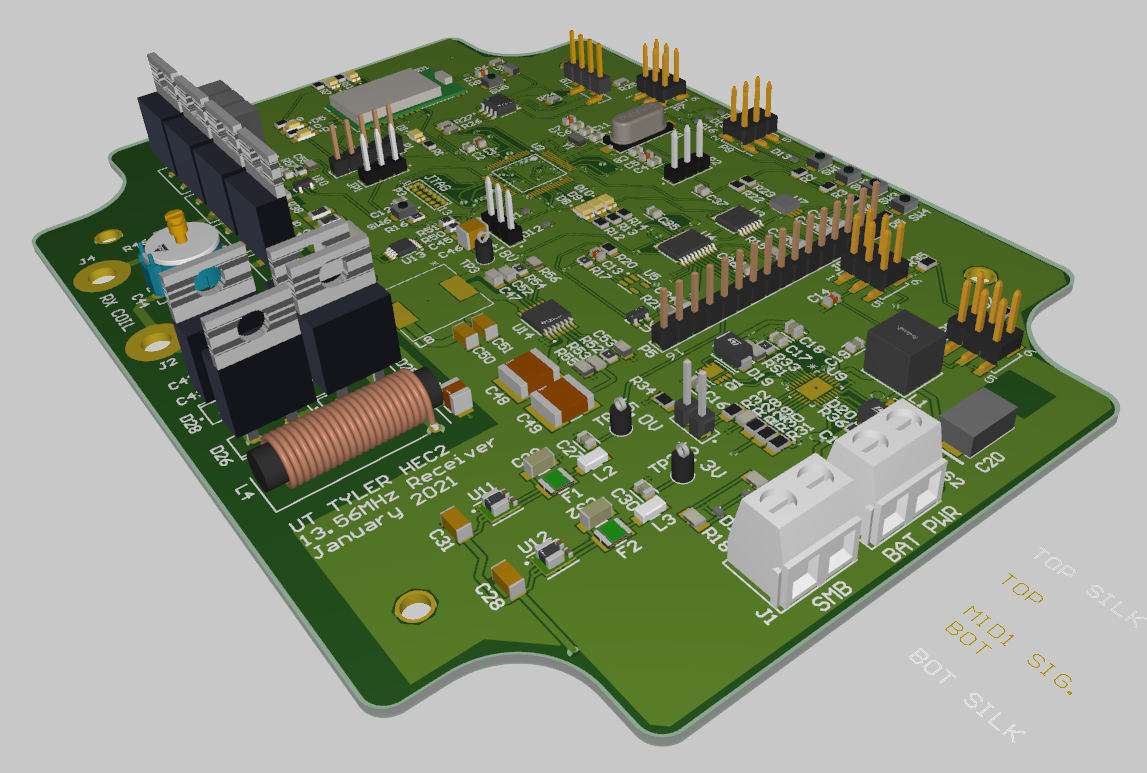
\includegraphics[angle=270, width=0.85\linewidth]{recv_pcb_img}
\caption{Isometric Image of Receiver PCB}
\end{figure}
\hfill
\pagebreak
\includepdf[pages=2,angle=90,width=0.95\linewidth,pagecommand=\subsection{Receiver Controller}]{./appendices/HEC2_Receiver.pdf}
\pagebreak
\includepdf[pages=3,angle=90,width=0.95\linewidth,pagecommand=\subsection{Receiver Battery Charger}]{./appendices/HEC2_Receiver.pdf}
\pagebreak
\includepdf[pages=4,angle=90,width=0.95\linewidth,pagecommand=\subsection{RF/DC Converter}]{./appendices/HEC2_Receiver.pdf}
\pagebreak
\includepdf[pages=5,angle=90,width=0.95\linewidth,pagecommand=\subsection{DC/DC Converter}]{./appendices/HEC2_Receiver.pdf}
\pagebreak
\includepdf[pages=6,angle=90,width=1.2\linewidth,pagecommand=\subsection{Top Copper Layer}]{./appendices/HEC2_Receiver.pdf}
\pagebreak
\includepdf[pages=7,angle=90,width=1.2\linewidth,pagecommand=\subsection{Top Silk Layer}]{./appendices/HEC2_Receiver.pdf}

\section{Transmitter PCB Schematics}
\hfill
\begin{figure}[h!]
\centering
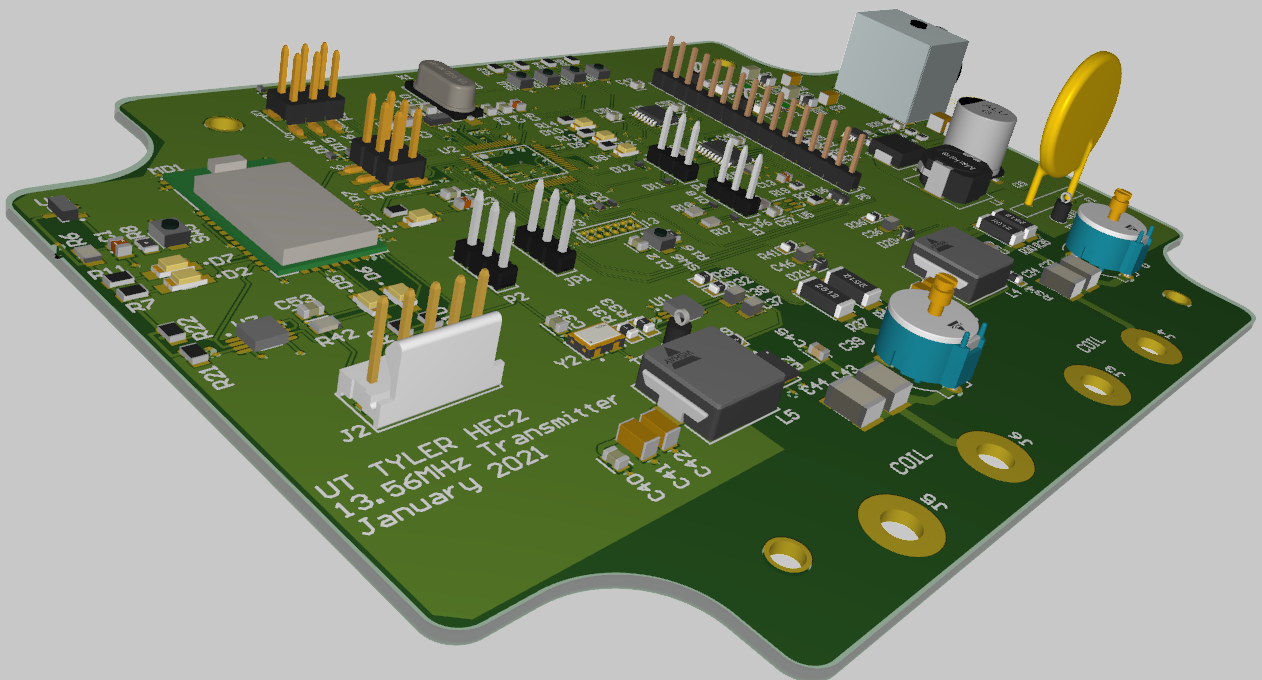
\includegraphics[angle=270, width=0.68\linewidth]{trans_pcb_img}
\caption{Isometric Image of Transmitter PCB}
\end{figure}
\hfill
\pagebreak
\includepdf[pages=2,angle=90,width=0.95\linewidth,pagecommand=\subsection{Transmitter Controller}]{./appendices/HEC2_Transmitter.pdf}
\pagebreak
\includepdf[pages=3,angle=90,width=0.95\linewidth,pagecommand=\subsection{DC/DC Converter}]{./appendices/HEC2_Transmitter.pdf}
\pagebreak
\includepdf[pages=4,angle=90,width=0.95\linewidth,pagecommand=\subsection{Coil Driver}]{./appendices/HEC2_Transmitter.pdf}
\pagebreak
\includepdf[pages=5,angle=90,trim={0 3in 7in 3in},clip,width=0.95\linewidth,pagecommand=\subsection{Top Copper Layer}]{./appendices/HEC2_Transmitter.pdf}
%\includepdf[pages=5,angle=90,width=1.2\linewidth,pagecommand=\subsection{Top Copper Layer}]{./appendices/HEC2_Transmitter.pdf}
\pagebreak
\includepdf[pages=6,angle=90,trim={0 3in 7in 3in},clip,width=0.95\linewidth,pagecommand=\subsection{Top Silk Layer}]{./appendices/HEC2_Transmitter.pdf}
%\includepdf[pages=6,angle=90,width=1.2\linewidth,pagecommand=\subsection{Top Silk Layer}]{./appendices/HEC2_Transmitter.pdf}
\pagebreak
\includepdf[pages=1,angle=90,width=0.95\linewidth,pagecommand=\section{Receiver BOM}]{./appendices/Receiver_BOM_RevA.pdf}
\pagebreak
\includepdf[pages={2-},angle=90,width=1.2\linewidth]{./appendices/Receiver_BOM_RevA.pdf}
\pagebreak
\includepdf[pages=1,angle=90,width=1.2\linewidth,pagecommand=\section{Transmitter BOM}]{./appendices/Transmitter_BOM_RevA.pdf}
\pagebreak
\includepdf[pages={2-},angle=90,width=1.2\linewidth]{./appendices/Transmitter_BOM_RevA.pdf}
\pagebreak
\includepdf[pages=1,angle=90,width=1.2\linewidth,pagecommand=\section{Wireless Power Transfer Module BOM}]{./appendices/Transmitter_WPT_SYSTEM_BOM_RevA.pdf}
\pagebreak
\section{Dimensional Coil Drawing}
\hfill
\begin{figure}[h!]
\centering
\includegraphics[angle=90,width=0.70\linewidth]{Coil_CAD}
\caption{Dimensional Coil Drawing}
\end{figure}
\hfill
\pagebreak
\section{GUI Wireframe Diagram}
\hfill
\begin{figure}[h!]
\centering
\includegraphics[angle=90,width=0.74\linewidth]{gui_wireframe}
\caption{GUI Wireframe Diagram}
\end{figure}
\hfill

\pagebreak
\section{Experimental Data Collection Sheets}

\subsection{Transmitter Subsystem Data}

\begin{table}[h!]
\centering
\caption*{Transmitter Subsystem Data}
\begin{tabular}{ | c | c | }
\hline
\textbf{Power Supply Verification} & \textbf{Pass or Fail} \\
\hline
\parbox{0.5\linewidth}{\raggedright \hfill \\[-0.25 em]
30V power supply voltage nominal 30V +/-2\% Measured (TP1) \hfill \\[0.1 em]
} &  \parbox{0.4\linewidth}{\raggedright \hfill \\ [0.7 em]
\underline{\hspace{0.625in}} V  \hspace{0.125 in}Pass \space / \space  Fail \hfill \\ [0.3 em]
} \\
\hline
\parbox{0.5\linewidth}{\raggedright \hfill \\[-0.25 em]
3.3V regulator (U11) test point TP2 nominal voltage 3.3V  tolerance +/- 1.5\% \hfill \\[0.1 em]
} &  \parbox{0.4\linewidth}{\raggedright \hfill \\ [0.7 em]
\underline{\hspace{0.625in}} V  \hspace{0.125 in}Pass \space / \space  Fail \hfill \\ [0.3 em]
} \\
\hline
\parbox{0.5\linewidth}{\raggedright \hfill \\[-0.25 em]
5V regulator (U11) test point TP3 nominal voltage 5V  tolerance +/- 1.5\% \hfill \\[0.1 em]
} &  \parbox{0.4\linewidth}{\raggedright \hfill \\ [0.7 em]
\underline{\hspace{0.625in}} V  \hspace{0.125 in}Pass \space / \space  Fail \hfill \\ [0.3 em]
} \\ 
\hline
\parbox{0.5\linewidth}{\raggedright \hfill \\[-0.25 em]
Coil driver Circuit Test \hfill \\[0.1 em]
} &  \parbox{0.4\linewidth}{\raggedright \hfill \\ [0.7 em]
\underline{\hspace{0.625in}} V  \hspace{0.125 in}Pass \space / \space  Fail \hfill \\ [0.3 em]
} \\ 
\hline
\parbox{0.5\linewidth}{\raggedright \hfill \\[-0.25 em]
Verify functionality of Transmitter Sub-circuits \hfill \\[0.1 em]
} &  \parbox{0.4\linewidth}{\raggedright \hfill \\ [0.7 em]
\underline{\hspace{0.625in}} V  \hspace{0.125 in}Pass \space / \space  Fail \hfill \\ [0.3 em]
} \\ 
\hline
\parbox{0.5\linewidth}{\raggedright \hfill \\[-0.25 em]
Verify Functionality of U11 \hfill \\[0.1 em]
} &  \parbox{0.4\linewidth}{\raggedright \hfill \\ [0.7 em]
\underline{\hspace{0.625in}} V  \hspace{0.125 in}Pass \space / \space  Fail \hfill \\ [0.3 em]
} \\ 
\hline
\parbox{0.5\linewidth}{\raggedright \hfill \\[-0.25 em]
Voltage test for drain of the GaN FET \hfill \\[0.1 em]
} &  \parbox{0.4\linewidth}{\raggedright \hfill \\ [0.7 em]
\underline{\hspace{0.625in}} V  \hspace{0.125 in}Pass \space / \space  Fail \hfill \\ [0.3 em]
} \\ 
\hline
\parbox{0.5\linewidth}{\raggedright \hfill \\[-0.25 em]
Test Peak to Peak Voltage across load \hfill \\[0.1 em]
} &  \parbox{0.4\linewidth}{\raggedright \hfill \\ [0.7 em]
\underline{\hspace{0.625in}} V  \hspace{0.125 in}Pass \space / \space  Fail \hfill \\ [0.3 em]
} \\ 
\hline
\parbox{0.5\linewidth}{\raggedright \hfill \\[-0.25 em]
Test Transmitter Power Output \hfill \\[0.1 em]
} &  \parbox{0.4\linewidth}{\raggedright \hfill \\ [0.7 em]
\underline{\hspace{0.625in}} V  \hspace{0.125 in}Pass \space / \space  Fail \hfill \\ [0.3 em]
} \\ 
\hline
\end{tabular}
\end{table}
\noindent
\textbf{This process is repeated for distances of 5 cm, 4 cm, 3 cm, 2 cm, and 1 cm.}

\subsection{Receiver Regulators Subsystem Data}

\begin{table}[h!]
\centering
\caption*{Receiver Regulators Subsystem Data}
\begin{tabular}{ | c | c | }
\hline
\textbf{Power Supply Verification} & \textbf{Pass or Fail} \\
\hline
\parbox{0.5\linewidth}{\raggedright \hfill \\[-0.25 em]
DC voltage across coil terminals (J2 \& J4)
 \hfill \\[0.1 em]} &  \parbox{0.4\linewidth}{\raggedright \hfill \\ [0.7 em]
\underline{\hspace{0.625in}} V  \hspace{0.125 in}Pass \space / \space  Fail \hfill \\ [0.3 em]
} \\
\hline
\parbox{0.5\linewidth}{\raggedright \hfill \\[-0.25 em]
5V regulator (U11) test point TP3 nominal voltage 5V  tolerance +/- 1.5\%
\hfill \\[0.1 em]} &  \parbox{0.4\linewidth}{\raggedright \hfill \\ [0.7 em]
\underline{\hspace{0.625in}} V  \hspace{0.125 in}Pass \space / \space  Fail \hfill \\ [0.3 em]
} \\
\hline
\parbox{0.5\linewidth}{\raggedright \hfill \\[-0.25 em]
3.3V regulator (U11) test point TP2 nominal voltage 3.3V  tolerance +/- 1.5\%
\hfill \\[0.1 em]} &  \parbox{0.4\linewidth}{\raggedright \hfill \\ [0.7 em]
\underline{\hspace{0.625in}} V  \hspace{0.125 in}Pass \space / \space  Fail \hfill \\ [0.3 em]
} \\ 
\hline
\parbox{0.5\linewidth}{\raggedright \hfill \\[-0.25 em]
Firmware Test Successful Load
\hfill \\[0.1 em]} &  \parbox{0.4\linewidth}{\raggedright \hfill \\ [0.7 em]
\underline{\hspace{0.625in}} V  \hspace{0.125 in}Pass \space / \space  Fail \hfill \\ [0.3 em]
} \\ 
\hline
\end{tabular}
\end{table}
\hfill \\
\pagebreak

\subsection{Receiver Rectifier Subsystem Data}

\begin{table}[h!]
\centering
\caption*{Receiver Rectifier Subsystem Data}
\begin{tabular}{ | c | c | }
\hline
\textbf{Efficiency Test Protocols} & \textbf{Parameters} \\
\hline
\parbox{0.5\linewidth}{\raggedright \hfill \\[-0.25 em]
The transmitter RF output
 \hfill \\[0.1 em]} & 
 30 W\\
\hline
\parbox{0.5\linewidth}{\raggedright \hfill \\[-0.25 em]
The receiver coil placement (parallel)
\hfill \\[0.1 em]} & 
5 cm\\
\hline
\parbox{0.5\linewidth}{\raggedright \hfill \\[-0.25 em]
Current measured
\hfill \\[0.1 em]} &  \parbox{0.4\linewidth}{\raggedright \hfill \\ [0.7 em] \underline{\hspace{0.625in}} 
A 
\hspace{0.125 in}Pass \space / \space  Fail \hfill \\ [0.3 em]} \\ 
\hline
\parbox{0.5\linewidth}{\raggedright \hfill \\[-0.25 em]
Load Voltage measured
\hfill \\[0.1 em]} &  \parbox{0.4\linewidth}{\raggedright \hfill \\ [0.7 em]\underline{\hspace{0.625in}} 
V  
\hspace{0.125 in}Pass \space / \space  Fail \hfill \\ [0.3 em]} \\ 
\hline
\parbox{0.5\linewidth}{\raggedright \hfill \\[-0.25 em]
Load Power
\hfill \\[0.1 em]} &  \parbox{0.4\linewidth}{\raggedright \hfill \\ [0.7 em]\underline{\hspace{0.625in}} 
W
\hspace{0.125 in}Pass \space / \space  Fail \hfill \\ [0.3 em]} \\ 
\hline
\parbox{0.5\linewidth}{\raggedright \hfill \\[-0.25 em]
Efficiency
\hfill \\[0.1 em]} &  \parbox{0.4\linewidth}{\raggedright \hfill \\ [0.7 em]\underline{\hspace{0.625in}} 
\%
\hspace{0.125 in}Pass \space / \space  Fail \hfill \\ [0.3 em]} \\ 
\hline
\end{tabular}
\end{table}
\noindent
\textbf{This process is repeated for distances of 5 cm, 4 cm, 3 cm, 2 cm, and 1 cm.}

\subsection{Charger Subsystem Data}

\begin{table}[h!]
\centering
\caption*{Charger Subsystem Data}
\begin{tabular}{ | c | c | }
\hline
\textbf{Test Protocols} & \textbf{Parameters} \\
\hline
\parbox{0.5\linewidth}{\raggedright \hfill \\[-0.25 em]
Set bench power supply current limit
 \hfill \\[0.1 em]} & 
 1 A \\
\hline
\parbox{0.5\linewidth}{\raggedright \hfill \\[-0.25 em]
Set initial voltage
\hfill \\[0.1 em]} & 
20 V\\
\hline
\parbox{0.5\linewidth}{\raggedright \hfill \\[-0.25 em]
Verify Charger Input Voltage
\hfill \\[0.1 em]} &  
18.6 V\\
\hline
\parbox{0.5\linewidth}{\raggedright \hfill \\[-0.25 em]
Voltage Charger Output
\hfill \\[0.1 em]} &  \parbox{0.4\linewidth}{\raggedright \hfill \\ [0.7 em] \underline{\hspace{0.625in}} 
V 
\hspace{0.125 in}Pass \space / \space  Fail \hfill \\ [0.3 em]} \\ 
\hline
\end{tabular}
\end{table}
\hfill \\
\pagebreak

\subsection{SMBus Subsystem Test  Data}

\begin{table}[h!]
\centering
\caption*{SMBus Subsystem Test Data}
\begin{tabular}{ | c | c | }
\hline
\textbf{Test Protocols} & \textbf{Parameters} \\
\hline
\parbox{0.5\linewidth}{\raggedright \hfill \\[-0.25 em]
Verify Interface Functionality
\hfill \\[0.1 em]} &  \parbox{0.4\linewidth}{\centering \hfill \\ [0.7 em] 
Pass \space / \space  Fail \hfill \\ [0.3 em]} \\ 
\hline
\parbox{0.5\linewidth}{\raggedright \hfill \\[-0.25 em]
Input Undervoltage Setting
\hfill \\[0.1 em]} &  \parbox{0.4\linewidth}{\raggedright \hfill \\ [0.7 em]\underline{\hspace{0.625in}} 
V  
\hspace{0.125 in}Pass \space / \space  Fail \hfill \\ [0.3 em]} \\ 
\hline
\parbox{0.5\linewidth}{\raggedright \hfill \\[-0.25 em]
Final Charge Voltage
\hfill \\[0.1 em]} &  \parbox{0.4\linewidth}{\raggedright \hfill \\ [0.7 em]\underline{\hspace{0.625in}} 
V
\hspace{0.125 in}Pass \space / \space  Fail \hfill \\ [0.3 em]} \\ 
\hline
\parbox{0.5\linewidth}{\raggedright \hfill \\[-0.25 em]
Target Charge Current
\hfill \\[0.1 em]} &  \parbox{0.4\linewidth}{\raggedright \hfill \\ [0.7 em]\underline{\hspace{0.625in}} 
A
\hspace{0.125 in}Pass \space / \space  Fail \hfill \\ [0.3 em]} \\ 
\hline
\parbox{0.5\linewidth}{\raggedright \hfill \\[-0.25 em]
Input Current Limit Target
\hfill \\[0.1 em]} &  \parbox{0.4\linewidth}{\raggedright \hfill \\ [0.7 em]\underline{\hspace{0.625in}} 
A
\hspace{0.125 in}Pass \space / \space  Fail \hfill \\ [0.3 em]} \\ 
\hline
\end{tabular}
\end{table}

\subsection{Coil Subsystem Test Data}
\begin{table}[h!]
\centering
\caption*{Coil Subsystem Test Data}
\begin{tabular}{ | c | c | }
\hline
\textbf{Test Protocols} & \textbf{Parameters} \\
\hline
\parbox{0.5\linewidth}{\raggedright \hfill \\[-0.25 em]
Calibration Test for Short Circuit
\hfill \\[0.1 em]} &  \parbox{0.4\linewidth}{\raggedright \hfill \\ [0.7 em] \underline{\hspace{0.625in}} 
$\mu$H
\hspace{0.125 in}Pass \space / \space  Fail \hfill \\ [0.3 em]} \\ 
\hline
\parbox{0.5\linewidth}{\raggedright \hfill \\[-0.25 em]
Calibration Test for Open Circuit
\hfill \\[0.1 em]} &  \parbox{0.4\linewidth}{\raggedright \hfill \\ [0.7 em]\underline{\hspace{0.625in}} 
$\mu$H
\hspace{0.125 in}Pass \space / \space  Fail \hfill \\ [0.3 em]} \\ 
\hline
\parbox{0.5\linewidth}{\raggedright \hfill \\[-0.25 em]
Calibration Test with 50$\Omega$ Resistive Load
\hfill \\[0.1 em]} &  \parbox{0.4\linewidth}{\raggedright \hfill \\ [0.7 em]\underline{\hspace{0.625in}} 
$\mu$H
\hspace{0.125 in}Pass \space / \space  Fail \hfill \\ [0.3 em]} \\ 
\hline
\parbox{0.5\linewidth}{\raggedright \hfill \\[-0.25 em]
Inductive Reactance
\hfill \\[0.1 em]} &  \parbox{0.4\linewidth}{\raggedright \hfill \\ [0.7 em]\underline{\hspace{0.625in}} 
j$\Omega$
\hspace{0.125 in}Pass \space / \space  Fail \hfill \\ [0.3 em]} \\ 
\hline
\parbox{0.5\linewidth}{\raggedright \hfill \\[-0.25 em]
Impedance
\hfill \\[0.1 em]} &  \parbox{0.4\linewidth}{\raggedright \hfill \\ [0.7 em]\underline{\hspace{0.625in}} 
$\Omega$
\hspace{0.125 in}Pass \space / \space  Fail \hfill \\ [0.3 em]} \\ 
\hline
\parbox{0.5\linewidth}{\raggedright \hfill \\[-0.25 em]
Quality Factor Estimation
\hfill \\[0.1 em]} &  \parbox{0.4\linewidth}{\raggedright \hfill \\ [0.7 em]\underline{\hspace{0.625in}} 
\hspace{0.125 in}Pass \space / \space  Fail \hfill \\ [0.3 em]} \\ 
\hline
\parbox{0.5\linewidth}{\raggedright \hfill \\[-0.25 em]
S$_{21}$ parameter (Forward Voltage Gain)
\hfill \\[0.1 em]} &  \parbox{0.4\linewidth}{\raggedright \hfill \\ [0.7 em]\underline{\hspace{0.625in}} 
\hspace{0.125 in}Pass \space / \space  Fail \hfill \\ [0.3 em]} \\ 
\hline
\end{tabular}
\end{table}
\hfill


\end{appendices}



%\pagebreak



	%%%%%%%%%%%%%%%%%%%%%%%%%%%%%%%%%%%%%%%%%%
	%														 %
	%														 %
	%		\pagenumbering{gobble}	"gobbles" or removes the pagination of the page  	 %
	%					and the following pages.						 %
	%														 %
	%		\pagenumbering{num_style}	sets the pagination of the page and 	  	 %
	%						the following pages						 %
	%														 %
	%						{num_style} List:						 %
	%														 %
	%				{roman} -> lowercase roman numerals           				 %
	%				{Roman} -> uppercase roman numerals           				 %
	%				{alph} -> lowercase alphabetical numerals           			 %
	%				{Alph} -> uppercase alphabetical numerals           			 %
	%				{arabic} -> standard decimal numerals (0-9)           			 %
	%														 %
	%			Altering \pagenumbering{} will restart the pagination at 1.			 %
	%			     See other tutorial for greater control of paginations.			 %
	%														 %
	%														 %
	%%%%%%%%%%%%%%%%%%%%%%%%%%%%%%%%%%%%%%%%%%




	%%%%%%%%%%%%%%%%%%%%%%%%%%%%%%%%%%%%%%%%%%
	%														 %
	%														 %
	%					Special Note on Quotation Marks					 %
	%														 %
	%			   Standard Quotation Mark (") --> right quotation mark			 %
	%			Double Reverse Accent Mark (``) --> left quotation mark	 		 %
	%			left quotation mark = \textquotedblleft vs \textquotedblright 		 %
	%														 %
	%														 %
	%%%%%%%%%%%%%%%%%%%%%%%%%%%%%%%%%%%%%%%%%%



	%%%%%%%%%%%%%%%%%%%%%%%%%%%%%%%%%%%%%%%%%%
	%														 %
	%														 %
	%					Special Note on Tables						 %
	%														 %
	%				   l = left, c = center, r = right alignment				 %
	%			   | in tabular sets borders between alignment sets		 		 %
	%	      \hline places a horizontal line across width of table above current the line  		 %
	%			   \\ (the endline command) begins next line of table.		 		 %
	%														 %
	%														 %
	%%%%%%%%%%%%%%%%%%%%%%%%%%%%%%%%%%%%%%%%%%


\end{document}




%%%%%%%%%%%%%%%%%%%%%%%%%%%%%%%%%%%%%%%%%%%%%%%%%%%%%%
%					 													  %
%					 													  %
%					  ALWAYS END THE DOCUMENT WITH								  %
%					 													  %
%							\end{document}									  %
%					 													  %
%					 													  %
%%%%%%%%%%%%%%%%%%%%%%%%%%%%%%%%%%%%%%%%%%%%%%%%%%%%%%